% Generated by Sphinx.
\def\sphinxdocclass{report}
\documentclass[letterpaper,10pt,english]{sphinxmanual}
\usepackage[utf8]{inputenc}
\DeclareUnicodeCharacter{00A0}{\nobreakspace}
\usepackage[T1]{fontenc}
\usepackage{babel}
\usepackage{times}
\usepackage[Bjarne]{fncychap}
\usepackage{longtable}
\usepackage{sphinx}
\usepackage{multirow}


\title{Cyclus Documentation}
\date{October 02, 2012}
\release{0.1}
\author{Robert Carlsen}
\newcommand{\sphinxlogo}{}
\renewcommand{\releasename}{Release}
\makeindex

\makeatletter
\def\PYG@reset{\let\PYG@it=\relax \let\PYG@bf=\relax%
    \let\PYG@ul=\relax \let\PYG@tc=\relax%
    \let\PYG@bc=\relax \let\PYG@ff=\relax}
\def\PYG@tok#1{\csname PYG@tok@#1\endcsname}
\def\PYG@toks#1+{\ifx\relax#1\empty\else%
    \PYG@tok{#1}\expandafter\PYG@toks\fi}
\def\PYG@do#1{\PYG@bc{\PYG@tc{\PYG@ul{%
    \PYG@it{\PYG@bf{\PYG@ff{#1}}}}}}}
\def\PYG#1#2{\PYG@reset\PYG@toks#1+\relax+\PYG@do{#2}}

\def\PYG@tok@gd{\def\PYG@tc##1{\textcolor[rgb]{0.63,0.00,0.00}{##1}}}
\def\PYG@tok@gu{\let\PYG@bf=\textbf\def\PYG@tc##1{\textcolor[rgb]{0.50,0.00,0.50}{##1}}}
\def\PYG@tok@gt{\def\PYG@tc##1{\textcolor[rgb]{0.00,0.25,0.82}{##1}}}
\def\PYG@tok@gs{\let\PYG@bf=\textbf}
\def\PYG@tok@gr{\def\PYG@tc##1{\textcolor[rgb]{1.00,0.00,0.00}{##1}}}
\def\PYG@tok@cm{\let\PYG@it=\textit\def\PYG@tc##1{\textcolor[rgb]{0.25,0.50,0.56}{##1}}}
\def\PYG@tok@vg{\def\PYG@tc##1{\textcolor[rgb]{0.73,0.38,0.84}{##1}}}
\def\PYG@tok@m{\def\PYG@tc##1{\textcolor[rgb]{0.13,0.50,0.31}{##1}}}
\def\PYG@tok@mh{\def\PYG@tc##1{\textcolor[rgb]{0.13,0.50,0.31}{##1}}}
\def\PYG@tok@cs{\def\PYG@tc##1{\textcolor[rgb]{0.25,0.50,0.56}{##1}}\def\PYG@bc##1{\colorbox[rgb]{1.00,0.94,0.94}{##1}}}
\def\PYG@tok@ge{\let\PYG@it=\textit}
\def\PYG@tok@vc{\def\PYG@tc##1{\textcolor[rgb]{0.73,0.38,0.84}{##1}}}
\def\PYG@tok@il{\def\PYG@tc##1{\textcolor[rgb]{0.13,0.50,0.31}{##1}}}
\def\PYG@tok@go{\def\PYG@tc##1{\textcolor[rgb]{0.19,0.19,0.19}{##1}}}
\def\PYG@tok@cp{\def\PYG@tc##1{\textcolor[rgb]{0.00,0.44,0.13}{##1}}}
\def\PYG@tok@gi{\def\PYG@tc##1{\textcolor[rgb]{0.00,0.63,0.00}{##1}}}
\def\PYG@tok@gh{\let\PYG@bf=\textbf\def\PYG@tc##1{\textcolor[rgb]{0.00,0.00,0.50}{##1}}}
\def\PYG@tok@ni{\let\PYG@bf=\textbf\def\PYG@tc##1{\textcolor[rgb]{0.84,0.33,0.22}{##1}}}
\def\PYG@tok@nl{\let\PYG@bf=\textbf\def\PYG@tc##1{\textcolor[rgb]{0.00,0.13,0.44}{##1}}}
\def\PYG@tok@nn{\let\PYG@bf=\textbf\def\PYG@tc##1{\textcolor[rgb]{0.05,0.52,0.71}{##1}}}
\def\PYG@tok@no{\def\PYG@tc##1{\textcolor[rgb]{0.38,0.68,0.84}{##1}}}
\def\PYG@tok@na{\def\PYG@tc##1{\textcolor[rgb]{0.25,0.44,0.63}{##1}}}
\def\PYG@tok@nb{\def\PYG@tc##1{\textcolor[rgb]{0.00,0.44,0.13}{##1}}}
\def\PYG@tok@nc{\let\PYG@bf=\textbf\def\PYG@tc##1{\textcolor[rgb]{0.05,0.52,0.71}{##1}}}
\def\PYG@tok@nd{\let\PYG@bf=\textbf\def\PYG@tc##1{\textcolor[rgb]{0.33,0.33,0.33}{##1}}}
\def\PYG@tok@ne{\def\PYG@tc##1{\textcolor[rgb]{0.00,0.44,0.13}{##1}}}
\def\PYG@tok@nf{\def\PYG@tc##1{\textcolor[rgb]{0.02,0.16,0.49}{##1}}}
\def\PYG@tok@si{\let\PYG@it=\textit\def\PYG@tc##1{\textcolor[rgb]{0.44,0.63,0.82}{##1}}}
\def\PYG@tok@s2{\def\PYG@tc##1{\textcolor[rgb]{0.25,0.44,0.63}{##1}}}
\def\PYG@tok@vi{\def\PYG@tc##1{\textcolor[rgb]{0.73,0.38,0.84}{##1}}}
\def\PYG@tok@nt{\let\PYG@bf=\textbf\def\PYG@tc##1{\textcolor[rgb]{0.02,0.16,0.45}{##1}}}
\def\PYG@tok@nv{\def\PYG@tc##1{\textcolor[rgb]{0.73,0.38,0.84}{##1}}}
\def\PYG@tok@s1{\def\PYG@tc##1{\textcolor[rgb]{0.25,0.44,0.63}{##1}}}
\def\PYG@tok@gp{\let\PYG@bf=\textbf\def\PYG@tc##1{\textcolor[rgb]{0.78,0.36,0.04}{##1}}}
\def\PYG@tok@sh{\def\PYG@tc##1{\textcolor[rgb]{0.25,0.44,0.63}{##1}}}
\def\PYG@tok@ow{\let\PYG@bf=\textbf\def\PYG@tc##1{\textcolor[rgb]{0.00,0.44,0.13}{##1}}}
\def\PYG@tok@sx{\def\PYG@tc##1{\textcolor[rgb]{0.78,0.36,0.04}{##1}}}
\def\PYG@tok@bp{\def\PYG@tc##1{\textcolor[rgb]{0.00,0.44,0.13}{##1}}}
\def\PYG@tok@c1{\let\PYG@it=\textit\def\PYG@tc##1{\textcolor[rgb]{0.25,0.50,0.56}{##1}}}
\def\PYG@tok@kc{\let\PYG@bf=\textbf\def\PYG@tc##1{\textcolor[rgb]{0.00,0.44,0.13}{##1}}}
\def\PYG@tok@c{\let\PYG@it=\textit\def\PYG@tc##1{\textcolor[rgb]{0.25,0.50,0.56}{##1}}}
\def\PYG@tok@mf{\def\PYG@tc##1{\textcolor[rgb]{0.13,0.50,0.31}{##1}}}
\def\PYG@tok@err{\def\PYG@bc##1{\fcolorbox[rgb]{1.00,0.00,0.00}{1,1,1}{##1}}}
\def\PYG@tok@kd{\let\PYG@bf=\textbf\def\PYG@tc##1{\textcolor[rgb]{0.00,0.44,0.13}{##1}}}
\def\PYG@tok@ss{\def\PYG@tc##1{\textcolor[rgb]{0.32,0.47,0.09}{##1}}}
\def\PYG@tok@sr{\def\PYG@tc##1{\textcolor[rgb]{0.14,0.33,0.53}{##1}}}
\def\PYG@tok@mo{\def\PYG@tc##1{\textcolor[rgb]{0.13,0.50,0.31}{##1}}}
\def\PYG@tok@mi{\def\PYG@tc##1{\textcolor[rgb]{0.13,0.50,0.31}{##1}}}
\def\PYG@tok@kn{\let\PYG@bf=\textbf\def\PYG@tc##1{\textcolor[rgb]{0.00,0.44,0.13}{##1}}}
\def\PYG@tok@o{\def\PYG@tc##1{\textcolor[rgb]{0.40,0.40,0.40}{##1}}}
\def\PYG@tok@kr{\let\PYG@bf=\textbf\def\PYG@tc##1{\textcolor[rgb]{0.00,0.44,0.13}{##1}}}
\def\PYG@tok@s{\def\PYG@tc##1{\textcolor[rgb]{0.25,0.44,0.63}{##1}}}
\def\PYG@tok@kp{\def\PYG@tc##1{\textcolor[rgb]{0.00,0.44,0.13}{##1}}}
\def\PYG@tok@w{\def\PYG@tc##1{\textcolor[rgb]{0.73,0.73,0.73}{##1}}}
\def\PYG@tok@kt{\def\PYG@tc##1{\textcolor[rgb]{0.56,0.13,0.00}{##1}}}
\def\PYG@tok@sc{\def\PYG@tc##1{\textcolor[rgb]{0.25,0.44,0.63}{##1}}}
\def\PYG@tok@sb{\def\PYG@tc##1{\textcolor[rgb]{0.25,0.44,0.63}{##1}}}
\def\PYG@tok@k{\let\PYG@bf=\textbf\def\PYG@tc##1{\textcolor[rgb]{0.00,0.44,0.13}{##1}}}
\def\PYG@tok@se{\let\PYG@bf=\textbf\def\PYG@tc##1{\textcolor[rgb]{0.25,0.44,0.63}{##1}}}
\def\PYG@tok@sd{\let\PYG@it=\textit\def\PYG@tc##1{\textcolor[rgb]{0.25,0.44,0.63}{##1}}}

\def\PYGZbs{\char`\\}
\def\PYGZus{\char`\_}
\def\PYGZob{\char`\{}
\def\PYGZcb{\char`\}}
\def\PYGZca{\char`\^}
\def\PYGZsh{\char`\#}
\def\PYGZpc{\char`\%}
\def\PYGZdl{\char`\$}
\def\PYGZti{\char`\~}
% for compatibility with earlier versions
\def\PYGZat{@}
\def\PYGZlb{[}
\def\PYGZrb{]}
\makeatother

\begin{document}

\maketitle
\tableofcontents
\phantomsection\label{index::doc}


\emph{Cyclus} is a next-generation nuclear {\hyperref[basics/fcs_background::doc]{\emph{fuel cycle simulator}}} environment, providing flexibility to users
and developers through an agent-based approach.

A principal goal of \emph{Cyclus} is to present a
low barrier to adoption by new users and developers in order to
encourage them to join a vibrant community in an {\hyperref[basics/ecosystem::doc]{\emph{expanding ecosystem}}}.

Most Cyclus core code development at this time will be led by Paul Wilson,
Katy Huff, Matthew Gidden, and Robert Carlsen, the CNERG fuel cycle group.

Interested developers are welcome and encouraged to contribute but may
experience code instability in the early experimental stages of
the project. For inspiration and a notion of current research directions,
please consult our {\hyperref[basics/roadmap::doc]{\emph{development roadmap}}}.


\chapter{Important Features}
\label{index:important-features}\label{index:cyclus}\begin{itemize}
\item {} \begin{description}
\item[{Modeling Paradigm}] \leavevmode\begin{itemize}
\item {} 
discrete facilities with discrete material transactions

\item {} 
flexible design of new fuel cycles

\end{itemize}

\end{description}

\item {} \begin{description}
\item[{Software Development Principles}] \leavevmode\begin{itemize}
\item {} 
low barrier/rapid payback to adoption

\item {} 
minimal inherent technology assumptions

\item {} 
commonly used/available free software infrastructure

\end{itemize}

\end{description}

\item {} \begin{description}
\item[{User Interaction}] \leavevmode\begin{itemize}
\item {} 
common physics infrastructure

\item {} \begin{description}
\item[{different user interface layer for different user audiences, with varying levels of both input control and output exploration}] \leavevmode\begin{itemize}
\item {} 
varying levels of input control

\item {} 
varying levels of output exploration

\end{itemize}

\end{description}

\end{itemize}

\end{description}

\end{itemize}

The \emph{Cyclus} modeling paradigm will let users reconfigure the basic
building blocks of a simulation without changing the software. The
foundation of a simulation will be a commodity broker that collects
offers and requests from a set of facilities and matches them
according to some algorithm. The user will be able to select which
type of algorithm is used for each broker and for each facility by
selecting an appropriate plug-in module for each and configuring it
with a particular set of parameters defined by that module. Changing
the parameters of a module will change the performance with a fixed
algorithm defining the behavior, while selecting a different module
will completely change its behavior.


\chapter{Learn More}
\label{index:learn-more}
The \emph{Cyclus} project repository is located at
\href{http://github.com/cyclus/cyclus}{http://github.com/cyclus/cyclus}.

Although you do not have to register with github to
download and edit the code, if you desire your work to be integrated into the
cyclus mainline of development \emph{you must fork the cyclus core repository into
your own github account and submit `Pull Requests'}.


\section{Cyclus Fundamentals}
\label{basics/main::doc}\label{basics/main:cyclus-fundamentals}

\subsection{Introduction to the \emph{Cyclus} Fuel Cycle Simulator}
\label{basics/introduction:introduction-to-the-cyclus-fuel-cycle-simulator}\label{basics/introduction::doc}
The Computational Nuclear Engineering Research Group (CNERG) of the University
of  Wisconsin-Madison (UW) has been developing a next generation nuclear fuel
cycle simulation platform called \emph{Cyclus} whose genesis was driven by a variety
of gaps seen in previous fuel cycle simulation efforts.  Three major design and
development philosophies encompass the current fleet of fuel cycle simulators:
\begin{enumerate}
\item {} 
A desire for usability, thus developing a tool which begins with a simple
model in a visual development environment that aims to provide an intuitive
user interface (e.g. DYMOND, DANESS, VISION)

\item {} 
A desire for rapid prototyping, thus developing a tool which begins with
simple models in a scripting language that allows for quick answers to early
problems (e.g.  CAFCA, GENIUS v1)

\item {} 
A desire for detail/fidelity, thus developing a tool with an ad-hoc
combination of existing complex analysis tools (e.g. COSI)

\end{enumerate}

Experience has demonstrated that each of these philosophies can be hindered from
simulating some classes of interesting problems due to complexity limits.  In most cases this
complexity constrains first the usability of the tool followed by its
extendability due to increasingly convoluted dependencies. The final victim is
performance, as the ability to quickly solve simple problems is lost to the
desire to solve more complex ones.

In addition to these technical challenges, there is also an institutional
challenge.  A combination of closed development platforms and closed
development processes has made it difficult for an individual researcher to
incorporate their ideas into a fuel cycle systems analysis.  The ability to
combine existing systems simulation tools with data about new facilities or
fuel cycle concepts is so challenging that many researchers either choose to
avoid systems analysis altogether or to write their own simplified tool
(usually in category 2 above).  These new, special purpose fuel cycle
simulation tools involve a duplication of effort and generally lack any robust
benchmarking.

Each of these approaches lacks a design basis in computational science and
software development that can deliver the stated desired attributes of the
final software product:
\begin{itemize}
\item {} 
usability -- accommodating a wide range of user sophistication

\item {} 
performance -- solving simple problems in interactive time scales

\item {} 
fidelity -- accommodating many levels of detail/fidelity, commensurate with a range of user sophistication

\end{itemize}

A complete nuclear fuel cycle simulator requires modeling efforts in a wide
variety of physical and social science domains.  This places a premium on a
software development process that will facilitate fluid collaboration among a
large group of geographically dispersed developers.  With this constraint in
mind, a number of software development practices can be identified as highly
valuable for this effort:
\begin{itemize}
\item {} 
openness -- the process should have low institutional \& technical obstacles to collaboration

\item {} 
modularity -- a particular approach to modularity should be pursued to allow the core infrastructure to be independent of proprietary and/or sensitive data and/or models

\item {} 
extensibility -- attention to both robustness and flexibility allows for myriad potential developer extensions

\end{itemize}


\subsubsection{Mission}
\label{basics/introduction:mission}
\emph{Cyclus}  will be a nuclear fuel cycle systems analysis software platform that
encourages collaboration among a diverse set of researchers. Emphasis will be
placed on both ease of collaboration through modularity as well as ubiquity in
order to analyze a significant number of possible future fuel cycle scenarios
succinctly and consistently.


\subsubsection{Vision}
\label{basics/introduction:vision}
In order to accomplish this mission, the \emph{Cyclus} team has developed a vision
for the development of a next generation fuel cycle simulator that includes
elements of software architecture, software development process and
fundamental design paradigms.


\subsubsection{Current Status}
\label{basics/introduction:current-status}
\emph{Cyclus} is being developed in an open environment.  For the current status of \emph{Cyclus}, visit \href{http://cyclus.github.com}{http://cyclus.github.com}.


\paragraph{Software Process \& Architecture}
\label{basics/introduction:software-process-architecture}
As indicated above, the software architecture and accompanying development
process are critical to a simultaneously robust and flexible analysis platform.


\subparagraph{Open Source Development Process}
\label{basics/introduction:open-source-development-process}
The \emph{Cyclus} development framework employs a modern, open source philosophy
that ensures transparency, attracts contributions from a varied community of
collaborators, and guarantees institution-independent access to all potential
users. In this development path, a public source code repository provides
unhindered access to the \href{http://github.com/cyclus/cyclys}{fundamental simulation framework} and
\href{http://github.com/cyclus/cycamore}{basic fuel cycle process models} volunteered by developers.
Granting unfettered access only to
the \emph{Cyclus} engine allows for compartmentalization of the code and its input
data. Thus, secure and proprietary model developers can be similarly encouraged
to utilize the \emph{Cyclus} framework. This modern development model passively
distributes specialized content to interested research groups, and facilitates
parallel model development efforts by institutions with complimentary goals.
The transparency inherent in this type of open source development path also
facilitates code review by exposing available content to verification and
validation by collaborators with diverse areas of specialization and levels of
expertise.

Another aspect of this development process is a preference for open source
third party libraries where additional functionality is necessary and available
from such libraries.  This includes basic infrastructure such as file
input/output, as well as model-specific capabilities like integer programming
for network flow optimization.


\subparagraph{Dynamically-loadable Modules}
\label{basics/introduction:dynamically-loadable-modules}
Dynamically-loadable modules are the primary mechanism for extending \emph{Cyclus}
with new underlying models.  The primary benefit of this approach is
encapsulation: the trunk of the code is completely independent of the
individual models and all customization and extension is implemented only in
the loadable module.  A secondary benefit of this encapsulation is the ability
for contributors to choose different distribution and licensing strategies for
their contributions.  Finally, this strategy allows an individual developers
to explore different levels of complexity within their modules, including
wrapping other simulation tools as loadable modules for \emph{Cyclus}.


\subparagraph{Use Cases \& Visualization}
\label{basics/introduction:use-cases-visualization}
Because of the wide array of use cases for \emph{Cyclus}, flexibility in the user
interface is important to provide different kinds of users with different
experiences.  This is true for input generation as well as output
visualization.  A variety of graphical user interface modes have been designed
and will be implemented in parallel with the development of underlying modules.
The graphical interface should be extensible by loadable modules in the same
way as the core code to provide developers the same flexibility in managing
their input as they have in implementing their models.  Output visualization is
also important - the discrete facility/discrete material paradigm generates a
large volume of small data that needs to be aggregated in various ways to
provide context to a variety of users.


\paragraph{Modeling Paradigm}
\label{basics/introduction:modeling-paradigm}
The modeling paradigm adopted by \emph{Cyclus} includes a number of deeply embedded
fundamental concepts.  These basic design choices comprise the bedrock on which
most future design choices are made. The \emph{Cyclus} team recognizes the
accompanying inflexibility to the code and therefore does not anticipate that
these attributes will change.


\subparagraph{Discrete Facility \& Discrete Material Objects}
\label{basics/introduction:discrete-facility-discrete-material-objects}
The modeling infrastructure is designed such that every facility in a global
nuclear fuel cycle is treated individually.  While modeling options will exist
to allow collective action, this will be as a special case of the individual
facility basis.  Each facility will have two fundamental tasks: to transact
nuclear material with other facilities and to transform that nuclear material
from an input form to an output form.  These materials will be modeled as
discrete objects that exist for a finite time and whose composition and
transaction history is logged throughout the simulation.


\subparagraph{Market-based Material Transactions}
\label{basics/introduction:market-based-material-transactions}
The transaction of nuclear materials will take place in ``markets'' that act as
brokers to match a set of requests for material with a set of offers for that
material.  A variety of market models (see Vision: Software Architecture) will
be available to perform this broker role, but each market will act
independently of other markets.  Markets will used to model a variety of
decision making behaviors, not restricted to behaviors that simulate economic
activity.  Once the requests and offers have been matched, the facilities will
exchange material objects.


\subparagraph{Region-Institution-Facility Hierarchy}
\label{basics/introduction:region-institution-facility-hierarchy}
Every discrete facility in \emph{Cyclus} is owned by an institution that operates in
a geographic region.  An institution can be used to represent any entity that
may own and operate a facility such as a private corporation, a government
agency, or a non-governmental agency, among others.  A region can be used to
represent any geographic area, typically a politically relevant area such a
sub-national region (e.g. a U.S. State), a nation-state, or a super-national
region (e.g. the E.U.).  While some performance parameters of the facility may
depend on its institutional ownership or geographical location, the more
important use of this capability is to control the way in which a facility
engages in a market for trade of nuclear material based on by whom it is owned
and/or operated.


\subparagraph{Optimization and Sensitivity}
\label{basics/introduction:optimization-and-sensitivity}
While the market models that form the basis of material transactions represent
largely social constructs, there is an initial desire to minimize the direct
simulation of institutional decision making to seek optimal solutions.
Instead, the fundamental approach is to drive a single simulation with a large
multi-dimensional data set and then allow modern optimization technology to
seek globally optimal solutions based on global objective functions.  Since
institutional decision making tends to seek an optimal solution only for the
actor making that decision (local optimization), it may not lead to an outcome
that optimizes for the largest population of stakeholders.


\subsection{Fuel Cycle Simulators}
\label{basics/fcs_background:fuel-cycle-simulators}\label{basics/fcs_background::doc}
A nuclear fuel cycle simulator is a tool used to explore the impacts
of alternative nuclear fuel cycle choices, when considered as a full
system at a national or international level.  Fundamentally, a nuclear
fuel cycle simulator tracks the flow of materials through the nuclear
fuel cycle, accounting for processes such as enrichment,
transmutation, decay, and partition of isotopes.  From these material
flows, and information about the operation history of the associated
facilities, various metrics can be assessed for different nuclear fuel
cycle designs.  As such, economic, environmental and security metrics
can compared to support decision making on research, development and
deployment decisions for future fuel cycle facilities.

Fuel cycle simulators provide insights into important trends as
nuclear fuel cycles undergo technological transitions in an uncertain
socio-political environment.  As such, while it is important to
achieve an overall conservation of mass, there is typically a
trade-off between the accuracy of specific isotopic compositions and
the speed of calculation, given the inherent uncertainty of making
predictions in unknown socio-political futures.  Therefore, the
physics models used for each individual process in the fuel cycle are
generally low-order approximations based on higher order analysis.

Fuel cycle simulators are not designed to provide detailed simulations
of specific facilities; neither high-fidelity predictive simulation nor
virtual reality environments.


\subsubsection{History of Systems Analysis Tools}
\label{basics/fcs_background:history-of-systems-analysis-tools}
Historically, a variety of systems analysis tools have been developed
to study nuclear fuel cycles.  One category of tools has been derived
from detailed facility models, arranged in complex coupling schemes,
and validated with detailed measurements from real systems.  While
these tools offer a much more rigorous treatment of the physics, and
more confidence in specific results, they often require much more time
and expertise in the analyst to compute the results, and may offer
more precision in the physics than is warranted given the
socio-political uncertainty.  The other main category of tools is
typically derived from simplified systems models, with physics detail
and complexity added where necessary to improve the fidelity of
results, but preferring rapid computation to excessive precision.

Regardless of the development path, these systems analysis tools have
inherent assumptions, limitations in their underlying software
infrastructure, and constraints on the variety of nuclear fuel cycle
options that can be assessed.  Comparing the results from different
tools, often in order to generate confidence in them all, can be
challenging and frequently requires oversimplified problems that
preclude the use of the advanced features of any one tool.

That said, there are a number of tools that are currently used around
the world to support systems decision on nuclear fuel cycle options:
\begin{itemize}
\item {} 
VISION

\item {} 
DANESS

\item {} 
COSI

\item {} 
NUWASTE

\item {} 
CAFCA

\item {} 
NFCSim

\end{itemize}


\subsection{The \emph{Cyclus} Fuel Cycle Simulator Roadmap}
\label{basics/roadmap:the-cyclus-fuel-cycle-simulator-roadmap}\label{basics/roadmap::doc}
It is expected that external development contributing to the expansion
of the Fuel Cycle Simulator will grow in creative, unpredictable ways
in answer to the needs of the developers.  Moreover, particular use
cases and specific user interests are likely to drive the need for new
capability.

To help direct and inspire development in support of current and anticipated
use cases, the current \emph{Cyclus} development team has identified areas of
essential research areas as well as potential research ideas.


\subsubsection{Research Areas}
\label{basics/roadmap:research-areas}
A number of research areas related to \emph{Cyclus} have already been
identified, but others are certainly possible:
\begin{enumerate}
\item {} 
\emph{Cyclus} core infrastructure development

\item {} 
Market model development

\item {} 
Region model development and deployment scenarios

\item {} 
Reactor model development

\item {} 
Separations model development

\item {} 
Geologic repository \& waste form modeling

\item {} 
Graphical interfaces for input and visualization

\item {} 
Social science to determine important metrics and measures

\item {} 
Optimization and sensitivity infrastructure

\item {} 
Transportation

\item {} 
Non-proliferation analysis

\end{enumerate}


\subsubsection{Active Projects/Contributors}
\label{basics/roadmap:active-projects-contributors}\begin{itemize}
\item {} \begin{enumerate}
\setcounter{enumi}{20}
\item {} 
Wisconsin-Madison:

\end{enumerate}
\begin{itemize}
\item {} 
\href{http://github.com/cyclus/cyclus}{Cyclus} core infrastructure

\item {} 
\href{http://github.com/cyclus/cycamore}{Cycamore} base module package

\item {} 
\href{http://github.com/katyhuff/cyder}{Cyder} geologic repository modeling

\item {} 
\href{http://github.com/cyclus/cyclopts}{Cyclopts} optimization interface library

\end{itemize}

\item {} \begin{enumerate}
\setcounter{enumi}{20}
\item {} 
Texas at Austin

\end{enumerate}
\begin{itemize}
\item {} 
\href{http://github.com/cyclus/cycic}{Cycic} input control

\end{itemize}

\item {} \begin{enumerate}
\setcounter{enumi}{20}
\item {} 
Utah

\end{enumerate}
\begin{itemize}
\item {} 
\href{http://github.com/cyclus/cyclist}{Cyclist} output visualization

\end{itemize}

\end{itemize}


\subsubsection{Potential Research Ideas}
\label{basics/roadmap:potential-research-ideas}
In support of fuel cycle options analysis, modules representing specific
technologies and fuel cycles will contribute significantly to the usefulness of
the cyclus {\hyperref[basics/ecosystem::doc]{\emph{ecosystem}}}. Some specific concepts that have been identified as
potentially versatile models for anticipated fuel cycle modeling goals include a
number of creative Market, Region, Institution, and Facility Models.


\paragraph{Market Model Ideas}
\label{basics/roadmap:market-model-ideas}
Potential \textbf{Markets} that can be expected to be useful in some anticipated
use cases include contract markets, markets encapsulating fundamental commodity
market theories, markets employing political affinity to make resolution
decisions, markets supporting multipass material routing, and markets that
enable shadow fuel cycles for nuclear proliferation modeling.


\paragraph{Region Model Ideas}
\label{basics/roadmap:region-model-ideas}
Potential \textbf{Regions} include those supporting political affinity models of
international trade behavior, tax structures, creative growth patterns, political
instabilities capable of causing technology interruption, and international fuel
takeback agreeemnts.


\paragraph{Institution Model Ideas}
\label{basics/roadmap:institution-model-ideas}
Potentially compelling \textbf{Institutions} might support capacity dispatch logistics
similar to public utility commision behavior or define nuclear growth in the
presence of the growth of nonnuclear energy market share.


\paragraph{Facility Model Ideas}
\label{basics/roadmap:facility-model-ideas}
Myriad potential \textbf{Facilities} would support the broad {\hyperref[basics/ecosystem::doc]{\emph{ecosystem}}}
of models useful for fuel cycle options analysis. Facility models are the
technical building blocks of Cyclus simulations, and are expected to provide the
modular representation of essential nuclear, chemical, and industrial processes
in fuel cycles of all kinds. Potential fuel cycle technologies of import include
\begin{itemize}
\item {} 
advanced reactors

\item {} 
separations stoichiometry process modules

\item {} 
transportation modules

\item {} 
uranium resource models

\item {} 
nefarious shadow material diversion processes

\item {} 
random facility disruption

\end{itemize}


\paragraph{Full Simulation Scale Contributions}
\label{basics/roadmap:full-simulation-scale-contributions}
Additional simulation-level features envisioned to become useful in the near
term for optimization, economic, and strategic use cases include :
\begin{itemize}
\item {} 
external multi-variable optimization demonstration

\item {} 
objective functions for assessing overall simulation performance (e.g. economic)

\item {} 
investigation of impact of varying module fidelity

\item {} 
implementations of relevant simulation use cases, benchmarking cases, etc.

\end{itemize}


\subsection{The \emph{Cyclus} Community \& Ecosystem}
\label{basics/ecosystem::doc}\label{basics/ecosystem:the-cyclus-community-ecosystem}
An important goal of the \emph{Cyclus} effort is to attract a community of
developers contributing to a vibrant ecosystem of models for use by
users.  However, due to sensitivities regarding the distribution of
software for simulating nuclear systems, this ecosystem requires
careful considerations in its design and implementation.

Critical to the success of this community is the widespread
availability of the core infrastructure of the Cyclus simulation
environment.  Because this environment is formulated using a variety
of very generic concepts - not specific to nuclear energy systems -
this should mitigate concerns for the open source distribution of this
core infrastructure.

Moreover, this infrastructure is also designed to allow for the
addition of run-time modules, or plug-ins, that can be developed and
distributed under any possible licensing scheme.  These modules will
be distributed separately from the core infrastructure, and the
distribution responsibility will rest with the developer of each
module.  This system will insulate the core infrastructure from
accidental ``pollution'' by modules of a sensitive nature, and similarly
limit issues regarding the authorization for distribution to the
author's organization.  Ideally, most module developers will be
authorized for open distribution of their modules.

Finally, the community will be relied upon to provide review and
curation of available modules, establishing both quality assurance
practices and recommendations for best use cases for each contributed
module.

Below, a more detailed exposition of these characteristics is
provided.


\subsubsection{Open Source Core Infrastructure}
\label{basics/ecosystem:open-source-core-infrastructure}
The current portfolio of fuel cycle simulators has been characterized
by barriers to adoption by new users and developers including:
\begin{itemize}
\item {} 
policies of limited/restricted distribution,

\item {} 
reliance on propriety software development infrastructures, and

\item {} 
deeply embedded nuclear technology assumptions arising from
development path.

\end{itemize}

Since, one of the principle purposes of \emph{Cyclus} is to create a fuel
cycle simulator system with a low barrier to adoption, a policy of
open source distribution of this core infrastructure is critical to
its mission.  (\emph{Cyclus} is also committed to free and widely used
software development tools, such as GNU compilers, SQLite, Boost,
etc.)  The \emph{Cyclus} core is currently available via it's \href{http://github.com/cyclus/cyclus}{Git hub
repository}.  Interested users and
developers are invited to make their own copy of this repository,
review the list of open issues, and participate in the developers
mailing list. Like all open source projects, this distribution mode
permits a thorough code review by interested parties and the
possibility of contributions in order to identify/resolve defects or
request/provide feature enhancements.

The \emph{Cyclus} core infrastructure provides {\hyperref[devdoc/cyclus_env::doc]{\emph{a generic environment}}} for modeling flows of materials among a
collection of nuclear facilities.  This infrastructure could be used
for modeling many different supply chain systems, nuclear and
non-nuclear alike, although the introduction of features to this
infrastructure is prioritized to facilitate nuclear systems analysis.
In addition to addressing the barrier of deeply embedded nuclear
technology assumptions, one consequence of this approach is that the
core infrastructure has a very low risk of containing sensitive
information regarding the simulation of nuclear systems.  These
capabilities are added by acquiring and invoking plug-in modules
developed and distributed by the \emph{Cyclus} community.

The open source approach can also allow the project to leverage the
efforts a larger pool of developers and improve the quality of the
software product \footnote{
J.W. Paulson, \emph{et al}, ``An Empirical Study of Open-Source and Closed-Source Software Products'', \emph{IEEE Transactions on Software Engineering}, \textbf{30} (4), April 2004. \href{http://ieeexplore.ieee.org/stamp/stamp.jsp?arnumber=01274044}{http://ieeexplore.ieee.org/stamp/stamp.jsp?arnumber=01274044}
}.


\subsubsection{Decentralized Module Development \& Distribution}
\label{basics/ecosystem:decentralized-module-development-distribution}
When a user/developer wishes to contribute a new module to the
\emph{Cyclus} ecosystem, they will be responsible for all aspects of that
distribution.  The \emph{Cyclus} core development team will provide a
catalog of available modules (details are still under development),
but this catalog will point to external distribution sites that are
consistent with each contributors personal and/or institutional needs.
For example, developers who are permitted to follow an open source
approach with their own contributions can have their own Github
account and share their modules through the same mechanism as - but a
different location from - the \emph{Cyclus} core.  For some subset of open
source distribution mechanisms, the \emph{Cyclus} core will include tools
to make it easier for individual users to download and install
contributed modules or collections of modules.

Decentralizing the development and distribution of run-time plug-in
modules provides a number of benefits.  First, as is true for the core
infrastructure, this opens the door for a larger pool of developers to
contribute to the \emph{Cyclus} ecosystem, by providing modules that
represent their organizations specific technical interest.  If a
particular user/developer would like to understand the impact of their
own technology on the greater fuel cycle, they are free to develop a
module that simulates this technology and contribute it to the broader
community.

More importantly, this will contribute to the maintenance of a
``pristine'' core infrastructure, from the point of view of sensitive
information.  Since any software added to the source code repository
leaves behind permanent artifacts, even if removed at a later date,
inclusion of plug-in modules in a single common software repository
would pose the risk that the entire repository could be declared
sensitive at some future date.  Decentralized distribution mitigates
this risk.

Finally, this decentralized approach removes the burden of authorizing
distribution and reviewing contributions from a central authority.  A
centralized approach would require identifying a single organization
that would accept an ongoing burden of authorizing distribution,
assessing quality and assembling collections.  A decentralized
approach leaves those functions in the hands of the authors and
community as described in the following sections.


\paragraph{Distribution Authorization by Owner}
\label{basics/ecosystem:distribution-authorization-by-owner}
Between concerns for copyright and intellectual property, and the risk
that sensitive information could be inadvertently introduced into a
plug-in module, the burden of acquiring and confirming distribution
rights by a centralized organization could become prohibitive.  If,
instead, the \emph{Cyclus} ecosystem is captured in a catalog that refers
to a variety distribution sites as appropriate for each developer, the
effort for ensuring the rights for distribution are in the hands of
the developer and their organization.  The inclusion of a given module
in the catalog requires little oversight and the details of
distribution remain between the provider and consumer of each module.


\paragraph{Peer-review QA and Rating}
\label{basics/ecosystem:peer-review-qa-and-rating}
For most organizations, including a plug-in module in a centralized
software distribution would be regarded as a tacit approval of the
quality and utility of the module.  In most such cases, a substantial
burden of quality assurance and testing would be required by the
organization preforming this centralized distribution.  In the
decentralized approach of the \emph{Cyclus} ecosystem, mechanisms will be
provided for members of the community to provide peer-review of the
modules' quality and applicability to certain problems.

For modules that are distributed with an open source policy, other
users and developers will be able to perform a direct source code
review as well as testing the functionality of the module in a fuel
cycle analysis.  For other distribution policies, more limited review
will be possible.

In all cases, practices and policies will emerge from the community to
support standardization of this process.  For example, providing
adequate documentation and test suites will result in a better review
from members of the community and ultimately will become
pre-requisites to a positive peer review.


\paragraph{Curation and Collections}
\label{basics/ecosystem:curation-and-collections}
When the number of contributions is sufficiently large, there will be
benefit in developing collections of modules that are known to be
useful for certain types of simulations.  A decentralized approach
will allow individual members of the \emph{Cyclus} community to create such
collections, providing a curation function to help both new and
experienced users identify the modules that are likely to give them
the most benefit.


\subparagraph{Footnotes}
\label{basics/ecosystem:footnotes}

\subsection{Glossary of Cyclus Terms}
\label{basics/glossary:glossary-of-cyclus-terms}\label{basics/glossary::doc}\begin{description}
\end{description}
\begin{description}
\item[{\textbf{advanced users}}] \leavevmode
Similar to end users, but these users will desire more
sophisticated customization and level of detail.

\item[{\textbf{fuel cycle simulator}}] \leavevmode
A computational framework for modeling nuclear fuel cycles.

\item[{\textbf{commodity}}] \leavevmode
Something for which there is supply and/or demand that may be tradeable on a
market. Commodities usually have a one-to-one relationship with markets.

\item[{\textbf{plug-in}}] \leavevmode
See dynamically loadable module.

\item[{\textbf{closed development platform}}] \leavevmode
A code repository or server that is kept private during development to
secure proprietary or sensitive work.

\item[{\textbf{closed development process}}] \leavevmode
A software development workflow, usually on a closed platform, that is not
transparent to the public as authorization is required before development
access to the codebase is granted. This is used for secure proprietary or
sensitive work.

\item[{\textbf{cyclus core}}] \leavevmode
The repository at github.com/cyclus/cyclus contains only the simulation
engine. It links dynamically to modules contributed from other code
repositories. The library is called libcycluscore.

\item[{\textbf{developers}}] \leavevmode
Individuals from science, academia, government, or the general public
interested in contributing to the ecosystem of models available for use with
the simulator.

\item[{\textbf{dynamically loadable module}}] \leavevmode
A shared object or dynamic library representing a model class in Cyclus,
such as a Facility. It's functionality is linked at runtime to the
simulator.

\item[{\textbf{ecosystem}}] \leavevmode
A community of developers contributing to a vibrant ecosystem of models
for use by cyclus users.

\item[{\textbf{end users}}] \leavevmode
Members of the public who directly interface with the code, but
perhaps only through its graphical interface and have only a limited need for detail.

\item[{\textbf{extensibility}}] \leavevmode
An extensible code must be robust against changes and provide a flexibile
component interface for incorporating contributed modular code additions.

\item[{\textbf{maintainers}}] \leavevmode
These individuals are an advanced group of developers tasked with
moderating code contributions to the core of the cyclus code.

\item[{\textbf{model}}] \leavevmode
A conceptual representation used to represent something. In Cyclus, a
computational representation of some component (Market, Facility, etc.)
within the nuclear fuel cycle.

\item[{\textbf{modularity}}] \leavevmode
Best acheived by a framework with clear component interfaces, modularity is
an interchangeability of components such as data, classes, objects, or libraries
within a simulation. Modularity facilitates encapsulation and independence
of components that might be proprietary or sensitive.

\item[{\textbf{module}}] \leavevmode
A shared object or dynamic library representing a model class in Cyclus,
such as a Facility.

\item[{\textbf{nuclear fuel cycle}}] \leavevmode
The progression of nuclear fuel through the collection of facilities and
process stages from mining to disposal that are necessary to generate
nuclear power as well as to prepare, manage, recycle, and store nuclear fuel.

\item[{\textbf{open development platform}}] \leavevmode
A code repository or server that is publicly viewable and downloadable,
though not necessarily modifiable.

\item[{\textbf{open development process}}] \leavevmode
A software development workflow, usually on an open platform, that is
transparent to the public. Hallmarks include public bug reports, source code
access, and a  a member of the public to contribute code.

\item[{\textbf{openness}}] \leavevmode
A general notion that code, the development process, collaboration, and the
research it supports be unfettered by institutional, national, or other
boundaries, where possible.

\item[{\textbf{viewers}}] \leavevmode
Members of the public not directly interfacing with the code but to
whom the output may be made available for demonstration purposes.

\end{description}


\section{Cyclus User Guide}
\label{usrdoc/main::doc}\label{usrdoc/main:cyclus-user-guide}
Documentation to assist with the use of \emph{Cyclus} will be maintained on this
website and in the automated documentation generated via the \emph{Cyclus} source
code.

An instruction manual for {\hyperref[devdoc/get_and_build::doc]{\emph{Getting and Building Cyclus}}} is provided.
Questions having to do with this process may be directed to
\href{mailto:cyclus-dev@googlegroups.com}{cyclus-dev@googlegroups.com} .


\subsection{Creating and Running Simulations}
\label{usrdoc/creating_and_running_sims:creating-and-running-simulations}\label{usrdoc/creating_and_running_sims::doc}

\subsubsection{Cyclus Command Line Usage}
\label{usrdoc/creating_and_running_sims:cyclus-command-line-usage}
To run a simulation you must use the \emph{cyclus} command line utility:

\begin{Verbatim}[commandchars=\\\{\}]
./path/to/cyclus [options] [input-file]
\end{Verbatim}

\textbf{options}:
\begin{quote}
\begin{itemize}
\item {} 
\emph{-v{[}level{]}} where level is one of:
\begin{itemize}
\item {} 
\emph{LEV\_ERROR} (least verbose and the default if no verbosity is specified)

\item {} 
\emph{LEV\_WARN}

\item {} 
\emph{LEV\_INFO{[}1, 2, 3, 4, 5{]}}

\item {} 
\emph{LEV\_DEBUG{[}1, 2, 3, 4{]}}

\item {} 
\emph{LEV\_DEBUG5} (most verbose)

\end{itemize}

\end{itemize}

Note  that level can be specified as a number. Zero corresponds to
\emph{LEV\_ERROR}, and 11 corresponds to \emph{LEV\_DEBUG5}.
\end{quote}

\textbf{input file}:
\begin{quote}

The absolute or relative path (including the input file name itself) to the
input file to be run.
\end{quote}


\paragraph{Examples}
\label{usrdoc/creating_and_running_sims:examples}
\begin{Verbatim}[commandchars=\\\{\}]
./cyclus ./path/to/myinput.xml

./cyclus -v LEV\_DEBUG5 myinput.xml

./cyclus -v LEV\_INFO3 myinput.xml

./cyclus -v 4 myinput.xml
\end{Verbatim}


\section{Cyclus Developer Guide}
\label{devdoc/main:cyclus-developer-guide}\label{devdoc/main::doc}
Documentation to assist with the development of \emph{Cyclus} will be maintained
in a variety of forms.  If you haven't already, check out
{\hyperref[basics/main::doc]{\emph{Cyclus Fundamentals}}}

The \emph{Cyclus} project repository is located at
\href{http://github.com/cyclus/cyclus}{http://github.com/cyclus/cyclus}.

Although you do not have to register with github to
download and edit the code, if you desire your work to be integrated into the
cyclus mainline of development \emph{you must fork the cyclus core repository into
your own github account and submit `Pull Requests'}.


\subsection{Getting Started}
\label{devdoc/main:getting-started}
First things first - read {\hyperref[devdoc/get_and_build::doc]{\emph{Getting and Building Cyclus}}}.  After
successfully acquiring and building \emph{Cyclus}, you can begin developing:


\subsubsection{Getting and Building Cyclus}
\label{devdoc/get_and_build:getting-and-building-cyclus}\label{devdoc/get_and_build::doc}

\paragraph{The Cyclus Library Suite}
\label{devdoc/get_and_build:the-cyclus-library-suite}
\emph{Cyclus} is composed of a number of libraries:
\begin{itemize}
\item {} 
\href{https://github.com/cyclus/cyclus}{cyclus core} (basic functionality)

\item {} 
\href{https://github.com/cyclus/cycamore}{cycamore} (a module repository)

\item {} 
\href{https://github.com/cyclus/cyclopts}{cyclopts} (optimization)

\end{itemize}

This guide will describe how to install each library.


\paragraph{Dependencies}
\label{devdoc/get_and_build:dependencies}
Each of the above libraries has external dependencies, and some have
dependencies on others. The external libraries described below must
be installed in order to continue with the building and installing
process.


\subparagraph{Cyclopts}
\label{devdoc/get_and_build:id1}
Cyclopts is the optimization library of \emph{Cyclus}. It has the following
dependencies:
\begin{quote}

\begin{tabulary}{\linewidth}{|L|L|L|}
\hline
\textbf{
Package
} & \textbf{
Full Name
} & \textbf{
Minimum Version
}\\\hline

\emph{CMake}
 & 
cmake
 & 
2.8
\\\hline

\emph{boost}
 & 
libboost-all-dev
 & 
1.34.1
\\\hline

\emph{coin-Cbc}
 & 
coin-Cbc
 & 
2.7
\\\hline
\end{tabulary}

\end{quote}

The \href{https://projects.coin-or.org/Cbc}{coin} dependecy is the most
complicated of those above; full install instructions for coin-Cbc
are provided in the \href{https://github.com/cyclus/cyclopts}{cyclopts readme}.


\subparagraph{Core}
\label{devdoc/get_and_build:core}
The \emph{Cyclus} Core provides the basic agent-based modeling
functionality of the \emph{Cyclus} simulation engine. It has the
following dependencies:
\begin{quote}

\begin{tabulary}{\linewidth}{|L|L|L|}
\hline
\textbf{
Package
} & \textbf{
Full Name
} & \textbf{
Minimum Version
}\\\hline

\emph{CMake}
 & 
cmake
 & 
2.8
\\\hline

\emph{boost}
 & 
libboost-all-dev
 & 
1.34.1
\\\hline

\emph{xml2}
 & 
libxml2-dev
 & 
2
\\\hline

\emph{sqlite3}
 & 
libsqlite3-dev
 & 
3.7.10
\\\hline

\emph{coin-Cbc}
 & 
coin-Cbc
 & 
2.7
\\\hline

\emph{cyclopts}
 & 
cyclopts
 & 
present
\\\hline
\end{tabulary}

\end{quote}


\subparagraph{Cycamore}
\label{devdoc/get_and_build:id2}
Cycamore is a repository of all available modules which can be used
with the \emph{Cyclus} Core. It has the following dependencies:
\begin{quote}

\begin{tabulary}{\linewidth}{|L|L|L|}
\hline
\textbf{
Package
} & \textbf{
Full Name
} & \textbf{
Minimum Version
}\\\hline

\emph{CMake}
 & 
cmake
 & 
2.8
\\\hline

\emph{boost}
 & 
libboost-all-dev
 & 
1.34.1
\\\hline

\emph{xml2}
 & 
libxml2-dev
 & 
2
\\\hline

\emph{sqlite3}
 & 
libsqlite3-dev
 & 
3.7.10
\\\hline

\emph{core}
 & 
cyclus-core
 & 
present
\\\hline
\end{tabulary}

\end{quote}


\subparagraph{Additional Information}
\label{devdoc/get_and_build:additional-information}
Please note that the \textbf{dev} version of each of the above
libraries must be used. The build system will complain (saying it
cannot find the library) if only the normal (release) libraries are
installed.

An overview of some of the dependency installations
can be found on the following pages:


\subparagraph{Installing Dependencies on Windows}
\label{devdoc/dependencies_windows:installing-dependencies-on-windows}\label{devdoc/dependencies_windows::doc}
This page will provide a short walk-through of some of the installation
requirements for \emph{Cyclus} dependencies on a Windows platform. \emph{Cyclus} strives
to be a modularly designed code that allows dynamic loading of modules at run
time; therefore, most dependencies must be built as shared object libraries
instead of static libraries.


\subparagraph{Cygwin}
\label{devdoc/dependencies_windows:cygwin}
Cygwin is a terminal program that simulates a linux-like environment on Windows
platforms. To install \href{http://cygwin.com}{Cygwin} you will need to download a setup file and run it
according to the instructions at the \href{http://cygwin.com/install.html}{Cygwin Install Page}.

Specifically, the Cygwin installation manager will walk through the
installation process:
\begin{quote}
\begin{enumerate}
\item {} 
Select Install From Internet.

\item {} 
Choose a directory to install cygwin.

\item {} 
Choose a download mirror near you.

\item {} 
Choose packages to install

\end{enumerate}
\begin{itemize}
\item {} 
If you have two free gigabytes on your computer, the package
configuration process can be simplified by choosing to download all
packages. This will require clicking INSTALL the icon next to ALL.

\item {} 
If space is restricted, you may be more selective about packages. When
selecting packages, choose the default action for ALL packages. Then,
search for and select install for specific packages that cyclus and its
dependencies rely on : gcc, g++, g77, cmake, make, libxml2,
libidn.

\end{itemize}
\begin{enumerate}
\item {} 
This will take some time to install

\item {} 
When installed, check that these were installed correctly by using the
`which' command. A path will be returned if the package is found. If not,
rerun Cygwin's setup.exe and install just the packages that are not found.
\begin{itemize}
\item {} 
To check for gcc, open a Cygwin terminal and type \emph{which gcc}

\item {} 
To check for g++, open a Cygwin terminal and type \emph{which g++}

\item {} 
etc.

\end{itemize}

\end{enumerate}
\end{quote}


\subparagraph{Boost}
\label{devdoc/dependencies_windows:boost}
Cyclus depends on boost. You may install boost following instructions at the
\href{http://www.boost.org}{Boost website}.  It is recommenced that Windows users use the boost installer
executable rather than unpacking the binaries manually or building from source.
So, download the installer.
\begin{enumerate}
\item {} 
When the installer asks what packages to install, be certain to include

\end{enumerate}
\begin{itemize}
\item {} 
the program\_options library

\item {} 
the IOStream libraries

\item {} 
and the date\_time library

\item {} 
in addition to the default header libraries.

\end{itemize}
\begin{enumerate}
\item {} 
If you have surplus space on your computer, don't hesitate to install all of
the libraries available, but be prepared for the installation to take up to an
hour for all packages.

\item {} 
The installer will ask what variants of the boost libraries to install. Be
certain to install a dynamic and a static library. Threading is up to you.

\end{enumerate}


\subparagraph{Now What?}
\label{devdoc/dependencies_windows:now-what}
You're now ready to build cyclus. Onward to {\hyperref[devdoc/get_and_build::doc]{\emph{Getting and Building Cyclus}}}


\paragraph{Building Each Library}
\label{devdoc/get_and_build:building-each-library}
The build process for each library is the same. The first step is to
download the source code for each library.

Most systems will come with git fully installed; however, some developers may
require the following git libraries if they are not already installed:
\begin{itemize}
\item {} 
git-core

\item {} 
git-gui

\item {} 
git-doc

\end{itemize}


\subparagraph{Acquiring Source Code}
\label{devdoc/get_and_build:acquiring-source-code}
The source code of each library can be found at the \href{https://github.com/cyclus}{*Cyclus*
repository}, hosted on \emph{Github}. Anyone may
check out the code. Although you do not have to register with \emph{Github} to
download and edit the code, if you desire your work to be integrated into the
cyclus mainline of development \emph{you must fork the cyclus core repository into
your own github account and submit `Pull Requests'}.

For the Git uninitiated, one must perform the following steps to acquire \emph{Cyclus}:
\begin{enumerate}
\item {} 
\href{http://help.github.com/linux-set-up-git/}{Set Up Git} shows one how to set up SSH keys and Git user info

\item {} 
Fork the \emph{Cyclus} repository, as shown in \href{http://help.github.com/fork-a-repo/}{Fork A Repo}

\end{enumerate}

Note that each \emph{Cyclus} repository has \textbf{two} branches:
\begin{itemize}
\item {} 
master -- the lastest stable release of the library

\item {} 
develop -- the lastest working copy that passes all tests

\end{itemize}


\subparagraph{Help with Git and GitHub}
\label{devdoc/get_and_build:fork-a-repo}\label{devdoc/get_and_build:help-with-git-and-github}
If you are unfamiliar with Git, here are some resources:
\begin{itemize}
\item {} 
\href{http://progit.org/book/}{http://progit.org/book/} - this is a fantastic guide, from beginner to expert

\item {} 
\href{http://book.git-scm.com/}{http://book.git-scm.com/}

\item {} 
\href{http://gitimmersion.com/}{http://gitimmersion.com/} - A very hands-on tutorial.

\item {} 
\href{http://www-cs-students.stanford.edu/~blynn/gitmagic/}{http://www-cs-students.stanford.edu/\textasciitilde{}blynn/gitmagic/}

\end{itemize}

If you are unfamiliar with Github, here are some resources:
\begin{itemize}
\item {} 
\href{http://help.github.com}{Github Help}

\item {} 
To have your changes integrated into the cyclus/cyclus project, you must
submit a github \emph{Pull Request}.  Visit \href{http://help.github.com/send-pull-requests/}{Send pull requests} to learn more.

\end{itemize}


\subparagraph{Building and Installing the Libraries}
\label{devdoc/get_and_build:send-pull-requests}\label{devdoc/get_and_build:building-and-installing-the-libraries}
The \emph{Cyclus} build system uses \href{http://www.cmake.orgCmake}{Cmake}
to ensure future compatibility with multiple platforms.

In the following example, it is assumed that you have downloaded the
source code into the following directory structure:
\begin{itemize}
\item {} 
\textasciitilde{}/.../cyclus/cyclus/src

\item {} 
\textasciitilde{}/.../cyclus/cycamore/src

\item {} 
\textasciitilde{}/.../cyclus/cyclopts/src

\end{itemize}

As a first step, make an install directory in the cyclus directory:

\begin{Verbatim}[commandchars=\\\{\}]
\textasciitilde{}/.../cyclus/\textgreater{} mkdir install
\end{Verbatim}

Due to dependencies upon one another, the libraries must be installed
in the following order:
\begin{enumerate}
\item {} 
cyclopts

\item {} 
cyclus

\item {} 
cycamore

\end{enumerate}

Because the actual building process is the same for each library, a
generic approach is given. Where one sees the word \emph{library} in the
following explanation, please substitute \emph{cyclus}, \emph{cyclopts}, or
\emph{cycamore} when appropriate.
\begin{enumerate}
\item {} 
make a build directory and enter it:

\begin{Verbatim}[commandchars=\\\{\}]
\textasciitilde{}/.../cyclus/library/\textgreater{} mkdir build \&\& cd build
\end{Verbatim}

\item {} 
run cmake with the appropriate command line arguments:

\begin{Verbatim}[commandchars=\\\{\}]
\textasciitilde{}/.../cyclus/library/\textgreater{} cmake ../src -DCMAKE\_INSTALL\_PREFIX=../install
\end{Verbatim}

\item {} 
run make, make test, and make install:

\begin{Verbatim}[commandchars=\\\{\}]
\textasciitilde{}/.../cyclus/library/\textgreater{} make
\textasciitilde{}/.../cyclus/library/\textgreater{} make test
\textasciitilde{}/.../cyclus/library/\textgreater{} make install
\end{Verbatim}

\end{enumerate}
\begin{description}
\item[{\textbf{Note}:}] \leavevmode\begin{itemize}
\item {} 
If you would prefer to install in a default location, simply leave off the install prefix argument

\item {} 
Note that your system may have trouble finding coin, cyclopts,and the cyclus core. If this is the case, you have two options:
\begin{enumerate}
\item {} 
add the nonstandard install location to your PATH environment variable

\item {} 
run cmake with an extra command line argument, providing the location of the respective install directores, e.g.:
\begin{itemize}
\item {} 
-DCMAKE\_CYCLUS\_ROOT\_DIR=\$cyclus\_core\_install\_dir

\item {} 
-DCMAKE\_CYCLOPTS\_ROOT\_DIR=\$cyclopts\_install\_dir

\item {} 
-DCMAKE\_COIN\_ROOT\_DIR=\$coin\_install\_dir

\end{itemize}

\end{enumerate}

\end{itemize}

\end{description}


\subparagraph{Debugging Build}
\label{devdoc/get_and_build:debugging-build}
If you are a developer, you may be interested in building the Cyclus
libraries in such a was as to facilitate debugging. It is recommended
that you create second build directory in which optimizations are
disabled and debug symbols are added. To do this, execute the
following steps:

\begin{Verbatim}[commandchars=\\\{\}]
\textasciitilde{}/.../cyclus/library/\textgreater{} mkdir debug
\textasciitilde{}/.../cyclus/library/\textgreater{} cd debug
\textasciitilde{}/.../cyclus/library/debug/\textgreater{} cmake -DCMAKE\_BUILD\_TYPE:STRING=Debug ../src
\end{Verbatim}

As before, you should call make to actually build the library:

\begin{Verbatim}[commandchars=\\\{\}]
\textasciitilde{}/.../cyclus/library/debug/\textgreater{} make
\end{Verbatim}


\subsubsection{The Cyclus Environment}
\label{devdoc/cyclus_env::doc}\label{devdoc/cyclus_env:the-cyclus-environment}

\paragraph{Agents and Markets}
\label{devdoc/cyclus_env:agents-and-markets}\begin{description}
\item[{In the most abstract sense, \emph{Cyclus} provides a platform for agent-based simulation, in which:}] \leavevmode\begin{itemize}
\item {} 
agents interact by offering and requesting resources,

\item {} 
clearinghouses collect and resolve those offers/requests for like resources, and

\item {} 
clearinghouses instruct agents to transfer those resources.

\end{itemize}

\item[{There are three fundamental types of agents:}] \leavevmode\begin{itemize}
\item {} 
Regions - representing geopolitical regions

\item {} 
Institutions - representing legal entities that own/operate facilities

\item {} 
Facilities - representing specific facilities in a nuclear fuel cycle.

\end{itemize}

\end{description}

The clearinghouses are represented in \emph{Cyclus} as Markets.
\begin{description}
\item[{There are 5 fundamental properties that may be inherited by agents and Markets:}] \leavevmode\begin{itemize}
\item {} 
dynamically loadable modules - Model (to be DynamicModule?)

\item {} 
communication of offers, requests and transactions - Communicator

\item {} 
management of time steps - TimeAgent (to be TimeHandler?)

\item {} 
participation in a tree of agents - SimulationTree

\item {} 
agent prototypes available for concrete instantiation - Prototype

\end{itemize}

\end{description}

\begin{tabulary}{\linewidth}{|L|L|L|L|L|}
\hline
 & 
Regions
 & 
Institutions
 & 
Facilities
 & 
Markets
\\\hline

DynamicModule
 & 
X
 & 
X
 & 
X
 & 
X
\\\hline

Communicator
 & 
X
 & 
X
 & 
X
 & 
X
\\\hline

TimeHandler
 & 
X
 & 
X
 & 
X
 & \\\hline

SimulationTree
 & 
X
 & 
X
 & 
X
 & \\\hline

Prototype
 &  &  & 
X
 & \\\hline
\end{tabulary}



\subparagraph{Simulation and Agent Initialization}
\label{devdoc/cyclus_env:simulation-and-agent-initialization}\begin{description}
\item[{A simulation is initialized in the following order:}] \leavevmode\begin{itemize}
\item {} 
define \& initialize Markets

\item {} 
define \& register Resources recipes to be used by Facilities

\item {} 
define \& register prototypes of Facilities

\item {} \begin{description}
\item[{populate a tree of simulation agents with}] \leavevmode\begin{itemize}
\item {} \begin{description}
\item[{Regions, and their}] \leavevmode\begin{itemize}
\item {} \begin{description}
\item[{Institutions, and their}] \leavevmode\begin{itemize}
\item {} 
Facilities that exist in the initials state.

\end{itemize}

\end{description}

\end{itemize}

\end{description}

\end{itemize}

\end{description}

\end{itemize}

\end{description}


\subparagraph{Dynamic Loading}
\label{devdoc/cyclus_env:dynamic-loading}
Dynamic loading of modules occurs only when a particular module is
requested by a user.  When such a request is made, the shared object
for that module loaded by the simulation and its constructor is
registered for use when new modules are instantiated, using a
Factory-like design pattern.


\subparagraph{On Facility Prototypes and their Use}
\label{devdoc/cyclus_env:on-facility-prototypes-and-their-use}
As \emph{Cyclus} steps forward in time and deploys new facilities, each
facility is generally a new instance of a similar facility, possibly
with some distinguishing characteristics.  To enable this, facility
prototypes are defined by the user and those prototypes are cloned to
make concrete instance of the actual facilities that will act as
agents.

The institutions that will ultimately deploy facilities are given
lists of prototypes that they are allowed to deploy and then manage the
steps necessary to invoke the following steps:
\begin{itemize}
\item {} 
clone the prototype to create a concrete facility instance,

\item {} 
add the concrete instance to the simulation tree, and

\item {} 
specialize the concrete instance by changing any appropriate parameters.

\end{itemize}


\paragraph{Resources and Materials}
\label{devdoc/cyclus_env:resources-and-materials}
Resources are the objects offered and requested in transactions. For more
details on the Resource interface, please see the {\hyperref[devdoc/resources::doc]{\emph{Resource}}}
page.

Materials are a type of Resource. For more details about the material
interface, please see the
{\hyperref[devdoc/materials_and_isotopes::doc]{\emph{Materials and Isotopes}}} page.


\paragraph{Utility Classes}
\label{devdoc/cyclus_env:utility-classes}\begin{itemize}
\item {} 
XMLQueryEngine

\item {} 
DecayHandler

\item {} 
BookKeeper

\item {} 
CycException

\item {} 
Logger

\end{itemize}


\subsubsection{Tour of the Source Code}
\label{devdoc/code_tour:code-tour-home}\label{devdoc/code_tour::doc}\label{devdoc/code_tour:tour-of-the-source-code}
Following is a specially tailored log output from Cyclus that is intended to
give a high level understanding of the cyclus internals and code flow of
execution.  Each log statement has a link that, when clicked, shows related
snippets of code from the cyclus core or related modules.  The code snippets
are intended to give developers a feel for the type of code they will need to
write in order to get things done using Cyclus.


\paragraph{Log Output}
\label{devdoc/code_tour:log-output}{\hyperref[devdoc/tour_snippets:tutr1a]{\emph{}}}{\hyperref[devdoc/tour_snippets:tutr1b]{\emph{}}}{\hyperref[devdoc/tour_snippets:tutr2b]{\emph{}}}{\hyperref[devdoc/tour_snippets:tutr2d]{\emph{}}}{\hyperref[devdoc/tour_snippets:tutr2c]{\emph{}}}{\hyperref[devdoc/tour_snippets:tutr2e]{\emph{}}}{\hyperref[devdoc/tour_snippets:tutr1c]{\emph{}}}{\hyperref[devdoc/tour_snippets:tutr2a]{\emph{}}}{\hyperref[devdoc/tour_snippets:tutr3a]{\emph{}}}{\hyperref[devdoc/tour_snippets:tutr4a]{\emph{}}}{\hyperref[devdoc/tour_snippets:tutr5a]{\emph{}}}{\hyperref[devdoc/tour_snippets:tutr6a]{\emph{}}}{\hyperref[devdoc/tour_snippets:tutr5c]{\emph{}}}{\hyperref[devdoc/tour_snippets:tutr6b]{\emph{}}}{\hyperref[devdoc/tour_snippets:tutr3b]{\emph{}}}{\hyperref[devdoc/tour_snippets:tutr6c]{\emph{}}}{\hyperref[devdoc/tour_snippets:tutr3c]{\emph{}}}{\hyperref[devdoc/tour_snippets:tutr4b]{\emph{}}}{\hyperref[devdoc/tour_snippets:tutr5b]{\emph{}}}{\hyperref[devdoc/tour_snippets:tutr6d]{\emph{}}}{\hyperref[devdoc/tour_snippets:tutr6e]{\emph{}}}{\hyperref[devdoc/tour_snippets:tutr6g]{\emph{}}}{\hyperref[devdoc/tour_snippets:tutr6h]{\emph{}}}{\hyperref[devdoc/tour_snippets:tutr6e]{\emph{}}}{\hyperref[devdoc/tour_snippets:tutr5d]{\emph{}}}{\hyperref[devdoc/tour_snippets:tutr2a]{\emph{}}}{\hyperref[devdoc/tour_snippets:tutr3a]{\emph{}}}{\hyperref[devdoc/tour_snippets:tutr4a]{\emph{}}}{\hyperref[devdoc/tour_snippets:tutr5a]{\emph{}}}{\hyperref[devdoc/tour_snippets:tutr6a]{\emph{}}}{\hyperref[devdoc/tour_snippets:tutr5c]{\emph{}}}{\hyperref[devdoc/tour_snippets:tutr6b]{\emph{}}}{\hyperref[devdoc/tour_snippets:tutr3b]{\emph{}}}{\hyperref[devdoc/tour_snippets:tutr6c]{\emph{}}}{\hyperref[devdoc/tour_snippets:tutr3c]{\emph{}}}{\hyperref[devdoc/tour_snippets:tutr4b]{\emph{}}}{\hyperref[devdoc/tour_snippets:tutr5b]{\emph{}}}{\hyperref[devdoc/tour_snippets:tutr6d]{\emph{}}}{\hyperref[devdoc/tour_snippets:tutr6e]{\emph{}}}{\hyperref[devdoc/tour_snippets:tutr6g]{\emph{}}}{\hyperref[devdoc/tour_snippets:tutr6h]{\emph{}}}{\hyperref[devdoc/tour_snippets:tutr6e]{\emph{}}}{\hyperref[devdoc/tour_snippets:tutr5d]{\emph{}}}{\hyperref[devdoc/tour_snippets:tutr2a]{\emph{}}}{\hyperref[devdoc/tour_snippets:tutr3a]{\emph{}}}{\hyperref[devdoc/tour_snippets:tutr4a]{\emph{}}}{\hyperref[devdoc/tour_snippets:tutr5a]{\emph{}}}{\hyperref[devdoc/tour_snippets:tutr6a]{\emph{}}}{\hyperref[devdoc/tour_snippets:tutr5c]{\emph{}}}{\hyperref[devdoc/tour_snippets:tutr6b]{\emph{}}}{\hyperref[devdoc/tour_snippets:tutr3b]{\emph{}}}{\hyperref[devdoc/tour_snippets:tutr6c]{\emph{}}}{\hyperref[devdoc/tour_snippets:tutr3c]{\emph{}}}{\hyperref[devdoc/tour_snippets:tutr4b]{\emph{}}}{\hyperref[devdoc/tour_snippets:tutr5b]{\emph{}}}{\hyperref[devdoc/tour_snippets:tutr6d]{\emph{}}}{\hyperref[devdoc/tour_snippets:tutr6e]{\emph{}}}{\hyperref[devdoc/tour_snippets:tutr6g]{\emph{}}}{\hyperref[devdoc/tour_snippets:tutr6h]{\emph{}}}{\hyperref[devdoc/tour_snippets:tutr6e]{\emph{}}}{\hyperref[devdoc/tour_snippets:tutr5d]{\emph{}}}{\hyperref[devdoc/tour_snippets:tutr2a]{\emph{}}}{\hyperref[devdoc/tour_snippets:tutr3a]{\emph{}}}{\hyperref[devdoc/tour_snippets:tutr4a]{\emph{}}}{\hyperref[devdoc/tour_snippets:tutr5a]{\emph{}}}{\hyperref[devdoc/tour_snippets:tutr6a]{\emph{}}}{\hyperref[devdoc/tour_snippets:tutr5c]{\emph{}}}{\hyperref[devdoc/tour_snippets:tutr6b]{\emph{}}}{\hyperref[devdoc/tour_snippets:tutr3b]{\emph{}}}{\hyperref[devdoc/tour_snippets:tutr6c]{\emph{}}}{\hyperref[devdoc/tour_snippets:tutr3c]{\emph{}}}{\hyperref[devdoc/tour_snippets:tutr4b]{\emph{}}}{\hyperref[devdoc/tour_snippets:tutr5b]{\emph{}}}{\hyperref[devdoc/tour_snippets:tutr6d]{\emph{}}}{\hyperref[devdoc/tour_snippets:tutr6e]{\emph{}}}{\hyperref[devdoc/tour_snippets:tutr6g]{\emph{}}}{\hyperref[devdoc/tour_snippets:tutr6h]{\emph{}}}{\hyperref[devdoc/tour_snippets:tutr6e]{\emph{}}}{\hyperref[devdoc/tour_snippets:tutr5d]{\emph{}}}{\hyperref[devdoc/tour_snippets:tutr2a]{\emph{}}}{\hyperref[devdoc/tour_snippets:tutr3a]{\emph{}}}{\hyperref[devdoc/tour_snippets:tutr4a]{\emph{}}}{\hyperref[devdoc/tour_snippets:tutr5a]{\emph{}}}{\hyperref[devdoc/tour_snippets:tutr6a]{\emph{}}}{\hyperref[devdoc/tour_snippets:tutr5c]{\emph{}}}{\hyperref[devdoc/tour_snippets:tutr6b]{\emph{}}}{\hyperref[devdoc/tour_snippets:tutr3b]{\emph{}}}{\hyperref[devdoc/tour_snippets:tutr6c]{\emph{}}}{\hyperref[devdoc/tour_snippets:tutr3c]{\emph{}}}{\hyperref[devdoc/tour_snippets:tutr4b]{\emph{}}}{\hyperref[devdoc/tour_snippets:tutr5b]{\emph{}}}{\hyperref[devdoc/tour_snippets:tutr6d]{\emph{}}}{\hyperref[devdoc/tour_snippets:tutr6e]{\emph{}}}{\hyperref[devdoc/tour_snippets:tutr6g]{\emph{}}}{\hyperref[devdoc/tour_snippets:tutr6h]{\emph{}}}{\hyperref[devdoc/tour_snippets:tutr6e]{\emph{}}}{\hyperref[devdoc/tour_snippets:tutr5d]{\emph{}}}{\hyperref[devdoc/tour_snippets:tutr2a]{\emph{}}}{\hyperref[devdoc/tour_snippets:tutr3a]{\emph{}}}{\hyperref[devdoc/tour_snippets:tutr4a]{\emph{}}}{\hyperref[devdoc/tour_snippets:tutr5a]{\emph{}}}{\hyperref[devdoc/tour_snippets:tutr6a]{\emph{}}}{\hyperref[devdoc/tour_snippets:tutr5c]{\emph{}}}{\hyperref[devdoc/tour_snippets:tutr6b]{\emph{}}}{\hyperref[devdoc/tour_snippets:tutr3b]{\emph{}}}{\hyperref[devdoc/tour_snippets:tutr6c]{\emph{}}}{\hyperref[devdoc/tour_snippets:tutr3c]{\emph{}}}{\hyperref[devdoc/tour_snippets:tutr4b]{\emph{}}}{\hyperref[devdoc/tour_snippets:tutr5b]{\emph{}}}{\hyperref[devdoc/tour_snippets:tutr6d]{\emph{}}}{\hyperref[devdoc/tour_snippets:tutr6e]{\emph{}}}{\hyperref[devdoc/tour_snippets:tutr6g]{\emph{}}}{\hyperref[devdoc/tour_snippets:tutr6h]{\emph{}}}{\hyperref[devdoc/tour_snippets:tutr6e]{\emph{}}}{\hyperref[devdoc/tour_snippets:tutr5d]{\emph{}}}{\hyperref[devdoc/tour_snippets:tutr2a]{\emph{}}}{\hyperref[devdoc/tour_snippets:tutr3a]{\emph{}}}{\hyperref[devdoc/tour_snippets:tutr4a]{\emph{}}}{\hyperref[devdoc/tour_snippets:tutr5a]{\emph{}}}{\hyperref[devdoc/tour_snippets:tutr6a]{\emph{}}}{\hyperref[devdoc/tour_snippets:tutr5c]{\emph{}}}{\hyperref[devdoc/tour_snippets:tutr6b]{\emph{}}}{\hyperref[devdoc/tour_snippets:tutr3b]{\emph{}}}{\hyperref[devdoc/tour_snippets:tutr6c]{\emph{}}}{\hyperref[devdoc/tour_snippets:tutr3c]{\emph{}}}{\hyperref[devdoc/tour_snippets:tutr4b]{\emph{}}}{\hyperref[devdoc/tour_snippets:tutr5b]{\emph{}}}{\hyperref[devdoc/tour_snippets:tutr6d]{\emph{}}}{\hyperref[devdoc/tour_snippets:tutr6e]{\emph{}}}{\hyperref[devdoc/tour_snippets:tutr6g]{\emph{}}}{\hyperref[devdoc/tour_snippets:tutr6h]{\emph{}}}{\hyperref[devdoc/tour_snippets:tutr6e]{\emph{}}}{\hyperref[devdoc/tour_snippets:tutr5d]{\emph{}}}{\hyperref[devdoc/tour_snippets:tutr2a]{\emph{}}}{\hyperref[devdoc/tour_snippets:tutr3a]{\emph{}}}{\hyperref[devdoc/tour_snippets:tutr4a]{\emph{}}}{\hyperref[devdoc/tour_snippets:tutr5a]{\emph{}}}{\hyperref[devdoc/tour_snippets:tutr6a]{\emph{}}}{\hyperref[devdoc/tour_snippets:tutr5c]{\emph{}}}{\hyperref[devdoc/tour_snippets:tutr6b]{\emph{}}}{\hyperref[devdoc/tour_snippets:tutr3b]{\emph{}}}{\hyperref[devdoc/tour_snippets:tutr6c]{\emph{}}}{\hyperref[devdoc/tour_snippets:tutr3c]{\emph{}}}{\hyperref[devdoc/tour_snippets:tutr4b]{\emph{}}}{\hyperref[devdoc/tour_snippets:tutr5b]{\emph{}}}{\hyperref[devdoc/tour_snippets:tutr6d]{\emph{}}}{\hyperref[devdoc/tour_snippets:tutr6e]{\emph{}}}{\hyperref[devdoc/tour_snippets:tutr6g]{\emph{}}}{\hyperref[devdoc/tour_snippets:tutr6h]{\emph{}}}{\hyperref[devdoc/tour_snippets:tutr6e]{\emph{}}}{\hyperref[devdoc/tour_snippets:tutr5d]{\emph{}}}{\hyperref[devdoc/tour_snippets:tutr2a]{\emph{}}}{\hyperref[devdoc/tour_snippets:tutr3a]{\emph{}}}{\hyperref[devdoc/tour_snippets:tutr4a]{\emph{}}}{\hyperref[devdoc/tour_snippets:tutr5a]{\emph{}}}{\hyperref[devdoc/tour_snippets:tutr6a]{\emph{}}}{\hyperref[devdoc/tour_snippets:tutr5c]{\emph{}}}{\hyperref[devdoc/tour_snippets:tutr6b]{\emph{}}}{\hyperref[devdoc/tour_snippets:tutr3b]{\emph{}}}{\hyperref[devdoc/tour_snippets:tutr6c]{\emph{}}}{\hyperref[devdoc/tour_snippets:tutr3c]{\emph{}}}{\hyperref[devdoc/tour_snippets:tutr4b]{\emph{}}}{\hyperref[devdoc/tour_snippets:tutr5b]{\emph{}}}{\hyperref[devdoc/tour_snippets:tutr6d]{\emph{}}}{\hyperref[devdoc/tour_snippets:tutr6e]{\emph{}}}{\hyperref[devdoc/tour_snippets:tutr6g]{\emph{}}}{\hyperref[devdoc/tour_snippets:tutr6h]{\emph{}}}{\hyperref[devdoc/tour_snippets:tutr6e]{\emph{}}}{\hyperref[devdoc/tour_snippets:tutr5d]{\emph{}}}{\hyperref[devdoc/tour_snippets:tutr2a]{\emph{}}}{\hyperref[devdoc/tour_snippets:tutr3a]{\emph{}}}{\hyperref[devdoc/tour_snippets:tutr4a]{\emph{}}}{\hyperref[devdoc/tour_snippets:tutr5a]{\emph{}}}{\hyperref[devdoc/tour_snippets:tutr6a]{\emph{}}}{\hyperref[devdoc/tour_snippets:tutr5c]{\emph{}}}{\hyperref[devdoc/tour_snippets:tutr6b]{\emph{}}}{\hyperref[devdoc/tour_snippets:tutr3b]{\emph{}}}{\hyperref[devdoc/tour_snippets:tutr6c]{\emph{}}}{\hyperref[devdoc/tour_snippets:tutr3c]{\emph{}}}{\hyperref[devdoc/tour_snippets:tutr4b]{\emph{}}}{\hyperref[devdoc/tour_snippets:tutr5b]{\emph{}}}{\hyperref[devdoc/tour_snippets:tutr6d]{\emph{}}}{\hyperref[devdoc/tour_snippets:tutr6e]{\emph{}}}{\hyperref[devdoc/tour_snippets:tutr6g]{\emph{}}}{\hyperref[devdoc/tour_snippets:tutr6h]{\emph{}}}{\hyperref[devdoc/tour_snippets:tutr6e]{\emph{}}}{\hyperref[devdoc/tour_snippets:tutr5d]{\emph{}}}{\hyperref[devdoc/tour_snippets:tutr1d]{\emph{}}}
\begin{Verbatim}[commandchars=\\\{\}]
 ERROR(Snip 1a):Cyclus has started.
 INFO1(Snip 1b):Reading the input file.
 INFO2(Snip 2b):  A new SourceFacility is being initialized from xml input.
 INFO2(Snip 2d):  A new SinkFacility is being initialized from xml input.
 INFO2(Snip 2c):  A new SourceFacility is created by copying another.
 INFO2(Snip 2e):  A new SinkFacility is being created by copying another.
 INFO1(Snip 1c):Starting up the simulation.
 INFO1(Snip 2a):Current date: 2000-Jan-01
 INFO2(Snip 3a):  Timer is sending tick to oneRegion id=3
 INFO4(Snip 4a):      oneInstid=4 is ticking.
 INFO5(Snip 5a):        FrontEnd id=5 is ticking.
DEBUG1(Snip 6a):          offers 1000 kg of uo2.
 INFO5(Snip 5c):        BackEnd id=6 is ticking.
DEBUG1(Snip 6b):          requests 1000 kg of uo2.
 INFO2(Snip 3b):  Timer is sending resolve to uo2market id=0
DEBUG1(Snip 6c):          received matched order to send to id=6
 INFO2(Snip 3c):  Timer is sending tock to oneRegion id=3
 INFO4(Snip 4b):      oneInstid=4 is tocking.
 INFO5(Snip 5b):        FrontEnd id=5 is tocking.
DEBUG1(Snip 6d):          approving order to send to id=6
DEBUG1(Snip 6e):          Beginning a material transfer...
DEBUG1(Snip 6g):          sending material to id=6
DEBUG1(Snip 6h):          receiving material from id=5
DEBUG1(Snip 6e):          ... Finished transfer from id=5 to id=6.
 INFO5(Snip 5d):        BackEnd id=6 is tocking.
 INFO1(Snip 2a):Current date: 2000-Feb-01
 INFO2(Snip 3a):  Timer is sending tick to oneRegion id=3
 INFO4(Snip 4a):      oneInstid=4 is ticking.
 INFO5(Snip 5a):        FrontEnd id=5 is ticking.
DEBUG1(Snip 6a):          offers 1000 kg of uo2.
 INFO5(Snip 5c):        BackEnd id=6 is ticking.
DEBUG1(Snip 6b):          requests 1000 kg of uo2.
 INFO2(Snip 3b):  Timer is sending resolve to uo2market id=0
DEBUG1(Snip 6c):          received matched order to send to id=6
 INFO2(Snip 3c):  Timer is sending tock to oneRegion id=3
 INFO4(Snip 4b):      oneInstid=4 is tocking.
 INFO5(Snip 5b):        FrontEnd id=5 is tocking.
DEBUG1(Snip 6d):          approving order to send to id=6
DEBUG1(Snip 6e):          Beginning a material transfer...
DEBUG1(Snip 6g):          sending material to id=6
DEBUG1(Snip 6h):          receiving material from id=5
DEBUG1(Snip 6e):          ... Finished transfer from id=5 to id=6.
 INFO5(Snip 5d):        BackEnd id=6 is tocking.
 INFO1(Snip 2a):Current date: 2000-Mar-01
 INFO2(Snip 3a):  Timer is sending tick to oneRegion id=3
 INFO4(Snip 4a):      oneInstid=4 is ticking.
 INFO5(Snip 5a):        FrontEnd id=5 is ticking.
DEBUG1(Snip 6a):          offers 1000 kg of uo2.
 INFO5(Snip 5c):        BackEnd id=6 is ticking.
DEBUG1(Snip 6b):          requests 1000 kg of uo2.
 INFO2(Snip 3b):  Timer is sending resolve to uo2market id=0
DEBUG1(Snip 6c):          received matched order to send to id=6
 INFO2(Snip 3c):  Timer is sending tock to oneRegion id=3
 INFO4(Snip 4b):      oneInstid=4 is tocking.
 INFO5(Snip 5b):        FrontEnd id=5 is tocking.
DEBUG1(Snip 6d):          approving order to send to id=6
DEBUG1(Snip 6e):          Beginning a material transfer...
DEBUG1(Snip 6g):          sending material to id=6
DEBUG1(Snip 6h):          receiving material from id=5
DEBUG1(Snip 6e):          ... Finished transfer from id=5 to id=6.
 INFO5(Snip 5d):        BackEnd id=6 is tocking.
 INFO1(Snip 2a):Current date: 2000-Apr-01
 INFO2(Snip 3a):  Timer is sending tick to oneRegion id=3
 INFO4(Snip 4a):      oneInstid=4 is ticking.
 INFO5(Snip 5a):        FrontEnd id=5 is ticking.
DEBUG1(Snip 6a):          offers 1000 kg of uo2.
 INFO5(Snip 5c):        BackEnd id=6 is ticking.
DEBUG1(Snip 6b):          requests 1000 kg of uo2.
 INFO2(Snip 3b):  Timer is sending resolve to uo2market id=0
DEBUG1(Snip 6c):          received matched order to send to id=6
 INFO2(Snip 3c):  Timer is sending tock to oneRegion id=3
 INFO4(Snip 4b):      oneInstid=4 is tocking.
 INFO5(Snip 5b):        FrontEnd id=5 is tocking.
DEBUG1(Snip 6d):          approving order to send to id=6
DEBUG1(Snip 6e):          Beginning a material transfer...
DEBUG1(Snip 6g):          sending material to id=6
DEBUG1(Snip 6h):          receiving material from id=5
DEBUG1(Snip 6e):          ... Finished transfer from id=5 to id=6.
 INFO5(Snip 5d):        BackEnd id=6 is tocking.
 INFO1(Snip 2a):Current date: 2000-May-01
 INFO2(Snip 3a):  Timer is sending tick to oneRegion id=3
 INFO4(Snip 4a):      oneInstid=4 is ticking.
 INFO5(Snip 5a):        FrontEnd id=5 is ticking.
DEBUG1(Snip 6a):          offers 1000 kg of uo2.
 INFO5(Snip 5c):        BackEnd id=6 is ticking.
DEBUG1(Snip 6b):          requests 1000 kg of uo2.
 INFO2(Snip 3b):  Timer is sending resolve to uo2market id=0
DEBUG1(Snip 6c):          received matched order to send to id=6
 INFO2(Snip 3c):  Timer is sending tock to oneRegion id=3
 INFO4(Snip 4b):      oneInstid=4 is tocking.
 INFO5(Snip 5b):        FrontEnd id=5 is tocking.
DEBUG1(Snip 6d):          approving order to send to id=6
DEBUG1(Snip 6e):          Beginning a material transfer...
DEBUG1(Snip 6g):          sending material to id=6
DEBUG1(Snip 6h):          receiving material from id=5
DEBUG1(Snip 6e):          ... Finished transfer from id=5 to id=6.
 INFO5(Snip 5d):        BackEnd id=6 is tocking.
 INFO1(Snip 2a):Current date: 2000-Jun-01
 INFO2(Snip 3a):  Timer is sending tick to oneRegion id=3
 INFO4(Snip 4a):      oneInstid=4 is ticking.
 INFO5(Snip 5a):        FrontEnd id=5 is ticking.
DEBUG1(Snip 6a):          offers 1000 kg of uo2.
 INFO5(Snip 5c):        BackEnd id=6 is ticking.
DEBUG1(Snip 6b):          requests 1000 kg of uo2.
 INFO2(Snip 3b):  Timer is sending resolve to uo2market id=0
DEBUG1(Snip 6c):          received matched order to send to id=6
 INFO2(Snip 3c):  Timer is sending tock to oneRegion id=3
 INFO4(Snip 4b):      oneInstid=4 is tocking.
 INFO5(Snip 5b):        FrontEnd id=5 is tocking.
DEBUG1(Snip 6d):          approving order to send to id=6
DEBUG1(Snip 6e):          Beginning a material transfer...
DEBUG1(Snip 6g):          sending material to id=6
DEBUG1(Snip 6h):          receiving material from id=5
DEBUG1(Snip 6e):          ... Finished transfer from id=5 to id=6.
 INFO5(Snip 5d):        BackEnd id=6 is tocking.
 INFO1(Snip 2a):Current date: 2000-Jul-01
 INFO2(Snip 3a):  Timer is sending tick to oneRegion id=3
 INFO4(Snip 4a):      oneInstid=4 is ticking.
 INFO5(Snip 5a):        FrontEnd id=5 is ticking.
DEBUG1(Snip 6a):          offers 1000 kg of uo2.
 INFO5(Snip 5c):        BackEnd id=6 is ticking.
DEBUG1(Snip 6b):          requests 1000 kg of uo2.
 INFO2(Snip 3b):  Timer is sending resolve to uo2market id=0
DEBUG1(Snip 6c):          received matched order to send to id=6
 INFO2(Snip 3c):  Timer is sending tock to oneRegion id=3
 INFO4(Snip 4b):      oneInstid=4 is tocking.
 INFO5(Snip 5b):        FrontEnd id=5 is tocking.
DEBUG1(Snip 6d):          approving order to send to id=6
DEBUG1(Snip 6e):          Beginning a material transfer...
DEBUG1(Snip 6g):          sending material to id=6
DEBUG1(Snip 6h):          receiving material from id=5
DEBUG1(Snip 6e):          ... Finished transfer from id=5 to id=6.
 INFO5(Snip 5d):        BackEnd id=6 is tocking.
 INFO1(Snip 2a):Current date: 2000-Aug-01
 INFO2(Snip 3a):  Timer is sending tick to oneRegion id=3
 INFO4(Snip 4a):      oneInstid=4 is ticking.
 INFO5(Snip 5a):        FrontEnd id=5 is ticking.
DEBUG1(Snip 6a):          offers 1000 kg of uo2.
 INFO5(Snip 5c):        BackEnd id=6 is ticking.
DEBUG1(Snip 6b):          requests 1000 kg of uo2.
 INFO2(Snip 3b):  Timer is sending resolve to uo2market id=0
DEBUG1(Snip 6c):          received matched order to send to id=6
 INFO2(Snip 3c):  Timer is sending tock to oneRegion id=3
 INFO4(Snip 4b):      oneInstid=4 is tocking.
 INFO5(Snip 5b):        FrontEnd id=5 is tocking.
DEBUG1(Snip 6d):          approving order to send to id=6
DEBUG1(Snip 6e):          Beginning a material transfer...
DEBUG1(Snip 6g):          sending material to id=6
DEBUG1(Snip 6h):          receiving material from id=5
DEBUG1(Snip 6e):          ... Finished transfer from id=5 to id=6.
 INFO5(Snip 5d):        BackEnd id=6 is tocking.
 INFO1(Snip 2a):Current date: 2000-Sep-01
 INFO2(Snip 3a):  Timer is sending tick to oneRegion id=3
 INFO4(Snip 4a):      oneInstid=4 is ticking.
 INFO5(Snip 5a):        FrontEnd id=5 is ticking.
DEBUG1(Snip 6a):          offers 1000 kg of uo2.
 INFO5(Snip 5c):        BackEnd id=6 is ticking.
DEBUG1(Snip 6b):          requests 1000 kg of uo2.
 INFO2(Snip 3b):  Timer is sending resolve to uo2market id=0
DEBUG1(Snip 6c):          received matched order to send to id=6
 INFO2(Snip 3c):  Timer is sending tock to oneRegion id=3
 INFO4(Snip 4b):      oneInstid=4 is tocking.
 INFO5(Snip 5b):        FrontEnd id=5 is tocking.
DEBUG1(Snip 6d):          approving order to send to id=6
DEBUG1(Snip 6e):          Beginning a material transfer...
DEBUG1(Snip 6g):          sending material to id=6
DEBUG1(Snip 6h):          receiving material from id=5
DEBUG1(Snip 6e):          ... Finished transfer from id=5 to id=6.
 INFO5(Snip 5d):        BackEnd id=6 is tocking.
 INFO1(Snip 2a):Current date: 2000-Oct-01
 INFO2(Snip 3a):  Timer is sending tick to oneRegion id=3
 INFO4(Snip 4a):      oneInstid=4 is ticking.
 INFO5(Snip 5a):        FrontEnd id=5 is ticking.
DEBUG1(Snip 6a):          offers 1000 kg of uo2.
 INFO5(Snip 5c):        BackEnd id=6 is ticking.
DEBUG1(Snip 6b):          requests 1000 kg of uo2.
 INFO2(Snip 3b):  Timer is sending resolve to uo2market id=0
DEBUG1(Snip 6c):          received matched order to send to id=6
 INFO2(Snip 3c):  Timer is sending tock to oneRegion id=3
 INFO4(Snip 4b):      oneInstid=4 is tocking.
 INFO5(Snip 5b):        FrontEnd id=5 is tocking.
DEBUG1(Snip 6d):          approving order to send to id=6
DEBUG1(Snip 6e):          Beginning a material transfer...
DEBUG1(Snip 6g):          sending material to id=6
DEBUG1(Snip 6h):          receiving material from id=5
DEBUG1(Snip 6e):          ... Finished transfer from id=5 to id=6.
 INFO5(Snip 5d):        BackEnd id=6 is tocking.
 INFO1(Snip 1d):Cyclus is exiting.
\end{Verbatim}


\subparagraph{Tour Snippets}
\label{devdoc/tour_snippets:tour-snippets}\label{devdoc/tour_snippets::doc}

\subparagraph{Snip 1a}
\label{devdoc/tour_snippets:snip-1a}\label{devdoc/tour_snippets:tutr1a}
\begin{Verbatim}[commandchars=\\\{\}]
\PYG{c+c1}{//-----------------------------------------------------------------------}
\PYG{c+c1}{// Main entry point for the test application...}
\PYG{c+c1}{//-----------------------------------------------------------------------}
\PYG{k+kt}{int} \PYG{n}{main}\PYG{p}{(}\PYG{k+kt}{int} \PYG{n}{argc}\PYG{p}{,} \PYG{k+kt}{char}\PYG{o}{*} \PYG{n}{argv}\PYG{p}{[}\PYG{p}{]}\PYG{p}{)} \PYG{p}{\PYGZob{}}
  \PYG{n}{LOG}\PYG{p}{(}\PYG{n}{LEV\PYGZus{}ERROR}\PYG{p}{,} \PYG{l+s}{"}\PYG{l+s}{tutr1a}\PYG{l+s}{"}\PYG{p}{)} \PYG{o}{\textless{}}\PYG{o}{\textless{}} \PYG{l+s}{"}\PYG{l+s}{Cyclus has started.}\PYG{l+s}{"}\PYG{p}{;}

  \PYG{c+c1}{// parse command line options}
  \PYG{n}{po}\PYG{o}{:}\PYG{o}{:}\PYG{n}{options\PYGZus{}description} \PYG{n}{desc}\PYG{p}{(}\PYG{l+s}{"}\PYG{l+s}{Allowed options}\PYG{l+s}{"}\PYG{p}{)}\PYG{p}{;}
  \PYG{n}{desc}\PYG{p}{.}\PYG{n}{add\PYGZus{}options}\PYG{p}{(}\PYG{p}{)}
    \PYG{p}{(}\PYG{l+s}{"}\PYG{l+s}{help,h}\PYG{l+s}{"}\PYG{p}{,} \PYG{l+s}{"}\PYG{l+s}{produce help message}\PYG{l+s}{"}\PYG{p}{)}
    \PYG{p}{(}\PYG{l+s}{"}\PYG{l+s}{no-model}\PYG{l+s}{"}\PYG{p}{,} \PYG{l+s}{"}\PYG{l+s}{only print log entries from cyclus core code}\PYG{l+s}{"}\PYG{p}{)}
    \PYG{p}{(}\PYG{l+s}{"}\PYG{l+s}{no-mem}\PYG{l+s}{"}\PYG{p}{,} \PYG{l+s}{"}\PYG{l+s}{exclude memory log statement from logger output}\PYG{l+s}{"}\PYG{p}{)}
    \PYG{p}{(}\PYG{l+s}{"}\PYG{l+s}{verbosity,v}\PYG{l+s}{"}\PYG{p}{,} \PYG{n}{po}\PYG{o}{:}\PYG{o}{:}\PYG{n}{value}\PYG{o}{\textless{}}\PYG{n}{string}\PYG{o}{\textgreater{}}\PYG{p}{(}\PYG{p}{)}\PYG{p}{,} \PYG{l+s}{"}\PYG{l+s}{set output log verbosity level}\PYG{l+s}{"}\PYG{p}{)}
    \PYG{p}{(}\PYG{l+s}{"}\PYG{l+s}{input-file}\PYG{l+s}{"}\PYG{p}{,} \PYG{n}{po}\PYG{o}{:}\PYG{o}{:}\PYG{n}{value}\PYG{o}{\textless{}}\PYG{n}{string}\PYG{o}{\textgreater{}}\PYG{p}{(}\PYG{p}{)}\PYG{p}{,} \PYG{l+s}{"}\PYG{l+s}{input file}\PYG{l+s}{"}\PYG{p}{)}
    \PYG{p}{;}

  \PYG{n}{po}\PYG{o}{:}\PYG{o}{:}\PYG{n}{variables\PYGZus{}map} \PYG{n}{vm}\PYG{p}{;}
\end{Verbatim}

{\hyperref[devdoc/code_tour:code-tour-home]{\emph{tour mainpage}}}


\subparagraph{Snip 1b}
\label{devdoc/tour_snippets:tutr1b}\label{devdoc/tour_snippets:snip-1b}
\begin{Verbatim}[commandchars=\\\{\}]
\PYG{c+c1}{// read input file and setup simulation}
\PYG{k}{try} \PYG{p}{\PYGZob{}}
  \PYG{n}{LOG}\PYG{p}{(}\PYG{n}{LEV\PYGZus{}INFO1}\PYG{p}{,} \PYG{l+s}{"}\PYG{l+s}{tutr1b}\PYG{l+s}{"}\PYG{p}{)} \PYG{o}{\textless{}}\PYG{o}{\textless{}} \PYG{l+s}{"}\PYG{l+s}{Reading the input file.}\PYG{l+s}{"}\PYG{p}{;}
  \PYG{n}{XMLinput}\PYG{o}{-}\PYG{o}{\textgreater{}}\PYG{n}{load\PYGZus{}file}\PYG{p}{(}\PYG{n}{vm}\PYG{p}{[}\PYG{l+s}{"}\PYG{l+s}{input-file}\PYG{l+s}{"}\PYG{p}{]}\PYG{p}{.}\PYG{n}{as}\PYG{o}{\textless{}}\PYG{n}{string}\PYG{o}{\textgreater{}}\PYG{p}{(}\PYG{p}{)}\PYG{p}{)}\PYG{p}{;}
\end{Verbatim}

{\hyperref[devdoc/code_tour:code-tour-home]{\emph{tour mainpage}}}


\subparagraph{Snip 1c}
\label{devdoc/tour_snippets:tutr1c}\label{devdoc/tour_snippets:snip-1c}
\begin{Verbatim}[commandchars=\\\{\}]
\PYG{c+c1}{// Run the simulation}
\PYG{k}{try} \PYG{p}{\PYGZob{}}
  \PYG{n}{LOG}\PYG{p}{(}\PYG{n}{LEV\PYGZus{}INFO1}\PYG{p}{,} \PYG{l+s}{"}\PYG{l+s}{tutr1c}\PYG{l+s}{"}\PYG{p}{)} \PYG{o}{\textless{}}\PYG{o}{\textless{}} \PYG{l+s}{"}\PYG{l+s}{Starting up the simulation.}\PYG{l+s}{"}\PYG{p}{;}
  \PYG{n}{TI}\PYG{o}{-}\PYG{o}{\textgreater{}}\PYG{n}{runSim}\PYG{p}{(}\PYG{p}{)}\PYG{p}{;}
\end{Verbatim}

{\hyperref[devdoc/code_tour:code-tour-home]{\emph{tour mainpage}}}


\subparagraph{Snip 1d}
\label{devdoc/tour_snippets:snip-1d}\label{devdoc/tour_snippets:tutr1d}
\begin{Verbatim}[commandchars=\\\{\}]
  \PYG{n}{LOG}\PYG{p}{(}\PYG{n}{LEV\PYGZus{}INFO1}\PYG{p}{,} \PYG{l+s}{"}\PYG{l+s}{tutr1d}\PYG{l+s}{"}\PYG{p}{)} \PYG{o}{\textless{}}\PYG{o}{\textless{}} \PYG{l+s}{"}\PYG{l+s}{Cyclus is exiting.}\PYG{l+s}{"}\PYG{p}{;}
  \PYG{k}{return} \PYG{l+m+mi}{0}\PYG{p}{;}
\PYG{p}{\PYGZcb{}}
\end{Verbatim}

{\hyperref[devdoc/code_tour:code-tour-home]{\emph{tour mainpage}}}


\subparagraph{Snip 6e}
\label{devdoc/tour_snippets:tutr6e}\label{devdoc/tour_snippets:snip-6e}
\begin{Verbatim}[commandchars=\\\{\}]
\PYG{k+kt}{void} \PYG{n}{Message}\PYG{o}{:}\PYG{o}{:}\PYG{n}{approveTransfer}\PYG{p}{(}\PYG{p}{)} \PYG{p}{\PYGZob{}}
  \PYG{n}{LOG}\PYG{p}{(}\PYG{n}{LEV\PYGZus{}DEBUG1}\PYG{p}{,} \PYG{l+s}{"}\PYG{l+s}{tutr6e}\PYG{l+s}{"}\PYG{p}{)} \PYG{o}{\textless{}}\PYG{o}{\textless{}} \PYG{l+s}{"}\PYG{l+s}{Beginning a material transfer...}\PYG{l+s}{"}\PYG{p}{;}

  \PYG{n}{msg\PYGZus{}ptr} \PYG{n}{me} \PYG{o}{=} \PYG{n}{msg\PYGZus{}ptr}\PYG{p}{(}\PYG{k}{this}\PYG{p}{)}\PYG{p}{;}

  \PYG{n}{vector}\PYG{o}{\textless{}}\PYG{n}{rsrc\PYGZus{}ptr}\PYG{o}{\textgreater{}} \PYG{n}{manifest}\PYG{p}{;}
  \PYG{n}{Model}\PYG{o}{*} \PYG{n}{req} \PYG{o}{=} \PYG{n}{requester}\PYG{p}{(}\PYG{p}{)}\PYG{p}{;}
  \PYG{n}{Model}\PYG{o}{*} \PYG{n}{sup} \PYG{o}{=} \PYG{n}{supplier}\PYG{p}{(}\PYG{p}{)}\PYG{p}{;}

  \PYG{k}{try} \PYG{p}{\PYGZob{}}
    \PYG{n}{manifest} \PYG{o}{=} \PYG{n}{sup}\PYG{o}{-}\PYG{o}{\textgreater{}}\PYG{n}{removeResource}\PYG{p}{(}\PYG{n}{me}\PYG{p}{)}\PYG{p}{;}
    \PYG{n}{req}\PYG{o}{-}\PYG{o}{\textgreater{}}\PYG{n}{addResource}\PYG{p}{(}\PYG{n}{me}\PYG{p}{,} \PYG{n}{manifest}\PYG{p}{)}\PYG{p}{;}
  \PYG{p}{\PYGZcb{}} \PYG{k}{catch} \PYG{p}{(}\PYG{n}{CycException} \PYG{n}{err}\PYG{p}{)} \PYG{p}{\PYGZob{}}
    \PYG{n}{CLOG}\PYG{p}{(}\PYG{n}{LEV\PYGZus{}ERROR}\PYG{p}{)} \PYG{o}{\textless{}}\PYG{o}{\textless{}} \PYG{l+s}{"}\PYG{l+s}{Material transfer failed from }\PYG{l+s}{"}
                    \PYG{o}{\textless{}}\PYG{o}{\textless{}} \PYG{n}{sup}\PYG{o}{-}\PYG{o}{\textgreater{}}\PYG{n}{ID}\PYG{p}{(}\PYG{p}{)} \PYG{o}{\textless{}}\PYG{o}{\textless{}} \PYG{l+s}{"}\PYG{l+s}{ to }\PYG{l+s}{"} \PYG{o}{\textless{}}\PYG{o}{\textless{}} \PYG{n}{req}\PYG{o}{-}\PYG{o}{\textgreater{}}\PYG{n}{ID}\PYG{p}{(}\PYG{p}{)} \PYG{o}{\textless{}}\PYG{o}{\textless{}} \PYG{l+s}{"}\PYG{l+s}{: }\PYG{l+s}{"} \PYG{o}{\textless{}}\PYG{o}{\textless{}} \PYG{n}{err}\PYG{p}{.}\PYG{n}{what}\PYG{p}{(}\PYG{p}{)}\PYG{p}{;}
    \PYG{k}{return}\PYG{p}{;}
  \PYG{p}{\PYGZcb{}}

  \PYG{k+kt}{int} \PYG{n}{id} \PYG{o}{=} \PYG{n}{nextTransID\PYGZus{}}\PYG{o}{+}\PYG{o}{+}\PYG{p}{;}

  \PYG{c+c1}{// register that this transaction occured}
  \PYG{k}{this}\PYG{o}{-}\PYG{o}{\textgreater{}}\PYG{n}{Message}\PYG{o}{:}\PYG{o}{:}\PYG{n}{addTransToTable}\PYG{p}{(}\PYG{n}{id}\PYG{p}{)}\PYG{p}{;}
  \PYG{k+kt}{int} \PYG{n}{nResources} \PYG{o}{=} \PYG{n}{manifest}\PYG{p}{.}\PYG{n}{size}\PYG{p}{(}\PYG{p}{)}\PYG{p}{;}
  \PYG{k}{for} \PYG{p}{(}\PYG{k+kt}{int} \PYG{n}{pos} \PYG{o}{=} \PYG{l+m+mi}{0}\PYG{p}{;} \PYG{n}{pos} \PYG{o}{\textless{}} \PYG{n}{nResources}\PYG{p}{;} \PYG{n}{pos}\PYG{o}{+}\PYG{o}{+}\PYG{p}{)} \PYG{p}{\PYGZob{}}
    \PYG{k}{this}\PYG{o}{-}\PYG{o}{\textgreater{}}\PYG{n}{Message}\PYG{o}{:}\PYG{o}{:}\PYG{n}{addResourceToTable}\PYG{p}{(}\PYG{n}{id}\PYG{p}{,} \PYG{n}{pos} \PYG{o}{+} \PYG{l+m+mi}{1}\PYG{p}{,} \PYG{n}{manifest}\PYG{p}{.}\PYG{n}{at}\PYG{p}{(}\PYG{n}{pos}\PYG{p}{)}\PYG{p}{)}\PYG{p}{;}
  \PYG{p}{\PYGZcb{}}

  \PYG{n}{CLOG}\PYG{p}{(}\PYG{n}{LEV\PYGZus{}INFO3}\PYG{p}{)} \PYG{o}{\textless{}}\PYG{o}{\textless{}} \PYG{l+s}{"}\PYG{l+s}{Material sent from }\PYG{l+s}{"} \PYG{o}{\textless{}}\PYG{o}{\textless{}} \PYG{n}{sup}\PYG{o}{-}\PYG{o}{\textgreater{}}\PYG{n}{ID}\PYG{p}{(}\PYG{p}{)} \PYG{o}{\textless{}}\PYG{o}{\textless{}} \PYG{l+s}{"}\PYG{l+s}{ to }\PYG{l+s}{"}
                  \PYG{o}{\textless{}}\PYG{o}{\textless{}} \PYG{n}{req}\PYG{o}{-}\PYG{o}{\textgreater{}}\PYG{n}{ID}\PYG{p}{(}\PYG{p}{)} \PYG{o}{\textless{}}\PYG{o}{\textless{}} \PYG{l+s}{"}\PYG{l+s}{.}\PYG{l+s}{"}\PYG{p}{;}

  \PYG{n}{LOG}\PYG{p}{(}\PYG{n}{LEV\PYGZus{}DEBUG1}\PYG{p}{,} \PYG{l+s}{"}\PYG{l+s}{tutr6e}\PYG{l+s}{"}\PYG{p}{)} \PYG{o}{\textless{}}\PYG{o}{\textless{}} \PYG{l+s}{"}\PYG{l+s}{... Finished transfer from id=}\PYG{l+s}{"} \PYG{o}{\textless{}}\PYG{o}{\textless{}} \PYG{n}{sup}\PYG{o}{-}\PYG{o}{\textgreater{}}\PYG{n}{ID}\PYG{p}{(}\PYG{p}{)} \PYG{o}{\textless{}}\PYG{o}{\textless{}} \PYG{l+s}{"}\PYG{l+s}{ to id=}\PYG{l+s}{"}
                  \PYG{o}{\textless{}}\PYG{o}{\textless{}} \PYG{n}{req}\PYG{o}{-}\PYG{o}{\textgreater{}}\PYG{n}{ID}\PYG{p}{(}\PYG{p}{)} \PYG{o}{\textless{}}\PYG{o}{\textless{}} \PYG{l+s}{"}\PYG{l+s}{.}\PYG{l+s}{"}\PYG{p}{;}

\PYG{p}{\PYGZcb{}}
\end{Verbatim}

{\hyperref[devdoc/code_tour:code-tour-home]{\emph{tour mainpage}}}


\subparagraph{Snip 2a}
\label{devdoc/tour_snippets:tutr2a}\label{devdoc/tour_snippets:snip-2a}
\begin{Verbatim}[commandchars=\\\{\}]
\PYG{k+kt}{void} \PYG{n}{Timer}\PYG{o}{:}\PYG{o}{:}\PYG{n}{runSim}\PYG{p}{(}\PYG{p}{)} \PYG{p}{\PYGZob{}}
  \PYG{n}{CLOG}\PYG{p}{(}\PYG{n}{LEV\PYGZus{}INFO1}\PYG{p}{)} \PYG{o}{\textless{}}\PYG{o}{\textless{}} \PYG{l+s}{"}\PYG{l+s}{Simulation set to run from start=}\PYG{l+s}{"}
                  \PYG{o}{\textless{}}\PYG{o}{\textless{}} \PYG{n}{startDate\PYGZus{}} \PYG{o}{\textless{}}\PYG{o}{\textless{}} \PYG{l+s}{"}\PYG{l+s}{ to end=}\PYG{l+s}{"} \PYG{o}{\textless{}}\PYG{o}{\textless{}} \PYG{n}{endDate\PYGZus{}}\PYG{p}{;}

  \PYG{n}{time\PYGZus{}} \PYG{o}{=} \PYG{o}{-}\PYG{l+m+mi}{1}\PYG{p}{;}
  \PYG{n}{handlePreHistory}\PYG{p}{(}\PYG{p}{)}\PYG{p}{;}
  \PYG{n}{time\PYGZus{}} \PYG{o}{=} \PYG{n}{time0\PYGZus{}}\PYG{p}{;}
  \PYG{n}{CLOG}\PYG{p}{(}\PYG{n}{LEV\PYGZus{}INFO1}\PYG{p}{)} \PYG{o}{\textless{}}\PYG{o}{\textless{}} \PYG{l+s}{"}\PYG{l+s}{Beginning simulation}\PYG{l+s}{"}\PYG{p}{;}
  \PYG{k}{while} \PYG{p}{(}\PYG{n}{date\PYGZus{}} \PYG{o}{\textless{}} \PYG{n}{endDate}\PYG{p}{(}\PYG{p}{)}\PYG{p}{)}\PYG{p}{\PYGZob{}}
    \PYG{k}{if} \PYG{p}{(}\PYG{n}{date\PYGZus{}}\PYG{p}{.}\PYG{n}{day}\PYG{p}{(}\PYG{p}{)} \PYG{o}{=}\PYG{o}{=} \PYG{l+m+mi}{1}\PYG{p}{)}\PYG{p}{\PYGZob{}}
      \PYG{n}{LOG}\PYG{p}{(}\PYG{n}{LEV\PYGZus{}INFO1}\PYG{p}{,} \PYG{l+s}{"}\PYG{l+s}{tutr2a}\PYG{l+s}{"}\PYG{p}{)} \PYG{o}{\textless{}}\PYG{o}{\textless{}} \PYG{l+s}{"}\PYG{l+s}{Current date: }\PYG{l+s}{"} \PYG{o}{\textless{}}\PYG{o}{\textless{}} \PYG{n}{date\PYGZus{}}\PYG{p}{;}

      \PYG{n}{CLOG}\PYG{p}{(}\PYG{n}{LEV\PYGZus{}INFO2}\PYG{p}{)} \PYG{o}{\textless{}}\PYG{o}{\textless{}} \PYG{l+s}{"}\PYG{l+s}{Current date: }\PYG{l+s}{"} \PYG{o}{\textless{}}\PYG{o}{\textless{}} \PYG{n}{date\PYGZus{}} \PYG{o}{\textless{}}\PYG{o}{\textless{}} \PYG{l+s}{"}\PYG{l+s}{ \PYGZob{}}\PYG{l+s}{"}\PYG{p}{;}
      \PYG{n}{CLOG}\PYG{p}{(}\PYG{n}{LEV\PYGZus{}DEBUG3}\PYG{p}{)} \PYG{o}{\textless{}}\PYG{o}{\textless{}} \PYG{l+s}{"}\PYG{l+s}{The list of current tick listeners is: }\PYG{l+s}{"} \PYG{o}{\textless{}}\PYG{o}{\textless{}} \PYG{n}{reportListeners}\PYG{p}{(}\PYG{p}{)}\PYG{p}{;}

      \PYG{n}{Material}\PYG{o}{:}\PYG{o}{:}\PYG{n}{decayMaterials}\PYG{p}{(}\PYG{n}{time\PYGZus{}}\PYG{p}{)}\PYG{p}{;}

      \PYG{n}{sendTick}\PYG{p}{(}\PYG{p}{)}\PYG{p}{;}
      \PYG{n}{sendResolve}\PYG{p}{(}\PYG{p}{)}\PYG{p}{;}
    \PYG{p}{\PYGZcb{}}
\end{Verbatim}

{\hyperref[devdoc/code_tour:code-tour-home]{\emph{tour mainpage}}}


\subparagraph{Snip 3b}
\label{devdoc/tour_snippets:snip-3b}\label{devdoc/tour_snippets:tutr3b}
\begin{Verbatim}[commandchars=\\\{\}]
\PYG{k+kt}{void} \PYG{n}{Timer}\PYG{o}{:}\PYG{o}{:}\PYG{n}{sendResolve}\PYG{p}{(}\PYG{p}{)} \PYG{p}{\PYGZob{}}
  \PYG{k}{for}\PYG{p}{(}\PYG{n}{vector}\PYG{o}{\textless{}}\PYG{n}{MarketModel}\PYG{o}{*}\PYG{o}{\textgreater{}}\PYG{o}{:}\PYG{o}{:}\PYG{n}{iterator} \PYG{n}{agent}\PYG{o}{=}\PYG{n}{resolve\PYGZus{}listeners\PYGZus{}}\PYG{p}{.}\PYG{n}{begin}\PYG{p}{(}\PYG{p}{)}\PYG{p}{;}
       \PYG{n}{agent} \PYG{o}{!}\PYG{o}{=} \PYG{n}{resolve\PYGZus{}listeners\PYGZus{}}\PYG{p}{.}\PYG{n}{end}\PYG{p}{(}\PYG{p}{)}\PYG{p}{;}
       \PYG{n}{agent}\PYG{o}{+}\PYG{o}{+}\PYG{p}{)} \PYG{p}{\PYGZob{}}
    \PYG{k}{try} \PYG{p}{\PYGZob{}}
      \PYG{n}{CLOG}\PYG{p}{(}\PYG{n}{LEV\PYGZus{}INFO3}\PYG{p}{)} \PYG{o}{\textless{}}\PYG{o}{\textless{}} \PYG{l+s}{"}\PYG{l+s}{Sending resolve to Model ID=}\PYG{l+s}{"} \PYG{o}{\textless{}}\PYG{o}{\textless{}} \PYG{p}{(}\PYG{o}{*}\PYG{n}{agent}\PYG{p}{)}\PYG{o}{-}\PYG{o}{\textgreater{}}\PYG{n}{ID}\PYG{p}{(}\PYG{p}{)}
                      \PYG{o}{\textless{}}\PYG{o}{\textless{}} \PYG{l+s}{"}\PYG{l+s}{, name=}\PYG{l+s}{"} \PYG{o}{\textless{}}\PYG{o}{\textless{}} \PYG{p}{(}\PYG{o}{*}\PYG{n}{agent}\PYG{p}{)}\PYG{o}{-}\PYG{o}{\textgreater{}}\PYG{n}{name}\PYG{p}{(}\PYG{p}{)} \PYG{o}{\textless{}}\PYG{o}{\textless{}} \PYG{l+s}{"}\PYG{l+s}{ \PYGZob{}}\PYG{l+s}{"}\PYG{p}{;}
      \PYG{n}{LOG}\PYG{p}{(}\PYG{n}{LEV\PYGZus{}INFO2}\PYG{p}{,} \PYG{l+s}{"}\PYG{l+s}{tutr3b}\PYG{l+s}{"}\PYG{p}{)} \PYG{o}{\textless{}}\PYG{o}{\textless{}} \PYG{l+s}{"}\PYG{l+s}{Timer is sending resolve to }\PYG{l+s}{"} \PYG{o}{\textless{}}\PYG{o}{\textless{}} \PYG{p}{(}\PYG{o}{*}\PYG{n}{agent}\PYG{p}{)}\PYG{o}{-}\PYG{o}{\textgreater{}}\PYG{n}{name}\PYG{p}{(}\PYG{p}{)} \PYG{o}{\textless{}}\PYG{o}{\textless{}} \PYG{l+s}{"}\PYG{l+s}{ id=}\PYG{l+s}{"} \PYG{o}{\textless{}}\PYG{o}{\textless{}} \PYG{p}{(}\PYG{o}{*}\PYG{n}{agent}\PYG{p}{)}\PYG{o}{-}\PYG{o}{\textgreater{}}\PYG{n}{ID}\PYG{p}{(}\PYG{p}{)}\PYG{p}{;}
      \PYG{p}{(}\PYG{o}{*}\PYG{n}{agent}\PYG{p}{)}\PYG{o}{-}\PYG{o}{\textgreater{}}\PYG{n}{resolve}\PYG{p}{(}\PYG{p}{)}\PYG{p}{;}
\end{Verbatim}

{\hyperref[devdoc/code_tour:code-tour-home]{\emph{tour mainpage}}}


\subparagraph{Snip 3a}
\label{devdoc/tour_snippets:tutr3a}\label{devdoc/tour_snippets:snip-3a}
\begin{Verbatim}[commandchars=\\\{\}]
\PYG{k+kt}{void} \PYG{n}{Timer}\PYG{o}{:}\PYG{o}{:}\PYG{n}{sendTick}\PYG{p}{(}\PYG{p}{)} \PYG{p}{\PYGZob{}}
  \PYG{k}{for}\PYG{p}{(}\PYG{n}{vector}\PYG{o}{\textless{}}\PYG{n}{TimeAgent}\PYG{o}{*}\PYG{o}{\textgreater{}}\PYG{o}{:}\PYG{o}{:}\PYG{n}{iterator} \PYG{n}{agent}\PYG{o}{=}\PYG{n}{tick\PYGZus{}listeners\PYGZus{}}\PYG{p}{.}\PYG{n}{begin}\PYG{p}{(}\PYG{p}{)}\PYG{p}{;}
       \PYG{n}{agent} \PYG{o}{!}\PYG{o}{=} \PYG{n}{tick\PYGZus{}listeners\PYGZus{}}\PYG{p}{.}\PYG{n}{end}\PYG{p}{(}\PYG{p}{)}\PYG{p}{;}
       \PYG{n}{agent}\PYG{o}{+}\PYG{o}{+}\PYG{p}{)} \PYG{p}{\PYGZob{}}
    \PYG{k}{try} \PYG{p}{\PYGZob{}}
      \PYG{n}{CLOG}\PYG{p}{(}\PYG{n}{LEV\PYGZus{}INFO3}\PYG{p}{)} \PYG{o}{\textless{}}\PYG{o}{\textless{}} \PYG{l+s}{"}\PYG{l+s}{Sending tick to Model ID=}\PYG{l+s}{"} \PYG{o}{\textless{}}\PYG{o}{\textless{}} \PYG{p}{(}\PYG{o}{*}\PYG{n}{agent}\PYG{p}{)}\PYG{o}{-}\PYG{o}{\textgreater{}}\PYG{n}{ID}\PYG{p}{(}\PYG{p}{)}
                      \PYG{o}{\textless{}}\PYG{o}{\textless{}} \PYG{l+s}{"}\PYG{l+s}{, name=}\PYG{l+s}{"} \PYG{o}{\textless{}}\PYG{o}{\textless{}} \PYG{p}{(}\PYG{o}{*}\PYG{n}{agent}\PYG{p}{)}\PYG{o}{-}\PYG{o}{\textgreater{}}\PYG{n}{name}\PYG{p}{(}\PYG{p}{)} \PYG{o}{\textless{}}\PYG{o}{\textless{}} \PYG{l+s}{"}\PYG{l+s}{ \PYGZob{}}\PYG{l+s}{"}\PYG{p}{;}
      \PYG{n}{LOG}\PYG{p}{(}\PYG{n}{LEV\PYGZus{}INFO2}\PYG{p}{,} \PYG{l+s}{"}\PYG{l+s}{tutr3a}\PYG{l+s}{"}\PYG{p}{)} \PYG{o}{\textless{}}\PYG{o}{\textless{}} \PYG{l+s}{"}\PYG{l+s}{Timer is sending tick to }\PYG{l+s}{"} \PYG{o}{\textless{}}\PYG{o}{\textless{}} \PYG{p}{(}\PYG{o}{*}\PYG{n}{agent}\PYG{p}{)}\PYG{o}{-}\PYG{o}{\textgreater{}}\PYG{n}{name}\PYG{p}{(}\PYG{p}{)} \PYG{o}{\textless{}}\PYG{o}{\textless{}} \PYG{l+s}{"}\PYG{l+s}{ id=}\PYG{l+s}{"} \PYG{o}{\textless{}}\PYG{o}{\textless{}} \PYG{p}{(}\PYG{o}{*}\PYG{n}{agent}\PYG{p}{)}\PYG{o}{-}\PYG{o}{\textgreater{}}\PYG{n}{ID}\PYG{p}{(}\PYG{p}{)}\PYG{p}{;}
      \PYG{p}{(}\PYG{o}{*}\PYG{n}{agent}\PYG{p}{)}\PYG{o}{-}\PYG{o}{\textgreater{}}\PYG{n}{handleTick}\PYG{p}{(}\PYG{n}{time\PYGZus{}}\PYG{p}{)}\PYG{p}{;}
\end{Verbatim}

{\hyperref[devdoc/code_tour:code-tour-home]{\emph{tour mainpage}}}


\subparagraph{Snip 3c}
\label{devdoc/tour_snippets:snip-3c}\label{devdoc/tour_snippets:tutr3c}
\begin{Verbatim}[commandchars=\\\{\}]
\PYG{k+kt}{void} \PYG{n}{Timer}\PYG{o}{:}\PYG{o}{:}\PYG{n}{sendTock}\PYG{p}{(}\PYG{p}{)} \PYG{p}{\PYGZob{}}
  \PYG{k}{for}\PYG{p}{(}\PYG{n}{vector}\PYG{o}{\textless{}}\PYG{n}{TimeAgent}\PYG{o}{*}\PYG{o}{\textgreater{}}\PYG{o}{:}\PYG{o}{:}\PYG{n}{iterator} \PYG{n}{agent}\PYG{o}{=}\PYG{n}{tick\PYGZus{}listeners\PYGZus{}}\PYG{p}{.}\PYG{n}{begin}\PYG{p}{(}\PYG{p}{)}\PYG{p}{;}
       \PYG{n}{agent} \PYG{o}{!}\PYG{o}{=} \PYG{n}{tick\PYGZus{}listeners\PYGZus{}}\PYG{p}{.}\PYG{n}{end}\PYG{p}{(}\PYG{p}{)}\PYG{p}{;}
       \PYG{n}{agent}\PYG{o}{+}\PYG{o}{+}\PYG{p}{)} \PYG{p}{\PYGZob{}}
    \PYG{k}{try} \PYG{p}{\PYGZob{}}
      \PYG{n}{CLOG}\PYG{p}{(}\PYG{n}{LEV\PYGZus{}INFO3}\PYG{p}{)} \PYG{o}{\textless{}}\PYG{o}{\textless{}} \PYG{l+s}{"}\PYG{l+s}{Sending tock to Model ID=}\PYG{l+s}{"} \PYG{o}{\textless{}}\PYG{o}{\textless{}} \PYG{p}{(}\PYG{o}{*}\PYG{n}{agent}\PYG{p}{)}\PYG{o}{-}\PYG{o}{\textgreater{}}\PYG{n}{ID}\PYG{p}{(}\PYG{p}{)}
                      \PYG{o}{\textless{}}\PYG{o}{\textless{}} \PYG{l+s}{"}\PYG{l+s}{, name=}\PYG{l+s}{"} \PYG{o}{\textless{}}\PYG{o}{\textless{}} \PYG{p}{(}\PYG{o}{*}\PYG{n}{agent}\PYG{p}{)}\PYG{o}{-}\PYG{o}{\textgreater{}}\PYG{n}{name}\PYG{p}{(}\PYG{p}{)} \PYG{o}{\textless{}}\PYG{o}{\textless{}} \PYG{l+s}{"}\PYG{l+s}{ \PYGZob{}}\PYG{l+s}{"}\PYG{p}{;}
      \PYG{n}{LOG}\PYG{p}{(}\PYG{n}{LEV\PYGZus{}INFO2}\PYG{p}{,} \PYG{l+s}{"}\PYG{l+s}{tutr3c}\PYG{l+s}{"}\PYG{p}{)} \PYG{o}{\textless{}}\PYG{o}{\textless{}} \PYG{l+s}{"}\PYG{l+s}{Timer is sending tock to }\PYG{l+s}{"} \PYG{o}{\textless{}}\PYG{o}{\textless{}} \PYG{p}{(}\PYG{o}{*}\PYG{n}{agent}\PYG{p}{)}\PYG{o}{-}\PYG{o}{\textgreater{}}\PYG{n}{name}\PYG{p}{(}\PYG{p}{)} \PYG{o}{\textless{}}\PYG{o}{\textless{}} \PYG{l+s}{"}\PYG{l+s}{ id=}\PYG{l+s}{"} \PYG{o}{\textless{}}\PYG{o}{\textless{}} \PYG{p}{(}\PYG{o}{*}\PYG{n}{agent}\PYG{p}{)}\PYG{o}{-}\PYG{o}{\textgreater{}}\PYG{n}{ID}\PYG{p}{(}\PYG{p}{)}\PYG{p}{;}
      \PYG{p}{(}\PYG{o}{*}\PYG{n}{agent}\PYG{p}{)}\PYG{o}{-}\PYG{o}{\textgreater{}}\PYG{n}{handleTock}\PYG{p}{(}\PYG{n}{time\PYGZus{}}\PYG{p}{)}\PYG{p}{;}
\end{Verbatim}

{\hyperref[devdoc/code_tour:code-tour-home]{\emph{tour mainpage}}}


\subparagraph{Snip 4a}
\label{devdoc/tour_snippets:snip-4a}\label{devdoc/tour_snippets:tutr4a}
\begin{Verbatim}[commandchars=\\\{\}]
\PYG{k+kt}{void} \PYG{n}{InstModel}\PYG{o}{:}\PYG{o}{:}\PYG{n}{handleTick}\PYG{p}{(}\PYG{k+kt}{int} \PYG{n}{time}\PYG{p}{)}\PYG{p}{\PYGZob{}}
  \PYG{c+c1}{// tell all of the institution models to handle the tick}
  \PYG{n}{LOG}\PYG{p}{(}\PYG{n}{LEV\PYGZus{}INFO4}\PYG{p}{,} \PYG{l+s}{"}\PYG{l+s}{tutr4a}\PYG{l+s}{"}\PYG{p}{)} \PYG{o}{\textless{}}\PYG{o}{\textless{}} \PYG{n}{name}\PYG{p}{(}\PYG{p}{)} \PYG{o}{\textless{}}\PYG{o}{\textless{}} \PYG{l+s}{"}\PYG{l+s}{id=}\PYG{l+s}{"} \PYG{o}{\textless{}}\PYG{o}{\textless{}} \PYG{n}{ID}\PYG{p}{(}\PYG{p}{)} \PYG{o}{\textless{}}\PYG{o}{\textless{}} \PYG{l+s}{"}\PYG{l+s}{ is ticking.}\PYG{l+s}{"}\PYG{p}{;}
  \PYG{k}{for}\PYG{p}{(}\PYG{n}{vector}\PYG{o}{\textless{}}\PYG{n}{Model}\PYG{o}{*}\PYG{o}{\textgreater{}}\PYG{o}{:}\PYG{o}{:}\PYG{n}{iterator} \PYG{n}{fac}\PYG{o}{=}\PYG{n}{children\PYGZus{}}\PYG{p}{.}\PYG{n}{begin}\PYG{p}{(}\PYG{p}{)}\PYG{p}{;}
      \PYG{n}{fac} \PYG{o}{!}\PYG{o}{=} \PYG{n}{children\PYGZus{}}\PYG{p}{.}\PYG{n}{end}\PYG{p}{(}\PYG{p}{)}\PYG{p}{;}
      \PYG{n}{fac}\PYG{o}{+}\PYG{o}{+}\PYG{p}{)}\PYG{p}{\PYGZob{}}
    \PYG{p}{(}\PYG{k}{dynamic\PYGZus{}cast}\PYG{o}{\textless{}}\PYG{n}{FacilityModel}\PYG{o}{*}\PYG{o}{\textgreater{}}\PYG{p}{(}\PYG{o}{*}\PYG{n}{fac}\PYG{p}{)}\PYG{p}{)}\PYG{o}{-}\PYG{o}{\textgreater{}}\PYG{n}{handleTick}\PYG{p}{(}\PYG{n}{time}\PYG{p}{)}\PYG{p}{;}
  \PYG{p}{\PYGZcb{}}
\PYG{p}{\PYGZcb{}}
\end{Verbatim}

{\hyperref[devdoc/code_tour:code-tour-home]{\emph{tour mainpage}}}


\subparagraph{Snip 4b}
\label{devdoc/tour_snippets:snip-4b}\label{devdoc/tour_snippets:tutr4b}
\begin{Verbatim}[commandchars=\\\{\}]
\PYG{k+kt}{void} \PYG{n}{InstModel}\PYG{o}{:}\PYG{o}{:}\PYG{n}{handleTock}\PYG{p}{(}\PYG{k+kt}{int} \PYG{n}{time}\PYG{p}{)}\PYG{p}{\PYGZob{}}
  \PYG{c+c1}{// tell all of the institution models to handle the tick}
  \PYG{n}{LOG}\PYG{p}{(}\PYG{n}{LEV\PYGZus{}INFO4}\PYG{p}{,} \PYG{l+s}{"}\PYG{l+s}{tutr4b}\PYG{l+s}{"}\PYG{p}{)} \PYG{o}{\textless{}}\PYG{o}{\textless{}} \PYG{n}{name}\PYG{p}{(}\PYG{p}{)} \PYG{o}{\textless{}}\PYG{o}{\textless{}} \PYG{l+s}{"}\PYG{l+s}{id=}\PYG{l+s}{"} \PYG{o}{\textless{}}\PYG{o}{\textless{}} \PYG{n}{ID}\PYG{p}{(}\PYG{p}{)} \PYG{o}{\textless{}}\PYG{o}{\textless{}} \PYG{l+s}{"}\PYG{l+s}{ is tocking.}\PYG{l+s}{"}\PYG{p}{;}
  \PYG{k}{for}\PYG{p}{(}\PYG{n}{vector}\PYG{o}{\textless{}}\PYG{n}{Model}\PYG{o}{*}\PYG{o}{\textgreater{}}\PYG{o}{:}\PYG{o}{:}\PYG{n}{iterator} \PYG{n}{fac}\PYG{o}{=}\PYG{n}{children\PYGZus{}}\PYG{p}{.}\PYG{n}{begin}\PYG{p}{(}\PYG{p}{)}\PYG{p}{;}
      \PYG{n}{fac} \PYG{o}{!}\PYG{o}{=} \PYG{n}{children\PYGZus{}}\PYG{p}{.}\PYG{n}{end}\PYG{p}{(}\PYG{p}{)}\PYG{p}{;}
      \PYG{n}{fac}\PYG{o}{+}\PYG{o}{+}\PYG{p}{)}\PYG{p}{\PYGZob{}}
    \PYG{p}{(}\PYG{k}{dynamic\PYGZus{}cast}\PYG{o}{\textless{}}\PYG{n}{FacilityModel}\PYG{o}{*}\PYG{o}{\textgreater{}}\PYG{p}{(}\PYG{o}{*}\PYG{n}{fac}\PYG{p}{)}\PYG{p}{)}\PYG{o}{-}\PYG{o}{\textgreater{}}\PYG{n}{handleTock}\PYG{p}{(}\PYG{n}{time}\PYG{p}{)}\PYG{p}{;}
  \PYG{p}{\PYGZcb{}}
\PYG{p}{\PYGZcb{}}
\end{Verbatim}

{\hyperref[devdoc/code_tour:code-tour-home]{\emph{tour mainpage}}}


\subparagraph{Snip 2d}
\label{devdoc/tour_snippets:snip-2d}\label{devdoc/tour_snippets:tutr2d}
\begin{Verbatim}[commandchars=\\\{\}]
\PYG{k+kt}{void} \PYG{n}{SinkFacility}\PYG{o}{:}\PYG{o}{:}\PYG{n}{init}\PYG{p}{(}\PYG{n}{xmlNodePtr} \PYG{n}{cur}\PYG{p}{)} \PYG{p}{\PYGZob{}}
  \PYG{n}{FacilityModel}\PYG{o}{:}\PYG{o}{:}\PYG{n}{init}\PYG{p}{(}\PYG{n}{cur}\PYG{p}{)}\PYG{p}{;}

  \PYG{n}{LOG}\PYG{p}{(}\PYG{n}{LEV\PYGZus{}INFO2}\PYG{p}{,} \PYG{l+s}{"}\PYG{l+s}{tutr2d}\PYG{l+s}{"}\PYG{p}{)} \PYG{o}{\textless{}}\PYG{o}{\textless{}} \PYG{l+s}{"}\PYG{l+s}{A new SinkFacility is being initialized from xml input.}\PYG{l+s}{"}\PYG{p}{;}

  \PYG{c+c1}{/// Sink facilities can have many input/output commodities}
  \PYG{c+c1}{/// move XML pointer to current model}
  \PYG{n}{cur} \PYG{o}{=} \PYG{n}{XMLinput}\PYG{o}{-}\PYG{o}{\textgreater{}}\PYG{n}{get\PYGZus{}xpath\PYGZus{}element}\PYG{p}{(}\PYG{n}{cur}\PYG{p}{,}\PYG{l+s}{"}\PYG{l+s}{model/SinkFacility}\PYG{l+s}{"}\PYG{p}{)}\PYG{p}{;}

  \PYG{c+c1}{/// all facilities require commodities - possibly many}
  \PYG{n}{string} \PYG{n}{commod}\PYG{p}{;}
  \PYG{n}{xmlNodeSetPtr} \PYG{n}{nodes} \PYG{o}{=} \PYG{n}{XMLinput}\PYG{o}{-}\PYG{o}{\textgreater{}}\PYG{n}{get\PYGZus{}xpath\PYGZus{}elements}\PYG{p}{(}\PYG{n}{cur}\PYG{p}{,}\PYG{l+s}{"}\PYG{l+s}{incommodity}\PYG{l+s}{"}\PYG{p}{)}\PYG{p}{;}
  \PYG{k}{for} \PYG{p}{(}\PYG{k+kt}{int} \PYG{n}{i}\PYG{o}{=}\PYG{l+m+mi}{0}\PYG{p}{;}\PYG{n}{i}\PYG{o}{\textless{}}\PYG{n}{nodes}\PYG{o}{-}\PYG{o}{\textgreater{}}\PYG{n}{nodeNr}\PYG{p}{;}\PYG{n}{i}\PYG{o}{+}\PYG{o}{+}\PYG{p}{)} \PYG{p}{\PYGZob{}}
    \PYG{n}{commod} \PYG{o}{=} \PYG{p}{(}\PYG{k}{const} \PYG{k+kt}{char}\PYG{o}{*}\PYG{p}{)}\PYG{p}{(}\PYG{n}{nodes}\PYG{o}{-}\PYG{o}{\textgreater{}}\PYG{n}{nodeTab}\PYG{p}{[}\PYG{n}{i}\PYG{p}{]}\PYG{o}{-}\PYG{o}{\textgreater{}}\PYG{n}{children}\PYG{o}{-}\PYG{o}{\textgreater{}}\PYG{n}{content}\PYG{p}{)}\PYG{p}{;}
    \PYG{n}{in\PYGZus{}commods\PYGZus{}}\PYG{p}{.}\PYG{n}{push\PYGZus{}back}\PYG{p}{(}\PYG{n}{commod}\PYG{p}{)}\PYG{p}{;}
  \PYG{p}{\PYGZcb{}}

  \PYG{c+c1}{// get monthly capacity}
  \PYG{n}{capacity\PYGZus{}} \PYG{o}{=} \PYG{n}{strtod}\PYG{p}{(}\PYG{n}{XMLinput}\PYG{o}{-}\PYG{o}{\textgreater{}}\PYG{n}{get\PYGZus{}xpath\PYGZus{}content}\PYG{p}{(}\PYG{n}{cur}\PYG{p}{,}\PYG{l+s}{"}\PYG{l+s}{capacity}\PYG{l+s}{"}\PYG{p}{)}\PYG{p}{,} \PYG{n+nb}{NULL}\PYG{p}{)}\PYG{p}{;}
\end{Verbatim}

{\hyperref[devdoc/code_tour:code-tour-home]{\emph{tour mainpage}}}


\subparagraph{Snip 2e}
\label{devdoc/tour_snippets:snip-2e}\label{devdoc/tour_snippets:tutr2e}
\begin{Verbatim}[commandchars=\\\{\}]
\PYG{k+kt}{void} \PYG{n}{SinkFacility}\PYG{o}{:}\PYG{o}{:}\PYG{n}{copy}\PYG{p}{(}\PYG{n}{SinkFacility}\PYG{o}{*} \PYG{n}{src}\PYG{p}{)} \PYG{p}{\PYGZob{}}
  \PYG{n}{LOG}\PYG{p}{(}\PYG{n}{LEV\PYGZus{}INFO2}\PYG{p}{,} \PYG{l+s}{"}\PYG{l+s}{tutr2e}\PYG{l+s}{"}\PYG{p}{)} \PYG{o}{\textless{}}\PYG{o}{\textless{}} \PYG{l+s}{"}\PYG{l+s}{A new SinkFacility is being created by copying another.}\PYG{l+s}{"}\PYG{p}{;}
  \PYG{n}{FacilityModel}\PYG{o}{:}\PYG{o}{:}\PYG{n}{copy}\PYG{p}{(}\PYG{n}{src}\PYG{p}{)}\PYG{p}{;}

  \PYG{n}{in\PYGZus{}commods\PYGZus{}} \PYG{o}{=} \PYG{n}{src}\PYG{o}{-}\PYG{o}{\textgreater{}}\PYG{n}{in\PYGZus{}commods\PYGZus{}}\PYG{p}{;}
  \PYG{n}{capacity\PYGZus{}} \PYG{o}{=} \PYG{n}{src}\PYG{o}{-}\PYG{o}{\textgreater{}}\PYG{n}{capacity\PYGZus{}}\PYG{p}{;}
  \PYG{n}{inventory\PYGZus{}}\PYG{p}{.}\PYG{n}{setCapacity}\PYG{p}{(}\PYG{n}{src}\PYG{o}{-}\PYG{o}{\textgreater{}}\PYG{n}{inventory\PYGZus{}}\PYG{p}{.}\PYG{n}{capacity}\PYG{p}{(}\PYG{p}{)}\PYG{p}{)}\PYG{p}{;}
  \PYG{n}{commod\PYGZus{}price\PYGZus{}} \PYG{o}{=} \PYG{n}{src}\PYG{o}{-}\PYG{o}{\textgreater{}}\PYG{n}{commod\PYGZus{}price\PYGZus{}}\PYG{p}{;}
\PYG{p}{\PYGZcb{}}
\end{Verbatim}

{\hyperref[devdoc/code_tour:code-tour-home]{\emph{tour mainpage}}}


\subparagraph{Snip 5c}
\label{devdoc/tour_snippets:tutr5c}\label{devdoc/tour_snippets:snip-5c}
\begin{Verbatim}[commandchars=\\\{\}]
\PYG{k+kt}{void} \PYG{n}{SinkFacility}\PYG{o}{:}\PYG{o}{:}\PYG{n}{handleTick}\PYG{p}{(}\PYG{k+kt}{int} \PYG{n}{time}\PYG{p}{)}\PYG{p}{\PYGZob{}}
  \PYG{n}{LOG}\PYG{p}{(}\PYG{n}{LEV\PYGZus{}INFO5}\PYG{p}{,} \PYG{l+s}{"}\PYG{l+s}{tutr5c}\PYG{l+s}{"}\PYG{p}{)} \PYG{o}{\textless{}}\PYG{o}{\textless{}} \PYG{n}{name}\PYG{p}{(}\PYG{p}{)} \PYG{o}{\textless{}}\PYG{o}{\textless{}} \PYG{l+s}{"}\PYG{l+s}{ id=}\PYG{l+s}{"} \PYG{o}{\textless{}}\PYG{o}{\textless{}} \PYG{n}{ID}\PYG{p}{(}\PYG{p}{)} \PYG{o}{\textless{}}\PYG{o}{\textless{}} \PYG{l+s}{"}\PYG{l+s}{ is ticking.}\PYG{l+s}{"}\PYG{p}{;}

  \PYG{n}{LOG}\PYG{p}{(}\PYG{n}{LEV\PYGZus{}INFO3}\PYG{p}{,} \PYG{l+s}{"}\PYG{l+s}{SnkFac}\PYG{l+s}{"}\PYG{p}{)} \PYG{o}{\textless{}}\PYG{o}{\textless{}} \PYG{n}{facName}\PYG{p}{(}\PYG{p}{)} \PYG{o}{\textless{}}\PYG{o}{\textless{}} \PYG{l+s}{"}\PYG{l+s}{ is ticking \PYGZob{}}\PYG{l+s}{"}\PYG{p}{;}

  \PYG{k+kt}{double} \PYG{n}{requestAmt} \PYG{o}{=} \PYG{n}{getRequestAmt}\PYG{p}{(}\PYG{p}{)}\PYG{p}{;}
  \PYG{k+kt}{double} \PYG{n}{minAmt} \PYG{o}{=} \PYG{l+m+mi}{0}\PYG{p}{;}

  \PYG{k}{if} \PYG{p}{(}\PYG{n}{requestAmt}\PYG{o}{\textgreater{}}\PYG{n}{EPS\PYGZus{}KG}\PYG{p}{)}\PYG{p}{\PYGZob{}}
    \PYG{c+c1}{// for each potential commodity, make a request}
    \PYG{k}{for} \PYG{p}{(}\PYG{n}{vector}\PYG{o}{\textless{}}\PYG{n}{string}\PYG{o}{\textgreater{}}\PYG{o}{:}\PYG{o}{:}\PYG{n}{iterator} \PYG{n}{commod} \PYG{o}{=} \PYG{n}{in\PYGZus{}commods\PYGZus{}}\PYG{p}{.}\PYG{n}{begin}\PYG{p}{(}\PYG{p}{)}\PYG{p}{;}
        \PYG{n}{commod} \PYG{o}{!}\PYG{o}{=} \PYG{n}{in\PYGZus{}commods\PYGZus{}}\PYG{p}{.}\PYG{n}{end}\PYG{p}{(}\PYG{p}{)}\PYG{p}{;}
        \PYG{n}{commod}\PYG{o}{+}\PYG{o}{+}\PYG{p}{)} \PYG{p}{\PYGZob{}}
      \PYG{n}{LOG}\PYG{p}{(}\PYG{n}{LEV\PYGZus{}INFO4}\PYG{p}{,} \PYG{l+s}{"}\PYG{l+s}{SnkFac}\PYG{l+s}{"}\PYG{p}{)} \PYG{o}{\textless{}}\PYG{o}{\textless{}} \PYG{l+s}{"}\PYG{l+s}{ requests }\PYG{l+s}{"}\PYG{o}{\textless{}}\PYG{o}{\textless{}} \PYG{n}{requestAmt} \PYG{o}{\textless{}}\PYG{o}{\textless{}} \PYG{l+s}{"}\PYG{l+s}{ kg of }\PYG{l+s}{"} \PYG{o}{\textless{}}\PYG{o}{\textless{}} \PYG{o}{*}\PYG{n}{commod} \PYG{o}{\textless{}}\PYG{o}{\textless{}} \PYG{l+s}{"}\PYG{l+s}{.}\PYG{l+s}{"}\PYG{p}{;}
\end{Verbatim}

{\hyperref[devdoc/code_tour:code-tour-home]{\emph{tour mainpage}}}


\subparagraph{Snip 6b}
\label{devdoc/tour_snippets:snip-6b}\label{devdoc/tour_snippets:tutr6b}
\begin{Verbatim}[commandchars=\\\{\}]
\PYG{n}{MarketModel}\PYG{o}{*} \PYG{n}{market} \PYG{o}{=} \PYG{n}{MarketModel}\PYG{o}{:}\PYG{o}{:}\PYG{n}{marketForCommod}\PYG{p}{(}\PYG{o}{*}\PYG{n}{commod}\PYG{p}{)}\PYG{p}{;}
\PYG{n}{Communicator}\PYG{o}{*} \PYG{n}{recipient} \PYG{o}{=} \PYG{k}{dynamic\PYGZus{}cast}\PYG{o}{\textless{}}\PYG{n}{Communicator}\PYG{o}{*}\PYG{o}{\textgreater{}}\PYG{p}{(}\PYG{n}{market}\PYG{p}{)}\PYG{p}{;}

\PYG{c+c1}{// create a generic resource}
\PYG{n}{gen\PYGZus{}rsrc\PYGZus{}ptr} \PYG{n}{request\PYGZus{}res} \PYG{o}{=} \PYG{n}{gen\PYGZus{}rsrc\PYGZus{}ptr}\PYG{p}{(}\PYG{k}{new} \PYG{n}{GenericResource}\PYG{p}{(}\PYG{p}{(}\PYG{o}{*}\PYG{n}{commod}\PYG{p}{)}\PYG{p}{,} \PYG{l+s}{"}\PYG{l+s}{kg}\PYG{l+s}{"}\PYG{p}{,} \PYG{n}{requestAmt}\PYG{p}{)}\PYG{p}{)}\PYG{p}{;}

\PYG{c+c1}{// build the transaction and message}
\PYG{n}{Transaction} \PYG{n}{trans}\PYG{p}{;}
\PYG{n}{trans}\PYG{p}{.}\PYG{n}{commod} \PYG{o}{=} \PYG{o}{*}\PYG{n}{commod}\PYG{p}{;}
\PYG{n}{trans}\PYG{p}{.}\PYG{n}{minfrac} \PYG{o}{=} \PYG{n}{minAmt}\PYG{o}{/}\PYG{n}{requestAmt}\PYG{p}{;}
\PYG{n}{trans}\PYG{p}{.}\PYG{n}{is\PYGZus{}offer} \PYG{o}{=} \PYG{k+kc}{false}\PYG{p}{;}
\PYG{n}{trans}\PYG{p}{.}\PYG{n}{price} \PYG{o}{=} \PYG{n}{commod\PYGZus{}price\PYGZus{}}\PYG{p}{;}
\PYG{n}{trans}\PYG{p}{.}\PYG{n}{resource} \PYG{o}{=} \PYG{n}{request\PYGZus{}res}\PYG{p}{;}

\PYG{n}{LOG}\PYG{p}{(}\PYG{n}{LEV\PYGZus{}DEBUG1}\PYG{p}{,} \PYG{l+s}{"}\PYG{l+s}{tutr6b}\PYG{l+s}{"}\PYG{p}{)} \PYG{o}{\textless{}}\PYG{o}{\textless{}} \PYG{l+s}{"}\PYG{l+s}{requests }\PYG{l+s}{"}\PYG{o}{\textless{}}\PYG{o}{\textless{}} \PYG{n}{requestAmt} \PYG{o}{\textless{}}\PYG{o}{\textless{}} \PYG{l+s}{"}\PYG{l+s}{ kg of }\PYG{l+s}{"} \PYG{o}{\textless{}}\PYG{o}{\textless{}} \PYG{o}{*}\PYG{n}{commod} \PYG{o}{\textless{}}\PYG{o}{\textless{}} \PYG{l+s}{"}\PYG{l+s}{.}\PYG{l+s}{"}\PYG{p}{;}

\PYG{n}{msg\PYGZus{}ptr} \PYG{n}{request}\PYG{p}{(}\PYG{k}{new} \PYG{n}{Message}\PYG{p}{(}\PYG{k}{this}\PYG{p}{,} \PYG{n}{recipient}\PYG{p}{,} \PYG{n}{trans}\PYG{p}{)}\PYG{p}{)}\PYG{p}{;}
\PYG{n}{request}\PYG{o}{-}\PYG{o}{\textgreater{}}\PYG{n}{setNextDest}\PYG{p}{(}\PYG{n}{facInst}\PYG{p}{(}\PYG{p}{)}\PYG{p}{)}\PYG{p}{;}
\PYG{n}{request}\PYG{o}{-}\PYG{o}{\textgreater{}}\PYG{n}{sendOn}\PYG{p}{(}\PYG{p}{)}\PYG{p}{;}
\end{Verbatim}

{\hyperref[devdoc/code_tour:code-tour-home]{\emph{tour mainpage}}}


\subparagraph{Snip 5d}
\label{devdoc/tour_snippets:snip-5d}\label{devdoc/tour_snippets:tutr5d}
\begin{Verbatim}[commandchars=\\\{\}]
\PYG{k+kt}{void} \PYG{n}{SinkFacility}\PYG{o}{:}\PYG{o}{:}\PYG{n}{handleTock}\PYG{p}{(}\PYG{k+kt}{int} \PYG{n}{time}\PYG{p}{)}\PYG{p}{\PYGZob{}}
  \PYG{n}{LOG}\PYG{p}{(}\PYG{n}{LEV\PYGZus{}INFO5}\PYG{p}{,} \PYG{l+s}{"}\PYG{l+s}{tutr5d}\PYG{l+s}{"}\PYG{p}{)} \PYG{o}{\textless{}}\PYG{o}{\textless{}} \PYG{n}{name}\PYG{p}{(}\PYG{p}{)} \PYG{o}{\textless{}}\PYG{o}{\textless{}} \PYG{l+s}{"}\PYG{l+s}{ id=}\PYG{l+s}{"} \PYG{o}{\textless{}}\PYG{o}{\textless{}} \PYG{n}{ID}\PYG{p}{(}\PYG{p}{)} \PYG{o}{\textless{}}\PYG{o}{\textless{}} \PYG{l+s}{"}\PYG{l+s}{ is tocking.}\PYG{l+s}{"}\PYG{p}{;}

  \PYG{n}{LOG}\PYG{p}{(}\PYG{n}{LEV\PYGZus{}INFO3}\PYG{p}{,} \PYG{l+s}{"}\PYG{l+s}{SnkFac}\PYG{l+s}{"}\PYG{p}{)} \PYG{o}{\textless{}}\PYG{o}{\textless{}} \PYG{n}{facName}\PYG{p}{(}\PYG{p}{)} \PYG{o}{\textless{}}\PYG{o}{\textless{}} \PYG{l+s}{"}\PYG{l+s}{ is tocking \PYGZob{}}\PYG{l+s}{"}\PYG{p}{;}

  \PYG{c+c1}{// On the tock, the sink facility doesn't really do much.}
  \PYG{c+c1}{// Maybe someday it will record things.}
  \PYG{c+c1}{// For now, lets just print out what we have at each timestep.}
  \PYG{n}{LOG}\PYG{p}{(}\PYG{n}{LEV\PYGZus{}INFO4}\PYG{p}{,} \PYG{l+s}{"}\PYG{l+s}{SnkFac}\PYG{l+s}{"}\PYG{p}{)} \PYG{o}{\textless{}}\PYG{o}{\textless{}} \PYG{l+s}{"}\PYG{l+s}{SinkFacility }\PYG{l+s}{"} \PYG{o}{\textless{}}\PYG{o}{\textless{}} \PYG{k}{this}\PYG{o}{-}\PYG{o}{\textgreater{}}\PYG{n}{ID}\PYG{p}{(}\PYG{p}{)}
                  \PYG{o}{\textless{}}\PYG{o}{\textless{}} \PYG{l+s}{"}\PYG{l+s}{ is holding }\PYG{l+s}{"} \PYG{o}{\textless{}}\PYG{o}{\textless{}} \PYG{n}{inventory\PYGZus{}}\PYG{p}{.}\PYG{n}{quantity}\PYG{p}{(}\PYG{p}{)}
                  \PYG{o}{\textless{}}\PYG{o}{\textless{}} \PYG{l+s}{"}\PYG{l+s}{ units of material at the close of month }\PYG{l+s}{"} \PYG{o}{\textless{}}\PYG{o}{\textless{}} \PYG{n}{time}
                  \PYG{o}{\textless{}}\PYG{o}{\textless{}} \PYG{l+s}{"}\PYG{l+s}{.}\PYG{l+s}{"}\PYG{p}{;}
  \PYG{n}{LOG}\PYG{p}{(}\PYG{n}{LEV\PYGZus{}INFO3}\PYG{p}{,} \PYG{l+s}{"}\PYG{l+s}{SnkFac}\PYG{l+s}{"}\PYG{p}{)} \PYG{o}{\textless{}}\PYG{o}{\textless{}} \PYG{l+s}{"}\PYG{l+s}{\PYGZcb{}}\PYG{l+s}{"}\PYG{p}{;}
\PYG{p}{\PYGZcb{}}
\end{Verbatim}

{\hyperref[devdoc/code_tour:code-tour-home]{\emph{tour mainpage}}}


\subparagraph{Snip 6h}
\label{devdoc/tour_snippets:snip-6h}\label{devdoc/tour_snippets:tutr6h}
\begin{Verbatim}[commandchars=\\\{\}]
\PYG{k+kt}{void} \PYG{n}{SinkFacility}\PYG{o}{:}\PYG{o}{:}\PYG{n}{addResource}\PYG{p}{(}\PYG{n}{msg\PYGZus{}ptr} \PYG{n}{msg}\PYG{p}{,} \PYG{n}{vector}\PYG{o}{\textless{}}\PYG{n}{rsrc\PYGZus{}ptr}\PYG{o}{\textgreater{}} \PYG{n}{manifest}\PYG{p}{)} \PYG{p}{\PYGZob{}}
  \PYG{n}{LOG}\PYG{p}{(}\PYG{n}{LEV\PYGZus{}DEBUG1}\PYG{p}{,} \PYG{l+s}{"}\PYG{l+s}{tutr6h}\PYG{l+s}{"}\PYG{p}{)} \PYG{o}{\textless{}}\PYG{o}{\textless{}} \PYG{l+s}{"}\PYG{l+s}{receiving material from id=}\PYG{l+s}{"} \PYG{o}{\textless{}}\PYG{o}{\textless{}} \PYG{n}{msg}\PYG{o}{-}\PYG{o}{\textgreater{}}\PYG{n}{supplier}\PYG{p}{(}\PYG{p}{)}\PYG{o}{-}\PYG{o}{\textgreater{}}\PYG{n}{ID}\PYG{p}{(}\PYG{p}{)}\PYG{p}{;}

  \PYG{n}{inventory\PYGZus{}}\PYG{p}{.}\PYG{n}{pushAll}\PYG{p}{(}\PYG{n}{MatStore}\PYG{o}{:}\PYG{o}{:}\PYG{n}{toMat}\PYG{p}{(}\PYG{n}{manifest}\PYG{p}{)}\PYG{p}{)}\PYG{p}{;}
\PYG{p}{\PYGZcb{}}
\end{Verbatim}

{\hyperref[devdoc/code_tour:code-tour-home]{\emph{tour mainpage}}}


\subparagraph{Snip 2b}
\label{devdoc/tour_snippets:tutr2b}\label{devdoc/tour_snippets:snip-2b}
\begin{Verbatim}[commandchars=\\\{\}]
\PYG{k+kt}{void} \PYG{n}{SourceFacility}\PYG{o}{:}\PYG{o}{:}\PYG{n}{init}\PYG{p}{(}\PYG{n}{xmlNodePtr} \PYG{n}{cur}\PYG{p}{)} \PYG{p}{\PYGZob{}}
  \PYG{n}{FacilityModel}\PYG{o}{:}\PYG{o}{:}\PYG{n}{init}\PYG{p}{(}\PYG{n}{cur}\PYG{p}{)}\PYG{p}{;}

  \PYG{n}{LOG}\PYG{p}{(}\PYG{n}{LEV\PYGZus{}DEBUG2}\PYG{p}{,} \PYG{l+s}{"}\PYG{l+s}{SrcFac}\PYG{l+s}{"}\PYG{p}{)} \PYG{o}{\textless{}}\PYG{o}{\textless{}} \PYG{l+s}{"}\PYG{l+s}{The Source Facility is being initialized}\PYG{l+s}{"}\PYG{p}{;}
  \PYG{n}{LOG}\PYG{p}{(}\PYG{n}{LEV\PYGZus{}INFO2}\PYG{p}{,} \PYG{l+s}{"}\PYG{l+s}{tutr2b}\PYG{l+s}{"}\PYG{p}{)} \PYG{o}{\textless{}}\PYG{o}{\textless{}} \PYG{l+s}{"}\PYG{l+s}{A new SourceFacility is being initialized from xml input.}\PYG{l+s}{"}\PYG{p}{;}

  \PYG{c+c1}{/// move XML pointer to current model}
  \PYG{n}{cur} \PYG{o}{=} \PYG{n}{XMLinput}\PYG{o}{-}\PYG{o}{\textgreater{}}\PYG{n}{get\PYGZus{}xpath\PYGZus{}element}\PYG{p}{(}\PYG{n}{cur}\PYG{p}{,}\PYG{l+s}{"}\PYG{l+s}{model/SourceFacility}\PYG{l+s}{"}\PYG{p}{)}\PYG{p}{;}


  \PYG{c+c1}{/// all facilities require commodities - possibly many}
  \PYG{n}{string} \PYG{n}{input\PYGZus{}token}\PYG{p}{;}

  \PYG{n}{out\PYGZus{}commod\PYGZus{}} \PYG{o}{=} \PYG{n}{XMLinput}\PYG{o}{-}\PYG{o}{\textgreater{}}\PYG{n}{get\PYGZus{}xpath\PYGZus{}content}\PYG{p}{(}\PYG{n}{cur}\PYG{p}{,}\PYG{l+s}{"}\PYG{l+s}{outcommodity}\PYG{l+s}{"}\PYG{p}{)}\PYG{p}{;}

  \PYG{c+c1}{// get recipe}
  \PYG{n}{recipe\PYGZus{}name\PYGZus{}} \PYG{o}{=} \PYG{n}{XMLinput}\PYG{o}{-}\PYG{o}{\textgreater{}}\PYG{n}{get\PYGZus{}xpath\PYGZus{}content}\PYG{p}{(}\PYG{n}{cur}\PYG{p}{,}\PYG{l+s}{"}\PYG{l+s}{recipe}\PYG{l+s}{"}\PYG{p}{)}\PYG{p}{;}
  \PYG{n}{recipe\PYGZus{}} \PYG{o}{=} \PYG{n}{IsoVector}\PYG{o}{:}\PYG{o}{:}\PYG{n}{recipe}\PYG{p}{(}\PYG{n}{recipe\PYGZus{}name\PYGZus{}}\PYG{p}{)}\PYG{p}{;}
\end{Verbatim}

{\hyperref[devdoc/code_tour:code-tour-home]{\emph{tour mainpage}}}


\subparagraph{Snip 2c}
\label{devdoc/tour_snippets:tutr2c}\label{devdoc/tour_snippets:snip-2c}
\begin{Verbatim}[commandchars=\\\{\}]
\PYG{k+kt}{void} \PYG{n}{SourceFacility}\PYG{o}{:}\PYG{o}{:}\PYG{n}{copy}\PYG{p}{(}\PYG{n}{SourceFacility}\PYG{o}{*} \PYG{n}{src}\PYG{p}{)} \PYG{p}{\PYGZob{}}
  \PYG{n}{LOG}\PYG{p}{(}\PYG{n}{LEV\PYGZus{}INFO2}\PYG{p}{,} \PYG{l+s}{"}\PYG{l+s}{tutr2c}\PYG{l+s}{"}\PYG{p}{)} \PYG{o}{\textless{}}\PYG{o}{\textless{}} \PYG{l+s}{"}\PYG{l+s}{A new SourceFacility is created by copying another.}\PYG{l+s}{"}\PYG{p}{;}
  \PYG{n}{FacilityModel}\PYG{o}{:}\PYG{o}{:}\PYG{n}{copy}\PYG{p}{(}\PYG{n}{src}\PYG{p}{)}\PYG{p}{;}

  \PYG{n}{out\PYGZus{}commod\PYGZus{}} \PYG{o}{=} \PYG{n}{src}\PYG{o}{-}\PYG{o}{\textgreater{}}\PYG{n}{out\PYGZus{}commod\PYGZus{}}\PYG{p}{;}
  \PYG{n}{recipe\PYGZus{}} \PYG{o}{=} \PYG{n}{src}\PYG{o}{-}\PYG{o}{\textgreater{}}\PYG{n}{recipe\PYGZus{}}\PYG{p}{;}
  \PYG{n}{capacity\PYGZus{}} \PYG{o}{=} \PYG{n}{src}\PYG{o}{-}\PYG{o}{\textgreater{}}\PYG{n}{capacity\PYGZus{}}\PYG{p}{;}
  \PYG{n}{inventory\PYGZus{}}\PYG{p}{.}\PYG{n}{setCapacity}\PYG{p}{(}\PYG{n}{src}\PYG{o}{-}\PYG{o}{\textgreater{}}\PYG{n}{inventory\PYGZus{}}\PYG{p}{.}\PYG{n}{capacity}\PYG{p}{(}\PYG{p}{)}\PYG{p}{)}\PYG{p}{;}
  \PYG{n}{commod\PYGZus{}price\PYGZus{}} \PYG{o}{=} \PYG{n}{src}\PYG{o}{-}\PYG{o}{\textgreater{}}\PYG{n}{commod\PYGZus{}price\PYGZus{}}\PYG{p}{;}
\PYG{p}{\PYGZcb{}}
\end{Verbatim}

{\hyperref[devdoc/code_tour:code-tour-home]{\emph{tour mainpage}}}


\subparagraph{Snip 6c}
\label{devdoc/tour_snippets:snip-6c}\label{devdoc/tour_snippets:tutr6c}
\begin{Verbatim}[commandchars=\\\{\}]
\PYG{k+kt}{void} \PYG{n}{SourceFacility}\PYG{o}{:}\PYG{o}{:}\PYG{n}{receiveMessage}\PYG{p}{(}\PYG{n}{msg\PYGZus{}ptr} \PYG{n}{msg}\PYG{p}{)}\PYG{p}{\PYGZob{}}

  \PYG{c+c1}{// is this a message from on high?}
  \PYG{k}{if}\PYG{p}{(}\PYG{n}{msg}\PYG{o}{-}\PYG{o}{\textgreater{}}\PYG{n}{supplier}\PYG{p}{(}\PYG{p}{)} \PYG{o}{=}\PYG{o}{=} \PYG{k}{this}\PYG{p}{)}\PYG{p}{\PYGZob{}}
    \PYG{c+c1}{// file the order}
    \PYG{n}{ordersWaiting\PYGZus{}}\PYG{p}{.}\PYG{n}{push\PYGZus{}front}\PYG{p}{(}\PYG{n}{msg}\PYG{p}{)}\PYG{p}{;}

    \PYG{n}{LOG}\PYG{p}{(}\PYG{n}{LEV\PYGZus{}DEBUG1}\PYG{p}{,} \PYG{l+s}{"}\PYG{l+s}{tutr6c}\PYG{l+s}{"}\PYG{p}{)} \PYG{o}{\textless{}}\PYG{o}{\textless{}} \PYG{l+s}{"}\PYG{l+s}{received matched order to send to id=}\PYG{l+s}{"} \PYG{o}{\textless{}}\PYG{o}{\textless{}} \PYG{n}{msg}\PYG{o}{-}\PYG{o}{\textgreater{}}\PYG{n}{requester}\PYG{p}{(}\PYG{p}{)}\PYG{o}{-}\PYG{o}{\textgreater{}}\PYG{n}{ID}\PYG{p}{(}\PYG{p}{)}\PYG{p}{;}

  \PYG{p}{\PYGZcb{}} \PYG{k}{else} \PYG{p}{\PYGZob{}}
    \PYG{k}{throw} \PYG{n}{CycException}\PYG{p}{(}\PYG{l+s}{"}\PYG{l+s}{SourceFacility is not the supplier of this msg.}\PYG{l+s}{"}\PYG{p}{)}\PYG{p}{;}
  \PYG{p}{\PYGZcb{}}
\PYG{p}{\PYGZcb{}}
\end{Verbatim}

{\hyperref[devdoc/code_tour:code-tour-home]{\emph{tour mainpage}}}


\subparagraph{Snip 6g}
\label{devdoc/tour_snippets:tutr6g}\label{devdoc/tour_snippets:snip-6g}
\begin{Verbatim}[commandchars=\\\{\}]
\PYG{n}{vector}\PYG{o}{\textless{}}\PYG{n}{rsrc\PYGZus{}ptr}\PYG{o}{\textgreater{}} \PYG{n}{SourceFacility}\PYG{o}{:}\PYG{o}{:}\PYG{n}{removeResource}\PYG{p}{(}\PYG{n}{msg\PYGZus{}ptr} \PYG{n}{msg}\PYG{p}{)} \PYG{p}{\PYGZob{}}
  \PYG{n}{LOG}\PYG{p}{(}\PYG{n}{LEV\PYGZus{}DEBUG1}\PYG{p}{,} \PYG{l+s}{"}\PYG{l+s}{tutr6g}\PYG{l+s}{"}\PYG{p}{)} \PYG{o}{\textless{}}\PYG{o}{\textless{}} \PYG{l+s}{"}\PYG{l+s}{sending material to id=}\PYG{l+s}{"} \PYG{o}{\textless{}}\PYG{o}{\textless{}} \PYG{n}{msg}\PYG{o}{-}\PYG{o}{\textgreater{}}\PYG{n}{requester}\PYG{p}{(}\PYG{p}{)}\PYG{o}{-}\PYG{o}{\textgreater{}}\PYG{n}{ID}\PYG{p}{(}\PYG{p}{)}\PYG{p}{;}
  \PYG{n}{Transaction} \PYG{n}{trans} \PYG{o}{=} \PYG{n}{msg}\PYG{o}{-}\PYG{o}{\textgreater{}}\PYG{n}{trans}\PYG{p}{(}\PYG{p}{)}\PYG{p}{;}
  \PYG{k}{return} \PYG{n}{MatStore}\PYG{o}{:}\PYG{o}{:}\PYG{n}{toRes}\PYG{p}{(}\PYG{n}{inventory\PYGZus{}}\PYG{p}{.}\PYG{n}{popQty}\PYG{p}{(}\PYG{n}{trans}\PYG{p}{.}\PYG{n}{resource}\PYG{o}{-}\PYG{o}{\textgreater{}}\PYG{n}{quantity}\PYG{p}{(}\PYG{p}{)}\PYG{p}{)}\PYG{p}{)}\PYG{p}{;}
\PYG{p}{\PYGZcb{}}
\end{Verbatim}

{\hyperref[devdoc/code_tour:code-tour-home]{\emph{tour mainpage}}}


\subparagraph{Snip 5a}
\label{devdoc/tour_snippets:snip-5a}\label{devdoc/tour_snippets:tutr5a}
See {\hyperref[devdoc/tour_snippets:tutr6a]{\emph{Snip 6a}}} for what buildTransaction does. See {\hyperref[devdoc/tour_snippets:tutr6k]{\emph{Snip 6k}}} for what sendOffer does.

\begin{Verbatim}[commandchars=\\\{\}]
\PYG{k+kt}{void} \PYG{n}{SourceFacility}\PYG{o}{:}\PYG{o}{:}\PYG{n}{handleTick}\PYG{p}{(}\PYG{k+kt}{int} \PYG{n}{time}\PYG{p}{)}\PYG{p}{\PYGZob{}}
  \PYG{n}{LOG}\PYG{p}{(}\PYG{n}{LEV\PYGZus{}INFO5}\PYG{p}{,} \PYG{l+s}{"}\PYG{l+s}{tutr5a}\PYG{l+s}{"}\PYG{p}{)} \PYG{o}{\textless{}}\PYG{o}{\textless{}} \PYG{n}{name}\PYG{p}{(}\PYG{p}{)} \PYG{o}{\textless{}}\PYG{o}{\textless{}} \PYG{l+s}{"}\PYG{l+s}{ id=}\PYG{l+s}{"} \PYG{o}{\textless{}}\PYG{o}{\textless{}} \PYG{n}{ID}\PYG{p}{(}\PYG{p}{)} \PYG{o}{\textless{}}\PYG{o}{\textless{}} \PYG{l+s}{"}\PYG{l+s}{ is ticking.}\PYG{l+s}{"}\PYG{p}{;}

  \PYG{n}{LOG}\PYG{p}{(}\PYG{n}{LEV\PYGZus{}INFO3}\PYG{p}{,} \PYG{l+s}{"}\PYG{l+s}{SrcFac}\PYG{l+s}{"}\PYG{p}{)} \PYG{o}{\textless{}}\PYG{o}{\textless{}} \PYG{n}{facName}\PYG{p}{(}\PYG{p}{)} \PYG{o}{\textless{}}\PYG{o}{\textless{}} \PYG{l+s}{"}\PYG{l+s}{ is ticking \PYGZob{}}\PYG{l+s}{"}\PYG{p}{;}

  \PYG{n}{generateMaterial}\PYG{p}{(}\PYG{n}{time}\PYG{p}{)}\PYG{p}{;}
  \PYG{n}{Transaction} \PYG{n}{trans} \PYG{o}{=} \PYG{n}{buildTransaction}\PYG{p}{(}\PYG{p}{)}\PYG{p}{;}

  \PYG{n}{LOG}\PYG{p}{(}\PYG{n}{LEV\PYGZus{}INFO4}\PYG{p}{,} \PYG{l+s}{"}\PYG{l+s}{SrcFac}\PYG{l+s}{"}\PYG{p}{)} \PYG{o}{\textless{}}\PYG{o}{\textless{}} \PYG{l+s}{"}\PYG{l+s}{offers }\PYG{l+s}{"}\PYG{o}{\textless{}}\PYG{o}{\textless{}} \PYG{n}{trans}\PYG{p}{.}\PYG{n}{resource}\PYG{o}{-}\PYG{o}{\textgreater{}}\PYG{n}{quantity}\PYG{p}{(}\PYG{p}{)} \PYG{o}{\textless{}}\PYG{o}{\textless{}} \PYG{l+s}{"}\PYG{l+s}{ kg of }\PYG{l+s}{"}
                           \PYG{o}{\textless{}}\PYG{o}{\textless{}} \PYG{n}{out\PYGZus{}commod\PYGZus{}} \PYG{o}{\textless{}}\PYG{o}{\textless{}} \PYG{l+s}{"}\PYG{l+s}{.}\PYG{l+s}{"}\PYG{p}{;}

  \PYG{n}{sendOffer}\PYG{p}{(}\PYG{n}{trans}\PYG{p}{)}\PYG{p}{;}

  \PYG{n}{LOG}\PYG{p}{(}\PYG{n}{LEV\PYGZus{}INFO3}\PYG{p}{,} \PYG{l+s}{"}\PYG{l+s}{SrcFac}\PYG{l+s}{"}\PYG{p}{)} \PYG{o}{\textless{}}\PYG{o}{\textless{}} \PYG{l+s}{"}\PYG{l+s}{\PYGZcb{}}\PYG{l+s}{"}\PYG{p}{;}
\PYG{p}{\PYGZcb{}}
\end{Verbatim}

{\hyperref[devdoc/code_tour:code-tour-home]{\emph{tour mainpage}}}


\subparagraph{Snip 6a}
\label{devdoc/tour_snippets:snip-6a}\label{devdoc/tour_snippets:tutr6a}
\begin{Verbatim}[commandchars=\\\{\}]
\PYG{n}{Transaction} \PYG{n}{SourceFacility}\PYG{o}{:}\PYG{o}{:}\PYG{n}{buildTransaction}\PYG{p}{(}\PYG{p}{)} \PYG{p}{\PYGZob{}}
  \PYG{c+c1}{// there is no minimum amount a source facility may send}
  \PYG{k+kt}{double} \PYG{n}{min\PYGZus{}amt} \PYG{o}{=} \PYG{l+m+mi}{0}\PYG{p}{;}
  \PYG{k+kt}{double} \PYG{n}{offer\PYGZus{}amt} \PYG{o}{=} \PYG{n}{inventory\PYGZus{}}\PYG{p}{.}\PYG{n}{quantity}\PYG{p}{(}\PYG{p}{)}\PYG{p}{;}

  \PYG{n}{gen\PYGZus{}rsrc\PYGZus{}ptr} \PYG{n}{offer\PYGZus{}res} \PYG{o}{=} \PYG{n}{gen\PYGZus{}rsrc\PYGZus{}ptr}\PYG{p}{(}\PYG{k}{new} \PYG{n}{GenericResource}\PYG{p}{(}\PYG{n}{out\PYGZus{}commod\PYGZus{}}\PYG{p}{,}\PYG{l+s}{"}\PYG{l+s}{kg}\PYG{l+s}{"}\PYG{p}{,}\PYG{n}{offer\PYGZus{}amt}\PYG{p}{)}\PYG{p}{)}\PYG{p}{;}

  \PYG{n}{Transaction} \PYG{n}{trans}\PYG{p}{;}
  \PYG{n}{trans}\PYG{p}{.}\PYG{n}{commod} \PYG{o}{=} \PYG{n}{out\PYGZus{}commod\PYGZus{}}\PYG{p}{;}
  \PYG{n}{trans}\PYG{p}{.}\PYG{n}{minfrac} \PYG{o}{=} \PYG{n}{min\PYGZus{}amt}\PYG{o}{/}\PYG{n}{offer\PYGZus{}amt}\PYG{p}{;}
  \PYG{n}{trans}\PYG{p}{.}\PYG{n}{is\PYGZus{}offer} \PYG{o}{=} \PYG{k+kc}{true}\PYG{p}{;}
  \PYG{n}{trans}\PYG{p}{.}\PYG{n}{price} \PYG{o}{=} \PYG{n}{commod\PYGZus{}price\PYGZus{}}\PYG{p}{;}
  \PYG{n}{trans}\PYG{p}{.}\PYG{n}{resource} \PYG{o}{=} \PYG{n}{offer\PYGZus{}res}\PYG{p}{;}

  \PYG{n}{LOG}\PYG{p}{(}\PYG{n}{LEV\PYGZus{}DEBUG1}\PYG{p}{,} \PYG{l+s}{"}\PYG{l+s}{tutr6a}\PYG{l+s}{"}\PYG{p}{)} \PYG{o}{\textless{}}\PYG{o}{\textless{}} \PYG{l+s}{"}\PYG{l+s}{offers }\PYG{l+s}{"}\PYG{o}{\textless{}}\PYG{o}{\textless{}} \PYG{n}{trans}\PYG{p}{.}\PYG{n}{resource}\PYG{o}{-}\PYG{o}{\textgreater{}}\PYG{n}{quantity}\PYG{p}{(}\PYG{p}{)} \PYG{o}{\textless{}}\PYG{o}{\textless{}} \PYG{l+s}{"}\PYG{l+s}{ kg of }\PYG{l+s}{"}
                           \PYG{o}{\textless{}}\PYG{o}{\textless{}} \PYG{n}{out\PYGZus{}commod\PYGZus{}} \PYG{o}{\textless{}}\PYG{o}{\textless{}} \PYG{l+s}{"}\PYG{l+s}{.}\PYG{l+s}{"}\PYG{p}{;}
  \PYG{k}{return} \PYG{n}{trans}\PYG{p}{;}
\PYG{p}{\PYGZcb{}}
\end{Verbatim}

{\hyperref[devdoc/code_tour:code-tour-home]{\emph{tour mainpage}}}


\subparagraph{Snip 6k}
\label{devdoc/tour_snippets:snip-6k}\label{devdoc/tour_snippets:tutr6k}
\begin{Verbatim}[commandchars=\\\{\}]
\PYG{k+kt}{void} \PYG{n}{SourceFacility}\PYG{o}{:}\PYG{o}{:}\PYG{n}{sendOffer}\PYG{p}{(}\PYG{n}{Transaction} \PYG{n}{trans}\PYG{p}{)} \PYG{p}{\PYGZob{}}
  \PYG{n}{MarketModel}\PYG{o}{*} \PYG{n}{market} \PYG{o}{=} \PYG{n}{MarketModel}\PYG{o}{:}\PYG{o}{:}\PYG{n}{marketForCommod}\PYG{p}{(}\PYG{n}{out\PYGZus{}commod\PYGZus{}}\PYG{p}{)}\PYG{p}{;}

  \PYG{n}{Communicator}\PYG{o}{*} \PYG{n}{recipient} \PYG{o}{=} \PYG{k}{dynamic\PYGZus{}cast}\PYG{o}{\textless{}}\PYG{n}{Communicator}\PYG{o}{*}\PYG{o}{\textgreater{}}\PYG{p}{(}\PYG{n}{market}\PYG{p}{)}\PYG{p}{;}
  \PYG{n}{msg\PYGZus{}ptr} \PYG{n}{msg}\PYG{p}{(}\PYG{k}{new} \PYG{n}{Message}\PYG{p}{(}\PYG{k}{this}\PYG{p}{,} \PYG{n}{recipient}\PYG{p}{,} \PYG{n}{trans}\PYG{p}{)}\PYG{p}{)}\PYG{p}{;}
  \PYG{n}{msg}\PYG{o}{-}\PYG{o}{\textgreater{}}\PYG{n}{setNextDest}\PYG{p}{(}\PYG{k}{dynamic\PYGZus{}cast}\PYG{o}{\textless{}}\PYG{n}{Communicator}\PYG{o}{*}\PYG{o}{\textgreater{}}\PYG{p}{(}\PYG{n}{parent}\PYG{p}{(}\PYG{p}{)}\PYG{p}{)}\PYG{p}{)}\PYG{p}{;}
  \PYG{n}{msg}\PYG{o}{-}\PYG{o}{\textgreater{}}\PYG{n}{sendOn}\PYG{p}{(}\PYG{p}{)}\PYG{p}{;}
\PYG{p}{\PYGZcb{}}
\end{Verbatim}

{\hyperref[devdoc/code_tour:code-tour-home]{\emph{tour mainpage}}}


\subparagraph{Snip 5b}
\label{devdoc/tour_snippets:tutr5b}\label{devdoc/tour_snippets:snip-5b}
\begin{Verbatim}[commandchars=\\\{\}]
\PYG{k+kt}{void} \PYG{n}{SourceFacility}\PYG{o}{:}\PYG{o}{:}\PYG{n}{handleTock}\PYG{p}{(}\PYG{k+kt}{int} \PYG{n}{time}\PYG{p}{)}\PYG{p}{\PYGZob{}}
  \PYG{n}{LOG}\PYG{p}{(}\PYG{n}{LEV\PYGZus{}INFO5}\PYG{p}{,} \PYG{l+s}{"}\PYG{l+s}{tutr5b}\PYG{l+s}{"}\PYG{p}{)} \PYG{o}{\textless{}}\PYG{o}{\textless{}} \PYG{n}{name}\PYG{p}{(}\PYG{p}{)} \PYG{o}{\textless{}}\PYG{o}{\textless{}} \PYG{l+s}{"}\PYG{l+s}{ id=}\PYG{l+s}{"} \PYG{o}{\textless{}}\PYG{o}{\textless{}} \PYG{n}{ID}\PYG{p}{(}\PYG{p}{)} \PYG{o}{\textless{}}\PYG{o}{\textless{}} \PYG{l+s}{"}\PYG{l+s}{ is tocking.}\PYG{l+s}{"}\PYG{p}{;}

  \PYG{n}{LOG}\PYG{p}{(}\PYG{n}{LEV\PYGZus{}INFO3}\PYG{p}{,} \PYG{l+s}{"}\PYG{l+s}{SrcFac}\PYG{l+s}{"}\PYG{p}{)} \PYG{o}{\textless{}}\PYG{o}{\textless{}} \PYG{n}{facName}\PYG{p}{(}\PYG{p}{)} \PYG{o}{\textless{}}\PYG{o}{\textless{}} \PYG{l+s}{"}\PYG{l+s}{ is tocking \PYGZob{}}\PYG{l+s}{"}\PYG{p}{;}

  \PYG{c+c1}{// check what orders are waiting,}
  \PYG{c+c1}{// send material if you have it now}
  \PYG{k}{while} \PYG{p}{(}\PYG{o}{!}\PYG{n}{ordersWaiting\PYGZus{}}\PYG{p}{.}\PYG{n}{empty}\PYG{p}{(}\PYG{p}{)}\PYG{p}{)} \PYG{p}{\PYGZob{}}
    \PYG{n}{msg\PYGZus{}ptr} \PYG{n}{order} \PYG{o}{=} \PYG{n}{ordersWaiting\PYGZus{}}\PYG{p}{.}\PYG{n}{front}\PYG{p}{(}\PYG{p}{)}\PYG{p}{;}
    \PYG{k}{if} \PYG{p}{(}\PYG{n}{order}\PYG{o}{-}\PYG{o}{\textgreater{}}\PYG{n}{resource}\PYG{p}{(}\PYG{p}{)}\PYG{o}{-}\PYG{o}{\textgreater{}}\PYG{n}{quantity}\PYG{p}{(}\PYG{p}{)} \PYG{o}{-} \PYG{n}{inventory\PYGZus{}}\PYG{p}{.}\PYG{n}{quantity}\PYG{p}{(}\PYG{p}{)} \PYG{o}{\textgreater{}} \PYG{n}{EPS\PYGZus{}KG}\PYG{p}{)} \PYG{p}{\PYGZob{}}
      \PYG{n}{LOG}\PYG{p}{(}\PYG{n}{LEV\PYGZus{}INFO3}\PYG{p}{,} \PYG{l+s}{"}\PYG{l+s}{SrcFac}\PYG{l+s}{"}\PYG{p}{)} \PYG{o}{\textless{}}\PYG{o}{\textless{}} \PYG{l+s}{"}\PYG{l+s}{Not enough inventory. Waitlisting remaining orders.}\PYG{l+s}{"}\PYG{p}{;}
      \PYG{k}{break}\PYG{p}{;}
    \PYG{p}{\PYGZcb{}} \PYG{k}{else} \PYG{p}{\PYGZob{}}
      \PYG{c+c1}{// begin 6d}
      \PYG{n}{LOG}\PYG{p}{(}\PYG{n}{LEV\PYGZus{}DEBUG1}\PYG{p}{,} \PYG{l+s}{"}\PYG{l+s}{tutr6d}\PYG{l+s}{"}\PYG{p}{)} \PYG{o}{\textless{}}\PYG{o}{\textless{}} \PYG{l+s}{"}\PYG{l+s}{approving order to send to id=}\PYG{l+s}{"} \PYG{o}{\textless{}}\PYG{o}{\textless{}} \PYG{n}{order}\PYG{o}{-}\PYG{o}{\textgreater{}}\PYG{n}{requester}\PYG{p}{(}\PYG{p}{)}\PYG{o}{-}\PYG{o}{\textgreater{}}\PYG{n}{ID}\PYG{p}{(}\PYG{p}{)}\PYG{p}{;}
      \PYG{n}{order}\PYG{o}{-}\PYG{o}{\textgreater{}}\PYG{n}{approveTransfer}\PYG{p}{(}\PYG{p}{)}\PYG{p}{;}
      \PYG{n}{ordersWaiting\PYGZus{}}\PYG{p}{.}\PYG{n}{pop\PYGZus{}front}\PYG{p}{(}\PYG{p}{)}\PYG{p}{;}
      \PYG{c+c1}{// end 6d}
    \PYG{p}{\PYGZcb{}}
  \PYG{p}{\PYGZcb{}}
\end{Verbatim}

{\hyperref[devdoc/code_tour:code-tour-home]{\emph{tour mainpage}}}


\subparagraph{Snip 6d}
\label{devdoc/tour_snippets:tutr6d}\label{devdoc/tour_snippets:snip-6d}
\begin{Verbatim}[commandchars=\\\{\}]
\PYG{n}{LOG}\PYG{p}{(}\PYG{n}{LEV\PYGZus{}DEBUG1}\PYG{p}{,} \PYG{l+s}{"}\PYG{l+s}{tutr6d}\PYG{l+s}{"}\PYG{p}{)} \PYG{o}{\textless{}}\PYG{o}{\textless{}} \PYG{l+s}{"}\PYG{l+s}{approving order to send to id=}\PYG{l+s}{"} \PYG{o}{\textless{}}\PYG{o}{\textless{}} \PYG{n}{order}\PYG{o}{-}\PYG{o}{\textgreater{}}\PYG{n}{requester}\PYG{p}{(}\PYG{p}{)}\PYG{o}{-}\PYG{o}{\textgreater{}}\PYG{n}{ID}\PYG{p}{(}\PYG{p}{)}\PYG{p}{;}
\PYG{n}{order}\PYG{o}{-}\PYG{o}{\textgreater{}}\PYG{n}{approveTransfer}\PYG{p}{(}\PYG{p}{)}\PYG{p}{;}
\PYG{n}{ordersWaiting\PYGZus{}}\PYG{p}{.}\PYG{n}{pop\PYGZus{}front}\PYG{p}{(}\PYG{p}{)}\PYG{p}{;}
\end{Verbatim}

{\hyperref[devdoc/code_tour:code-tour-home]{\emph{tour mainpage}}}


\subsubsection{Dynamic Loading Overview}
\label{devdoc/dynamic_loading:dynamic-loading-overview}\label{devdoc/dynamic_loading::doc}
Dynamic loading is a term used to describe the action of loading
libraries at run time. This implies that knowledge of the structure
of the classes in these libraries is not known at compile time to
the executing program. In Linux, these libraries are denoted by the
suffix `.so', in Windows, `.dll', and in OSX, `.dylib'.

In \emph{Cyclus}, every \emph{module} is dynamically loaded. Modules include:
\begin{itemize}
\item {} 
Markets

\item {} 
Regions

\item {} 
Institutions

\item {} 
Facilities

\end{itemize}

The internal process used by the \emph{Cyclus} core is very close to that
described in this
\href{http://www.linuxjournal.com/article/3687}{article}.


\subsection{Core Concepts and Expectations}
\label{devdoc/main:core-concepts-and-expectations}

\subsubsection{Simulation Overview and Initialization}
\label{devdoc/sim_init::doc}\label{devdoc/sim_init:simulation-overview-and-initialization}
We consider a simulation to be comprised of entities (agents) that
interact with elements in the simulation. This document is meant to
describe in more detail what entities and elements are and how they are
created within the simulation.

Note that the words entity and agent can be used interchangeably.


\paragraph{Simulation Elements}
\label{devdoc/sim_init:simulation-elements}
Simulation elements are objects in the simulation that entities query
or manipulate. Some elements are:
\begin{itemize}
\item {} 
resources

\item {} 
recipes, which describe material resources

\item {} 
commodities, which define a subset of resources

\item {} 
markets, which facilitate the transaction of resources amongst agents

\item {} 
prototypes, which can be copied and initialized as simulation entities

\end{itemize}


\subparagraph{Prototypes}
\label{devdoc/sim_init:prototypes}
Prototypes are a unique type of simulation element. Prototypes can be
considered yet-to-be initialized simulation entities, and they are the
main mechanism by which to describe Facility modules.

More specifically, prototypes are entities designed to be copied
many times over the course of a simulation due to common aspects.


\paragraph{Simulation Entities}
\label{devdoc/sim_init:simulation-entities}
Simulation entities are agents that take actions and respond to actions
taken by other agents in the simulation. Some agents are:
\begin{itemize}
\item {} 
regions

\item {} 
institutions

\item {} 
facilities, which are initialized from prototypes

\end{itemize}


\paragraph{Simulation Start Up}
\label{devdoc/sim_init:simulation-start-up}
Here we describe the major events that occur between entering the
main() function and making the function call to run the simulation.
This process involves dynamically loading a number of different
constructors for classes from dynamic libraries, called modules.

In general, we call this process ``loading the input file.'' The
process is listed below:
\begin{quote}
\begin{enumerate}
\item {} 
Read and initialize temporal data

\end{enumerate}
\begin{itemize}
\item {} 
the simulation starting time

\item {} 
the simulation duration

\item {} 
information about how/what frequency to decay material

\end{itemize}
\begin{enumerate}
\setcounter{enumi}{1}
\item {} 
Read and initialize simulation elements

\end{enumerate}
\begin{itemize}
\item {} 
recipes used in the simulation

\item {} 
markets and commodities

\item {} 
initialize markets via XML

\item {} 
prototypes (various facilities used in the simulation)
* initialize prototypes via XML

\end{itemize}
\begin{enumerate}
\setcounter{enumi}{2}
\item {} 
Read, initialize, and load simulation entities

\end{enumerate}
\begin{itemize}
\item {} 
institutions
* initialize institutions via XML

\item {} 
regions
* initialize regions via XML
* load regions into simulation
* load institutions into simulation

\end{itemize}
\begin{enumerate}
\setcounter{enumi}{3}
\item {} 
Run the simulation

\end{enumerate}
\end{quote}


\paragraph{Entering the Simulation}
\label{devdoc/sim_init:entering-the-simulation}
When simulation entities are loaded into the simulation, they are
placed in a hierarchy, i.e. a parent-child tree. The tree structure
has the general form:
\begin{itemize}
\item {} 
Region
\begin{itemize}
\item {} 
Institution 1
\begin{itemize}
\item {} 
Facility A

\item {} 
Facility B

\item {} 
...

\end{itemize}

\item {} 
...

\end{itemize}

\item {} 
...

\end{itemize}

Both region and institution entities enter the simulation during the
simulation initialization, i.e. they always exist. Facilities enter
the simulation when prompted to (i.e., when built) by their parent
Institution. All Institutions may choose to build Facilities during
their loading step, thus a fully-formed simulation must begin with
all Regions and Institutions placed in the simulation tree, but may
begin without any Facilities placed in the tree.


\subsubsection{Resources In Cyclus}
\label{devdoc/resources:resources-in-cyclus}\label{devdoc/resources::doc}

\paragraph{Introduction}
\label{devdoc/resources:introduction}
The following section will discuss the Resource class, the base class for items
that are passed between agents in a Cyclus simulation.

The Resource class is the parent class of the material class in \emph{Cyclus}. A
resource must have knowlege of what is and how it was created.  Accordingly, it
keeps track of its units, quality, quantity, the id of its creator, and if it
was spawned from the splitting of a different resource.

The Resource class keeps track of two Tables in the Cyclus output
database: Resource Types and Resources. For each new type of resource
introduced in the simulation, a row is added to the Resource Types
Table. When a new resource is created in the simulation, a row is
added to the Resources table.

Materials are the primary Resource that is transacted in a \emph{Cyclus} simulation.
Conceptually, though, a resource can be anything that might be an interesting
traded item (e.g., electricity, money, or workers).


\paragraph{Quantity}
\label{devdoc/resources:quantity}
A resource object must have a quantity associated with it, expressed in its
native unit. The native unit for material quantity is kilograms, the SI unit of
mass. However, a developer could imagine that an electricity resource might have
units of kW, MW, or GW and a money resource might have units of dollars, euros,
or yuan.


\paragraph{Quality}
\label{devdoc/resources:quality}
The quality of a resource should be captured by a set of attributes. For
example, a Material's primary quality attribute is its composition. A quality
attribute of a worker might be their skillset. These quality attributes are
intended to be used to filter the acceptability of offers of some resource to
fulfill requests of some other resource.


\paragraph{Resource Data}
\label{devdoc/resources:resource-data}
Data contained by all resources includes :
\begin{itemize}
\item {} 
Units as discussed above.

\item {} 
A quantity, as discussed above.

\item {} 
An ID, keeping it distinct from other resources.

\item {} 
An originalID, which allows its history to be traced back through the
original resource it once was (if it was separated from the original resource
at some point).

\end{itemize}


\paragraph{Resource Methods}
\label{devdoc/resources:resource-methods}
The key method implemented by all resources returns a boolean to be used by the
market for comparison of two commodities. The quality of two resources can be
compared in order to determine whether the offer resource sufficiently satisfies the
request resource.

\begin{Verbatim}[commandchars=\\\{\}]
request\_rsrc-\textgreater{}checkQuality(offer\_rsrc)
\end{Verbatim}

The boolean that it returns is used by the market to match requests with offers.


\subsubsection{Materials and Isotopics in Cyclus}
\label{devdoc/materials_and_isotopes:materials-and-isotopics-in-cyclus}\label{devdoc/materials_and_isotopes::doc}

\paragraph{Introduction}
\label{devdoc/materials_and_isotopes:introduction}
The following section will discuss the three classes that comprise materials and
isotopics in \emph{Cyclus}:
\begin{itemize}
\item {} 
Material

\item {} 
IsoVector

\item {} 
CompMap

\end{itemize}

Materials are the primary Resource that is transacted in a \emph{Cyclus} simulation. A
Material has two constitutents: an amount (quantity) and an isotopic composition.
Isotopic compositions can be expensive to copy and to check equality, and are therefore
decomposed into two containers. CompMaps are the most basic isotopic container, and
can be thought of as a simple map of isotopic integer values (the keys) to values.
An IsoVector manages a smart pointer to a CompMap in order to minimize unneccessary
operations.


\paragraph{CompMaps}
\label{devdoc/materials_and_isotopes:compmaps}
CompMaps are immutable objects: once constructed, they are guaranteed not to change. This
design decision provides confidence to developers and thread safety.

\emph{Cyclus} provides public API for CompMaps only through the use of boost smart pointers,
typedefed as ``CompMapPtr''s.

CompMaps are constructed as either an atom-based or mass-based. An example of such a construction
is provided:

\begin{Verbatim}[commandchars=\\\{\}]
CompMapPtr c\_p = CompMapPtr(new CompMap(MASS));
(*c\_p)[92235] = 10.0; // 10 g\_235/ 100 g\_comp
(*c\_p)[92238] = 90.0; // 90 g\_238/ 100 g\_comp
c\_p.normalize();
\end{Verbatim}


\paragraph{IsoVectors}
\label{devdoc/materials_and_isotopes:isovectors}
The IsoVector class is effectively a wrapper and manager of CompMapPtrs. Addition and
subtraction operators are defined here, using specific cases of the mix() and separate()
functions.


\paragraph{Materials}
\label{devdoc/materials_and_isotopes:materials}
Materials are the main objects of information in \emph{Cyclus} simulations. A Material has a quantity
and an IsoVector, comprising its composition. Materials are also passed around \emph{Cyclus} functions
in boost smart pointers called ``mat\_rsrc\_ptr''s.

A Material is effectively fully initialized through construction via CompMapPtr or IsoVector and
setting its quantity. For example:

\begin{Verbatim}[commandchars=\\\{\}]
mat\_rsrc\_ptr m\_p = mat\_rsrc\_ptr(new Material(c\_p));
m\_p-\textgreater{}setQuantity(10); // 10kg of c\_p
\end{Verbatim}


\subparagraph{Material Data}
\label{devdoc/materials_and_isotopes:material-data}
The data held by a material object is straightforward. The interface allows
access to the mass or atomic composition of the material

\begin{Verbatim}[commandchars=\\\{\}]
m\_p-\textgreater{}mass();   // returns the total mass of the material in kg
m\_p-\textgreater{}atoms();  // returns the total atoms in the material in moles
\end{Verbatim}

While the default is to sum over all contained isotopes, the data can be
retrieved for a single isotope,

\begin{Verbatim}[commandchars=\\\{\}]
m\_p-\textgreater{}mass(92235, KG);   // returns the mass of 235U in kg
m\_p-\textgreater{}atoms(92235);      // returns the mass of 235U in moles
\end{Verbatim}

It is capable of returning masses in kg or g, and capable of returning atoms in moles.

\begin{Verbatim}[commandchars=\\\{\}]
m\_p-\textgreater{}mass(KG);  // returns the total mass of the material in kg
m\_p-\textgreater{}mass(G);   // returns the total mass of the material in g
m\_p-\textgreater{}atoms();   // returns the total atoms in the material in moles
\end{Verbatim}

Any time the data is queried, the Material object should be decayed, so that the
most up-to-date material is returned.


\subparagraph{Material Methods}
\label{devdoc/materials_and_isotopes:material-methods}
The methods that can be performed on a Material object in order to mainupulated
are a small subset of mass conserving functions. These functions allow the user
to combine two materials, extract a material from another, and decay materials
on demand.

\textbf{Material absorption} can be used when two materials should be combined physically
and when their histories should be shared in the future. To use this, the material
to absorb must already exist. This helps with mass conservation

\begin{Verbatim}[commandchars=\\\{\}]
mat\_rsrc\_ptr other\_mat = mat\_rsrc\_ptr(new Material(c\_p));
m\_p-\textgreater{}absorb(other\_mat);
\end{Verbatim}

\textbf{Material extraction} can be used when a subpart of a material is being separated
physically from the original and when that subpart will have its own history (rather
than a shared history) in the rest of the simulation.

There are three ways to extract a material. The first method should be used when the
material to extract already exists. This helps with mass conservation as the function
throws an error if the old material does not contain sufficient masses of each isotope
in the new\_mat

\begin{Verbatim}[commandchars=\\\{\}]
mat\_rsrc\_ptr other\_mat = mat\_rsrc\_ptr(new Material(c\_p));
m\_p-\textgreater{}extract(other\_mat);
\end{Verbatim}

The second way extracts a specified mass of material from the original. It internally
creates a new material that has the same normalized composition as the original but has
the specified mass. Then, this function internally calls extract(new\_mat) and returns
the new material.

\begin{Verbatim}[commandchars=\\\{\}]
double mass = 1000;
MassUnit units = KG;
mat\_rsrc\_ptr new\_mat = extract(mass, units);
\end{Verbatim}

An analgous function exists for extracting based on number of atoms.

\begin{Verbatim}[commandchars=\\\{\}]
\PYG{n}{extract}\PYG{p}{(}\PYG{n}{atoms}\PYG{p}{,} \PYG{n}{units}\PYG{p}{)}
\end{Verbatim}


\subparagraph{Material Expectations}
\label{devdoc/materials_and_isotopes:material-expectations}
The material class makes two primary promises.

First, it will always decay material sufficiently that any retrieved data is
current.  Second, it will always conserves mass, never creating material out
of nothing.


\paragraph{RecipeLogger}
\label{devdoc/materials_and_isotopes:recipelogger}
Predefined recipes are managed by the RecipeLogger in \emph{Cyclus}. A CompMapPtr to a specific
recipe can be acquired through its static Recipe() method.

\emph{NOTE:} This wiki page is currently a work in progress.


\subsubsection{Radioactive Decay in Cyclus}
\label{devdoc/decay:radioactive-decay-in-cyclus}\label{devdoc/decay::doc}
Radioactive decay of a group of isotopes over time can be described by the
following first order differential equation:
\begin{gather}
\begin{split}\frac{d}{dt}\mathbf{N(\mathit{t})}=\textrm{A}\: \mathbf{N(\mathit{t})}\end{split}\notag
\end{gather}
where the vector \emph{N(t)} contains the number density of all the
isotopes being considered at time \emph{t}, and A is called the decay
matrix.  The solution to this differential equation can be expressed in terms
of a matrix exponential:
\begin{gather}
\begin{split}\mathbf{N(\mathit{to+\Delta t})}=e^{\Delta t \textrm{A}}\: \mathbf{N(\mathit{to})}\end{split}\notag
\end{gather}
The decay method currently implemented in \emph{Cyclus} computes this matrix
exponential solution at any given time using a series approximation known as
the Uniformization Method.  This implementation was written by Kerry Dunn, and
is explained in more detail below.


\paragraph{The Uniformization Method}
\label{devdoc/decay:the-uniformization-method}
The Uniformization Method is essentially a modification of the truncated Taylor
Series expansion of the matrix exponential solution, which can be described by
the following summation:
\begin{gather}
\begin{split}\mathbf{N(\mathit{to+\Delta t})}\approx \sum_{k=0}^{p}\frac{\left (\Delta t \right )^k}{k!}\: \textrm{A}^k\: \mathbf{N(\mathit{to})}\end{split}\notag
\end{gather}
The primary disadvantage of using this Taylor Series expansion to compute the
matrix exponential solution is that it can be subject to cancellation error as
a result of summing terms with alternating signs.  These terms with alternating
signs occur because the diagonal elements in the decay matrix that represent
the decay constants are all negative.  Therefore, in order to eliminate the
potential for cancellation error, the decay matrix must be modified so that it
no longer contains these negative elements.  This modification process is known
as the uniformization technique.

The first step in applying the uniformization technique is to define
\emph{alpha} to be equal to the absolute value of the maximum diagonal
element of \emph{A}:
\begin{gather}
\begin{split}\alpha=max_i\left | {a_i}_i \right |\end{split}\notag
\end{gather}
Then, given \emph{alpha}, the next step is to redefine the matrix
exponential solution using a different matrix \emph{P}:
\begin{gather}
\begin{split}\textrm{P}=\frac{1}{\alpha}\textrm{A}+\textrm{I}\end{split}\notag
\end{gather}
where I is the identity matrix.  Note that \emph{P} is completely non-negative, so a
Taylor Series expansion of this matrix exponential is not subject to the same
cancellation error that occurs with the original decay matrix.  By replacing \emph{A}
with \emph{P}, the matrix exponential solution can now be expressed by the following
summation:
\begin{gather}
\begin{split}\mathbf{N(\mathit{to+\Delta t})}=e^{-\alpha \Delta t}\: e^{\Delta t (\alpha \textrm{P})}\: \mathbf{N(\mathit{to})}\approx e^{-\alpha \Delta t}\sum_{k=0}^{p}\frac{\left (\Delta t \right )^k}{k!}\: (\alpha \textrm{P})^k\: \mathbf{N(\mathit{to})}\end{split}\notag
\end{gather}
Note that this modified Taylor Series expansion can also be expressed in terms
of the original matrix A by substituting the definition for \emph{P}:
\begin{gather}
\begin{split}\mathbf{N(\mathit{to+\Delta t})}\approx e^{-\alpha\Delta t}\sum_{k=0}^{p}\frac{\left (\Delta t \right )^k}{k!}\: (\textrm{A}+\alpha \textrm{I})^k\: \mathbf{N(\mathit{to})}\end{split}\notag
\end{gather}

\paragraph{Implementation in Cyclus}
\label{devdoc/decay:implementation-in-cyclus}

\paragraph{Adding New Isotopes}
\label{devdoc/decay:adding-new-isotopes}

\subparagraph{Limitations}
\label{devdoc/decay:limitations}
When adding a new isotope, the most important thing to take into account is its
half-life or decay constant.  The isotope with the smallest half-life, or
largest decay constant, will be the limiting factor for the time scale over
which \emph{Cyclus} can decay \_all\_ materials in one step.  This occurs because the
Uniformization Method requires the computation of an exponential term, which is
limited by the size of a long double on the system being used to run \emph{Cyclus}.
To determine the maximum time scale that will be valid for a particular group
of isotopes, the following equation can be used:
\begin{gather}
\begin{split}{t_{max} = \frac{ln(\textrm{LDBL\_MAX})}{min(\lambda)}}\end{split}\notag
\end{gather}
where \emph{LDBL\_MAX} is the size of a long double and $\lambda$ is the
largest decay constant of the group of isotopes being considered.

As an example, suppose that the isotope with the smallest half-life being
considered is Cm-232.  This particular isotope has a decay constant of 1.5532
nuclei per year.  If the size of a long double is limited to LDBL\_MAX =
1.18973e+4932, then all materials can only be decayed for a maximum of 7311
years.  Adding any isotopes with a half-life smaller than Cm-232 would result
in an even lower maximum time scale.


\paragraph{References}
\label{devdoc/decay:references}\begin{enumerate}
\item {} 
Cleve Moler and Charles van Loan, ``Nineteen Dubious Ways to Compute the
Exponential of a Matrix, Twenty-Five Years Later,'' \emph{SIAM Review}, \emph{45},
3-49 (2003)

\item {} 
Erwin Muller, Frederik Reitsma and Paulus P. Kruger, ``A Stable Nuclide
Transmutation Procedure Free of Numerical Roundoff,'' \emph{PHYSOR 2006}, September
10-14, Vancouver, Canada (2006)

\item {} 
R. B. Sidje and W. J. Stewart, ``A numerical study of large sparse matrix
exponentials arising in Markov chains,'' \emph{Computational Statistics \& Data
Analysis}, \emph{29}, 345-368 (1999)

\end{enumerate}


\subsection{Utilities and Components}
\label{devdoc/main:utilities-and-components}

\subsubsection{Using the Cyclus Logger}
\label{devdoc/logger:using-the-cyclus-logger}\label{devdoc/logger::doc}
For how to adjust log output verbosity when running cyclus, see
{\hyperref[usrdoc/creating_and_running_sims::doc]{\emph{Creating and Running Simulations}}}

\begin{Verbatim}[commandchars=\\\{\}]
\#include "Logger.h"

LOG(LogLevel level, std::string prefix)
\end{Verbatim}

Built-in logging functionality has been provided to aid debugging.  To use the
logger, you must include the \emph{Logger.h} header file. \emph{std::cout} statements
should be generally avoided.  The \emph{LOG(level, prefix)} macro should be used for
all logging/debugging needs.  The LOG macro uses the Logger class to provide
this functionality.  The Logger class should generally not be accessed
directly.  The macro returns a string stream object that can be used exactly as
\emph{std::cout} for printing output.  Streamed in content is flushed to stdout as
soon as execution passes beyond the terminating semi-colon of the log
statement.

A brief description of when to use which log level is given with the
LogLevel enum doxygen documentation. The following is a summary:
\begin{itemize}
\item {} 
LEV\_ERROR: Use for errors that require model code or input file
modification/fixing (use extremely sparingly)

\item {} 
LEV\_WARN: Use to report questionable simulation state (use extremely
sparingly)

\item {} 
LEV\_INFO{[}2, 3, 4{]}

\item {} 
LEV\_INFO1: Information helpful for simulation users and developers alike -
least verbose.

\item {} 
LEV\_INFO5: Information helpful for simulation users and developers alike -
most verbose.

\item {} 
LEV\_DEBUG1: debugging information - least verbose

\item {} 
LEV\_DEBUG{[}2, 3, 4{]}

\item {} 
LEV\_DEBUG5: debugging information - most verbose

\end{itemize}

Developers working on models set the LOG prefix argument to a unique
module/model-specific identifier (up to 6 characters long).  This will allow
developers to more easily filter the logger output in order to isolate
information most relevant to their work.

This macro does a check on the given LogLevel `level' argument; if the
specified level is not higher than or equal to the report-level cutoff, the
macro does nothing, limiting the performance impact of logging statements.

\begin{notice}{warning}{Warning:}
Do NOT place any state-changing expressions with the LOG
macro as they may not run if the report level excludes the specified LogLevel.
\end{notice}


\paragraph{Examples}
\label{devdoc/logger:examples}
\begin{Verbatim}[commandchars=\\\{\}]
\PYG{c+cp}{\PYGZsh{}}\PYG{c+cp}{include "Logger.h"}

\PYG{k+kt}{void} \PYG{n}{myfunc}\PYG{p}{(}\PYG{p}{)} \PYG{p}{\PYGZob{}}

  \PYG{n}{LOG}\PYG{p}{(}\PYG{n}{LEV\PYGZus{}ERROR}\PYG{p}{,} \PYG{l+s}{"}\PYG{l+s}{prefix}\PYG{l+s}{"}\PYG{p}{)} \PYG{o}{\textless{}}\PYG{o}{\textless{}} \PYG{l+s}{"}\PYG{l+s}{This is my error statement. }\PYG{l+s}{"}
                           \PYG{o}{\textless{}}\PYG{o}{\textless{}} \PYG{l+s}{"}\PYG{l+s}{and more info...}\PYG{l+s}{"}\PYG{p}{;}

  \PYG{n}{LOG}\PYG{p}{(}\PYG{n}{LEV\PYGZus{}DEBUG2}\PYG{p}{,} \PYG{l+s}{"}\PYG{l+s}{prefix}\PYG{l+s}{"}\PYG{p}{)} \PYG{o}{\textless{}}\PYG{o}{\textless{}} \PYG{l+s}{"}\PYG{l+s}{This is my first debug statement. }\PYG{l+s}{"}
                            \PYG{o}{\textless{}}\PYG{o}{\textless{}} \PYG{l+s}{"}\PYG{l+s}{and more info...}\PYG{l+s}{"}\PYG{p}{;}
  \PYG{n}{LOG}\PYG{p}{(}\PYG{n}{LEV\PYGZus{}DEBUG1}\PYG{p}{,} \PYG{l+s}{"}\PYG{l+s}{prefix}\PYG{l+s}{"}\PYG{p}{)} \PYG{o}{\textless{}}\PYG{o}{\textless{}} \PYG{l+s}{"}\PYG{l+s}{This is another debug statement. }\PYG{l+s}{"}
                            \PYG{o}{\textless{}}\PYG{o}{\textless{}} \PYG{l+s}{"}\PYG{l+s}{and more info...}\PYG{l+s}{"}\PYG{p}{;}
\PYG{p}{\PYGZcb{}}
\end{Verbatim}

The command-line specified verbosity is used to determine the logger
report-cutoff.  Available levels are described in the LogLevel enum.  In the
above example if the command line verbosity were set to \emph{LEV\_DEBUG1}, the first
and third statements would print, while the second would not. Output would be
something like this:

\begin{Verbatim}[commandchars=\\\{\}]
ERROR (prefix): This is my error statement. and more info...
DEBUG1(prefix): This is another debug statement. and more info...
\end{Verbatim}

Any expression placed with a log statment that is not printed will not be
executed. An example of what NOT to do follows:

\begin{Verbatim}[commandchars=\\\{\}]
\PYG{n}{LOG}\PYG{p}{(}\PYG{n}{LEV\PYGZus{}DEBUG2}\PYG{p}{,} \PYG{l+s}{"}\PYG{l+s}{module name}\PYG{l+s}{"}\PYG{p}{)} \PYG{o}{\textless{}}\PYG{o}{\textless{}} \PYG{l+s}{"}\PYG{l+s}{The expression myobject.setName(newname): }\PYG{l+s}{"}
                               \PYG{o}{\textless{}}\PYG{o}{\textless{}} \PYG{n}{myobject}\PYG{p}{.}\PYG{n}{setName}\PYG{p}{(}\PYG{n}{newname}\PYG{p}{)}
                               \PYG{o}{\textless{}}\PYG{o}{\textless{}} \PYG{l+s}{"}\PYG{l+s}{ might not ever execute}\PYG{l+s}{"}
                               \PYG{o}{\textless{}}\PYG{o}{\textless{}} \PYG{l+s}{"}\PYG{l+s}{ depending on the verbosity level.}\PYG{l+s}{"}\PYG{p}{;}
\end{Verbatim}


\subsubsection{Output Database}
\label{devdoc/output_dbase:output-database}\label{devdoc/output_dbase::doc}
\emph{Cyclus} simulations are comprised of three major constructs (the interaction
of which we are interested in documenting):
\begin{itemize}
\item {} 
\textbf{Agents} (which create...)

\item {} 
\textbf{Resources} (which are traded in...)

\item {} 
\textbf{Transactions}

\end{itemize}

The primary goal of fuel-cycle simulations is to track material (fuel) through
a complex system of facilities. Such interaction falls easily under this paradigm
-- one treats facilities as a type of \emph{agent}, fuel as a type of \emph{resource}, and the
exchange of fuel between facilities as a \emph{transaction}. The power of this paradigm
lies in its extensibility. By describing the fuel cycle in this general language,
one can easily envision other instances of resource transaction (e.g. electricity
or man-hours) being driven by the same engine and using the same record
structure.

The physical database used by \emph{Cyclus} is SQL-based. Currently SQLite is utilized
to minimize server/client complications.

At larger scale, a coherent vocabulary is a chief requirement for this paradigm.
For instance, the terms ``inventory'', ``stocks'', and ``capacity'' should each have a
ubiquitous definition across facility types in order to maintain confidence in
robust database querying. This dictionary of terms is a near-term goal for \emph{Cyclus}
developers as the base pack of core modules is developed and expanded.


\paragraph{Provenance}
\label{devdoc/output_dbase:provenance}
Good provenance will be provided by an output database with sufficient data to
allow reproducibility of the results. This robust reproducibility is essential
to the scientific effort. In the case of \emph{Cyclus}, the inclusion of a complete
notion of the input specifications in the output database will be sufficient to
allow for result reproduction as well as facilitate knowledge sharing,
post-simulation analysis and error-checking. Such input specifications include
a complete description of the simulation parameters and model configurations
defined in the input.


\paragraph{Cyclus Database Class Constituents}
\label{devdoc/output_dbase:cyclus-database-class-constituents}
The \emph{Cyclus} database and management thereof is wholly comprised of three classes in
its source code:
\begin{itemize}
\item {} 
The \textbf{Table} class
\begin{itemize}
\item {} 
houses the raw data eventually written to the physical database

\item {} 
maintains information about the Table's structure (e.g. which columns uniquely identify rows)

\end{itemize}

\item {} 
The \textbf{Database} class
\begin{itemize}
\item {} 
handles connectivity (open, close, read, write) to the physical database

\item {} 
manages a collection of Tables

\item {} 
handles queries to a database on disk

\end{itemize}

\item {} 
The \textbf{BookKeeper} class
\begin{itemize}
\item {} 
manages a unique instance of a Database

\item {} 
registers Tables to be included in the output database

\item {} 
determines the rate at which data is written

\end{itemize}

\end{itemize}


\subparagraph{Tables}
\label{devdoc/output_dbase:tables}
Tables in \emph{Cyclus} can be thought of as having two primary functions: storing data and
providing data. In order to perform these two tasks, a Table must be defined -- it must be
provided with some number of columns, the type of data held within each column, and (in
database parlance) a primary key. A table can also have foreign keys and indicies, but neither
is required.

A number of sources exist that describe relational database design in detail. For the purposes
of this wiki, however, only the concept of a primary key will be described and the concept of
foreign keys will be mentioned. Primary keys are essential to database definition, whereas foreign
keys and indicies are used solely to speed up the query process.


\subparagraph{The Primary Key}
\label{devdoc/output_dbase:the-primary-key}
A primary key is a subset of columns that uniquely identifies a row in a table. In \emph{Cyclus}, each
agent has a unique id; accordingly, the table of agents has the ``ID'' column as its primary key.
Material histories, however, are a bit more complicated to unique describe. At any point in time, a
material with a certain ID may be in some state. Accordinly, a combination of the material ID and state
ID uniquely identify a material history and are used as its primary key.

For the curious, a foreign key is simply a reference to another table's primary key. In the above
example, the two agent id columns in the transaction table are foreign keys of the agent table.


\subparagraph{Table Definition}
\label{devdoc/output_dbase:table-definition}
A Table is defined and registered with the BookKeeper via the following steps:
\begin{itemize}
\item {} 
a collection of column names and datatypes is added via addColumn()

\item {} 
the primary key is set via setPrimaryKey()

\item {} 
the tableDefined() method is called

\end{itemize}


\subparagraph{Databases}
\label{devdoc/output_dbase:databases}
The primary database in \emph{Cyclus} is the output database; however, the Database class also provides
methods to query other databases. Currenly, only SQL support is provided via the Database class.


\subparagraph{Database Management}
\label{devdoc/output_dbase:database-management}
The Database class provides functionality to create a connection to and write to a database back-end.
Eventually, the team's is goal that only the Database class will have knowlege of the back-end-specific language
and will be able to be modularly replaced to achieve different functionality (to go from SQL to
HDF5, for instance). A Database in \emph{Cyclus} holds a collection of Tables and has methods to
create, write rows, and update rows of each Table. However, each method must be called
externally, i.e., the Database must be \emph{managed}. No connectivity-related behavior is automated, and
each action must be made explicitly.


\subparagraph{Querying a Database}
\label{devdoc/output_dbase:querying-a-database}
The database also provides functionality for making queries. A query is a command to search the
Database (e.g. ``Select * from A\_TABLE''). The query result is a container (vector) of rows, where
each row is comprised of a complete entry -- a collection of individual entries -- that satisfies
the query. The entries are provided as strings, so it is the responsibility of the developer to
know the types of data for which a query is being made.


\subparagraph{The BookKeeper}
\label{devdoc/output_dbase:the-bookkeeper}
The BookKeeper manages the \emph{Cyclus} database. Any Table which wishes to be added to the database must
first register with the BookKeeper. Additionally, any writing of data to the physical database is
explicitly ordered by the BookKeeper. Currently, information is ordered to be written to the database
once a Table reaches a certain threshold. The Table informs the BookKeeper that it has reached the
threshold, at which time the BookKeeper can decide if the information should be written. This
behavior allows for remote connectivity issues to be managed by the BookKeeper so that writing to the
database is not attempted at a time of lost connectivity.


\paragraph{The Cyclus Database -- Visually}
\label{devdoc/output_dbase:the-cyclus-database-visually}
The Cyclus database is comprised of the following tables:
\begin{quote}

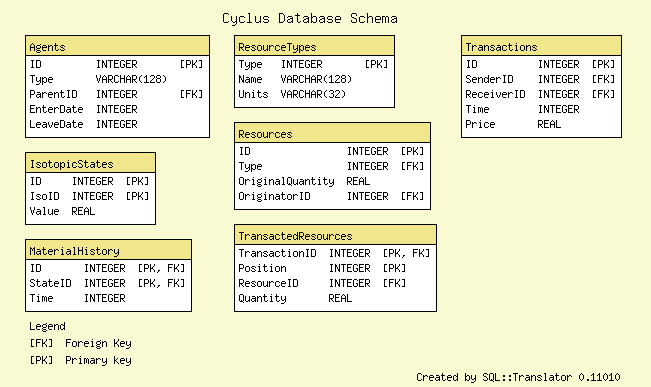
\includegraphics{cycl_schema_bare.png}
\end{quote}

And an example with only the keys connecting each table:
\begin{quote}

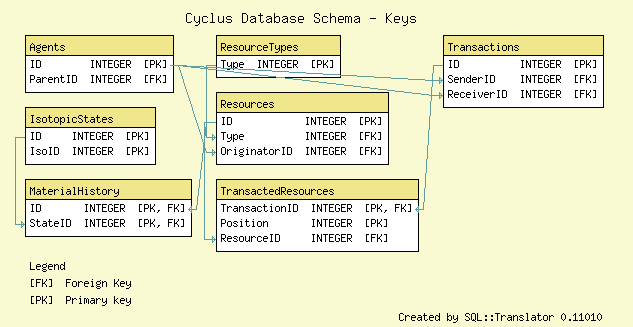
\includegraphics{cycl_schema_keys.png}
\end{quote}

The connections between the full tables are shown below:
\begin{quote}

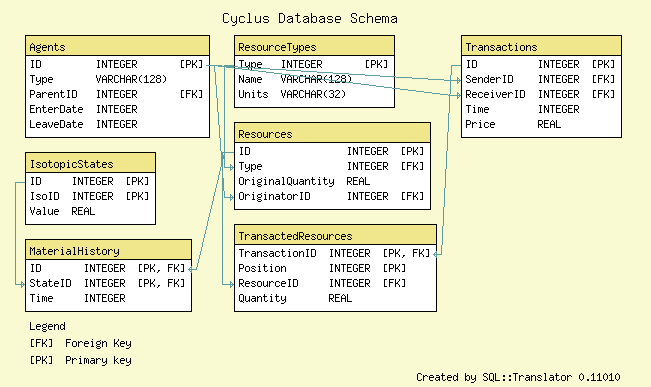
\includegraphics{cycl_schema.png}
\end{quote}


\subsubsection{Use Cases for Cyclus Output Data}
\label{devdoc/output_usecases:use-cases-for-cyclus-output-data}\label{devdoc/output_usecases::doc}

\paragraph{Transaction Data}
\label{devdoc/output_usecases:transaction-data}
The primary \emph{Cyclus} material output data is composed of a log of individual
material transactions.  Each transaction has the following fundamental characteristics:
\begin{itemize}
\item {} 
\textbf{time}: an integer of time steps since the beginning of the simulation

\item {} 
\textbf{sender}: an integer identifying the facility that sent the material

\item {} 
\textbf{recipient}: an integer identifying the facility that received the material

\item {} \begin{description}
\item[{\textbf{manifest}: a vector of material information each containing:}] \leavevmode\begin{itemize}
\item {} \begin{description}
\item[{\textbf{composition vector}: a vector representing the isotopic composition}] \leavevmode
of the material that was transacted

\end{description}

\item {} \begin{description}
\item[{\textbf{quantity}: a double indicating the magnitude of material shipped}] \leavevmode
in this transaction

\end{description}

\end{itemize}

\end{description}

\end{itemize}


\paragraph{Facility Instance Data}
\label{devdoc/output_usecases:facility-instance-data}
The primary \emph{Cyclus} facility output data is composed of a list of
individual facilities.  Each facility have the following fundamental
characteristics:
\begin{itemize}
\item {} 
\textbf{institution}: an integer identifying the institution owning this facility

\item {} 
\textbf{region}: an integer identifying the region in which this facility exists

\item {} 
\textbf{name}: a string that is the name of this instance of the facility

\item {} 
\textbf{prototypeID}: an integer identifying which facility prototype on
which this facility is based.

\item {} 
\textbf{capacity}: a double indicating the capacity of this facility in
some standard units

\end{itemize}

There will also be a table of facility prototypes with generic prototype
information for each:
\begin{itemize}
\item {} 
\textbf{type}: the model used to form this prototype

\item {} 
\textbf{inmarkets}: a list of integers indciating which markets this
prototype receives material from

\item {} 
\textbf{outmarkets}: a list of integers indicating which markets this
prototype ships material to

\end{itemize}


\paragraph{Use Cases}
\label{devdoc/output_usecases:use-cases}
This section will attempt to document a number of primary data
exploration use cases, based on this data.  The two most common modes
are an exploration of the material flows and an exploration of the
facility histories.


\subparagraph{Material flow explorations}
\label{devdoc/output_usecases:material-flow-explorations}
Many material flow explorations would begin by visualizing the
time-dependent material flow between a set of source facilities and a
set of receiving facilities.  The minimum information needed to
generate such a visualization is the population of the two sets of
facilities, and detailed discussion on how to populate these sets is
given below.  Once these sets are defined, the material flow
information can be summed over all the possible transaction pathways
at each time step to generate a single time series of data.  The
following disucussion will identify ways to restrict/limit the
quantity of data represented in such a time series visualization based
primarily on filtering operations for different dimensions of the
material flow data.

It is important to note that single visualizations may contain
multiple time series of data, with a variety of alternative
representations depending on the user's interests.  The following
discussion will consider, in this order:
\begin{enumerate}
\item {} 
the resolution of the time domain,

\item {} 
filtering operations to restrict the data included in a single time series,

\item {} 
application of post-processing functions for alternative engineering responses, and

\item {} 
compartive visualization of multiple time series.

\end{enumerate}


\subparagraph{Time Domain Resolution and Representation}
\label{devdoc/output_usecases:time-domain-resolution-and-representation}
Most simulations are expected to proceed with monthly time steps (this
is user-configurable), probably too fine for meaningful visualization.
The default resolution for such a visualization should be annual flows
of material, requiring a summation operation across non-overlapping
regions of the time domain.  It is likely that a user may want to
interactively change the time domain resolution, possibly interested
in the aggregated solution over time frames that are even coarser than
annual.

It is also likely that users may want to switch between visualizations
of the instantaneous material flow rate within a given step of the
time resolution, and a cumulative material flow, integrating from the
beginning of the simulation to the current step of the time
resolution.

In a related and common time series interaction, users may want to
zoom in and out of regions of the time domain to explore detailed
features.


\subparagraph{Filtering the Sets of Participating Facilities}
\label{devdoc/output_usecases:filtering-the-sets-of-participating-facilities}
Filtering operations will be always be necessary to define the set of
facilities that participate in a given material flow visualization.
The simplest form of such a filter is the selection of an entire
market, thereby selecting all the facilities that participate in that
market.  Beyond that, some other obvious ways to create sets of
facilities for either the source or receiving set are:
\begin{itemize}
\item {} 
choosing individual facilities from a list of existing facilities

\item {} 
choosing individual institutions and therefore including all
facilities owned by that institution

\item {} 
choosing individual regions and therefore including all facilities
operating in that region

\item {} 
choosing a particular facility prototype and therefore including
all facilities based on that prototype

\item {} 
choosing a particular facility module and therefore including all
facilities based on that module

\end{itemize}

The ideal user interface will allow subsets of facilities to be added
and deleted from the ultimate set of facilities using notion of
intersection, union, and negation.

The ideal user interface will also allow a single time series to be
separated into multiple time series (possible displayed in a
comparitive fashion), by selecting a characteristic that defines
subsets of facilities.


\subparagraph{Filtering the Set of Isotopes}
\label{devdoc/output_usecases:filtering-the-set-of-isotopes}
It will also be important to restrict the material flow time series
data by filtering on the set of isotopes that are included in the
material flow data.  There are a small number of standard ways to
define sets of isotopes:
\begin{itemize}
\item {} 
include all isotopes

\item {} 
choose individual chemical elements (e.g. uranium) and thereby
including all the isotopes of that element

\item {} 
choose individual isotopes (e.g. U-235)

\item {} 
choose from predefined meaningful sets of isotopes
(e.g. fission products, actinides, transuranics, fissile isotopes)

\end{itemize}

As with the facility filtering capability, an ideal user interface
will allow subsets of isotopes to be added and deleted from the data
set using notions of intersection, union and negation.

One example of a graph that shows the cumulative makeup of material
in a facility, by isotope, can be found in figure 5.11 of Kyle Oliver's
masters thesis, GeniusV2: Software Design and Mathematical Formulations
For Multi-Region Discrete Nuclear Fuel Cycle Simulation And Analysis.

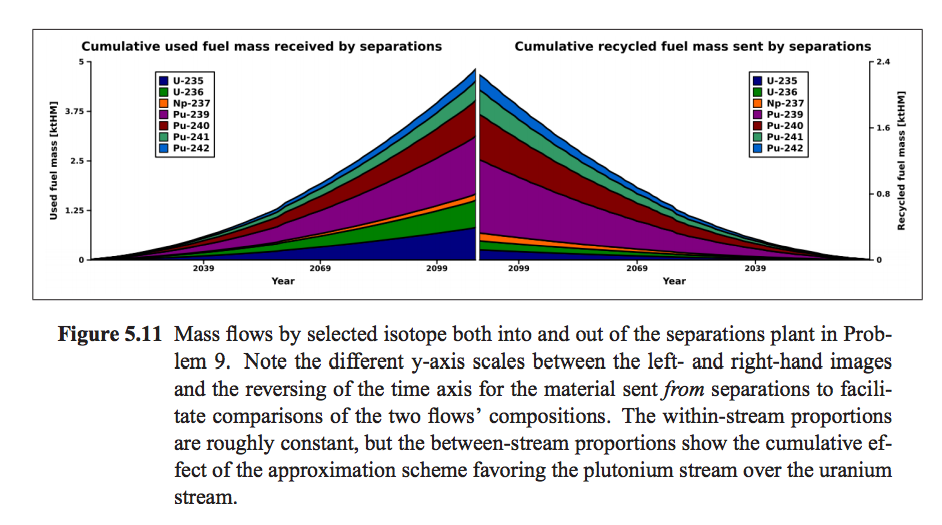
\includegraphics[width=500pt]{cumulative_iso_dist.png}


\subparagraph{Post-processing for Alternative Engineering Responses}
\label{devdoc/output_usecases:post-processing-for-alternative-engineering-responses}
While the fundamental material flows are defined as the raw quantity
of each isotope that is being transacted, there will be a growing set
of transformations that convert these number densities into other
interesting metrics/quantities including:
\begin{itemize}
\item {} 
radiotoxicity

\item {} 
decay heat

\item {} 
waste volume

\item {} 
others-to-be-determined

\end{itemize}

Users will want to apply these transformations, either changing the
metric shown in the primary visualization or cloning the primary
visualization but showing the other metric.


\subparagraph{Workflows for Comparitive Time Series Exploration}
\label{devdoc/output_usecases:workflows-for-comparitive-time-series-exploration}
Once a number of single time series are defined, it will be common to
visualize them on adjacent axes or within the same set of axes.  One
possible workflow is as follows:
\begin{enumerate}
\item {} 
A user selects a market and is immediately shown the
instantaneous material flow through that market over the entire
simulation time domain, with a default time resolution.

\item {} 
A user selects the originating region as a characteristic that
splits the single material flow time series into multiple time
series, each one now defined with a set of source facilities
from a different region.  These time series are shown on the
same axes as a stacked area chart.  The envelope of these now
differentiated time series is identical to the envelope of the
original time series.

\item {} 
The user is then interested in a certain subset of the isotopes,
say the fissile isotopes, and requests that this same material
flow data be filtered to only include those isotopes.  Each of
the material flow time series may (or may not) be reduced as the
set of isotopes it includes is altered.  (Note that while it is
theoretically possible to differentiate by isotope, it may
become difficult to visualize the many different time series
formed by differentiating by facility characteristic and isotope
at the same time.  In some cases, especially where a small
number of isotope subsets are identified, this may be
practical.)

\item {} 
At this point the user may seek a detailed isotopic breakdown of
one of the material flows, either as a time series shown on a
different axis pair, or as a single time step snapshot.  In the
latter case, a variety of options are available to visualize
this, including bar charts, pie charts, tables of data, and
other more advanced representations.  When examining a snapshot,
the linked visualization tool may update constantly as a user
swipes a bar across the time series visualization.

\end{enumerate}

At this point, an ideal user interface may allow users to ``tear-off''
individual time series from the collection of time series into
different axes for further exploration/differentiation in modes
similar to above.


\subparagraph{(Quasi-)Spatial Representation of Material Flows}
\label{devdoc/output_usecases:quasi-spatial-representation-of-material-flows}
Another interesting visualization of this time series data is as an
animated graph representation.  Graph nodes would represent source and
receiving facilties with the connecting arcs somehow indicating the
magnitude of material flow (e.g. line thickness).  The time domain
would be represented by animation.

In some cases, the graphs of two different markets may be shown
together, indicating the connectedness of these graphs through
facilities that participate in both.  Different commodities could be
respresented by different colors, for example.

Such a representation could also be coordinated with the more
traditional time series visualization, in which the graph serves as a
way to select which facilities will be included in the sets for
defining the material flow time series, either by selecting specific
nodes or by selecting specific arcs.

At such a time that geospatial data (or an approximation/surrogate to
this data) is available, this graph visualization could be arranged to
represent the real geospatial locations of facilties.


\subparagraph{Commodity Capacity and Supply/Demand Exploration}
\label{devdoc/output_usecases:commodity-capacity-and-supply-demand-exploration}
Another primary visualization is time series data for installed
capacity of a set of facilities.  Most of the operations discussed
above will be of interest including:
\begin{itemize}
\item {} 
time domain resolution and representation

\item {} 
filtering across different dimensions (although not across an isotope dimension)

\item {} 
applying transformations

\item {} 
comparitive visualization

\end{itemize}

By combining the information about the theoretical capacity with the
information about material transactions, the relationship between
supply and demand can be explored.  (Note that the standardization of
input and output resource buffers within facilities means that
instantaneous transaction flow rates are not always representative of
instantaneous utilization of the available processing capacity.
Access to this information will requires additional output records.)


\subsection{Software Development Aids}
\label{devdoc/main:software-development-aids}

\subsubsection{The \emph{Cyclus} Fuel Cycle Simulator Roadmap}
\label{basics/roadmap:the-cyclus-fuel-cycle-simulator-roadmap}\label{basics/roadmap::doc}
It is expected that external development contributing to the expansion
of the Fuel Cycle Simulator will grow in creative, unpredictable ways
in answer to the needs of the developers.  Moreover, particular use
cases and specific user interests are likely to drive the need for new
capability.

To help direct and inspire development in support of current and anticipated
use cases, the current \emph{Cyclus} development team has identified areas of
essential research areas as well as potential research ideas.


\paragraph{Research Areas}
\label{basics/roadmap:research-areas}
A number of research areas related to \emph{Cyclus} have already been
identified, but others are certainly possible:
\begin{enumerate}
\item {} 
\emph{Cyclus} core infrastructure development

\item {} 
Market model development

\item {} 
Region model development and deployment scenarios

\item {} 
Reactor model development

\item {} 
Separations model development

\item {} 
Geologic repository \& waste form modeling

\item {} 
Graphical interfaces for input and visualization

\item {} 
Social science to determine important metrics and measures

\item {} 
Optimization and sensitivity infrastructure

\item {} 
Transportation

\item {} 
Non-proliferation analysis

\end{enumerate}


\paragraph{Active Projects/Contributors}
\label{basics/roadmap:active-projects-contributors}\begin{itemize}
\item {} \begin{enumerate}
\setcounter{enumi}{20}
\item {} 
Wisconsin-Madison:

\end{enumerate}
\begin{itemize}
\item {} 
\href{http://github.com/cyclus/cyclus}{Cyclus} core infrastructure

\item {} 
\href{http://github.com/cyclus/cycamore}{Cycamore} base module package

\item {} 
\href{http://github.com/katyhuff/cyder}{Cyder} geologic repository modeling

\item {} 
\href{http://github.com/cyclus/cyclopts}{Cyclopts} optimization interface library

\end{itemize}

\item {} \begin{enumerate}
\setcounter{enumi}{20}
\item {} 
Texas at Austin

\end{enumerate}
\begin{itemize}
\item {} 
\href{http://github.com/cyclus/cycic}{Cycic} input control

\end{itemize}

\item {} \begin{enumerate}
\setcounter{enumi}{20}
\item {} 
Utah

\end{enumerate}
\begin{itemize}
\item {} 
\href{http://github.com/cyclus/cyclist}{Cyclist} output visualization

\end{itemize}

\end{itemize}


\paragraph{Potential Research Ideas}
\label{basics/roadmap:potential-research-ideas}
In support of fuel cycle options analysis, modules representing specific
technologies and fuel cycles will contribute significantly to the usefulness of
the cyclus {\hyperref[basics/ecosystem::doc]{\emph{ecosystem}}}. Some specific concepts that have been identified as
potentially versatile models for anticipated fuel cycle modeling goals include a
number of creative Market, Region, Institution, and Facility Models.


\subparagraph{Market Model Ideas}
\label{basics/roadmap:market-model-ideas}
Potential \textbf{Markets} that can be expected to be useful in some anticipated
use cases include contract markets, markets encapsulating fundamental commodity
market theories, markets employing political affinity to make resolution
decisions, markets supporting multipass material routing, and markets that
enable shadow fuel cycles for nuclear proliferation modeling.


\subparagraph{Region Model Ideas}
\label{basics/roadmap:region-model-ideas}
Potential \textbf{Regions} include those supporting political affinity models of
international trade behavior, tax structures, creative growth patterns, political
instabilities capable of causing technology interruption, and international fuel
takeback agreeemnts.


\subparagraph{Institution Model Ideas}
\label{basics/roadmap:institution-model-ideas}
Potentially compelling \textbf{Institutions} might support capacity dispatch logistics
similar to public utility commision behavior or define nuclear growth in the
presence of the growth of nonnuclear energy market share.


\subparagraph{Facility Model Ideas}
\label{basics/roadmap:facility-model-ideas}
Myriad potential \textbf{Facilities} would support the broad {\hyperref[basics/ecosystem::doc]{\emph{ecosystem}}}
of models useful for fuel cycle options analysis. Facility models are the
technical building blocks of Cyclus simulations, and are expected to provide the
modular representation of essential nuclear, chemical, and industrial processes
in fuel cycles of all kinds. Potential fuel cycle technologies of import include
\begin{itemize}
\item {} 
advanced reactors

\item {} 
separations stoichiometry process modules

\item {} 
transportation modules

\item {} 
uranium resource models

\item {} 
nefarious shadow material diversion processes

\item {} 
random facility disruption

\end{itemize}


\subparagraph{Full Simulation Scale Contributions}
\label{basics/roadmap:full-simulation-scale-contributions}
Additional simulation-level features envisioned to become useful in the near
term for optimization, economic, and strategic use cases include :
\begin{itemize}
\item {} 
external multi-variable optimization demonstration

\item {} 
objective functions for assessing overall simulation performance (e.g. economic)

\item {} 
investigation of impact of varying module fidelity

\item {} 
implementations of relevant simulation use cases, benchmarking cases, etc.

\end{itemize}


\subsubsection{Guide for Contributing to Cyclus}
\label{devdoc/contributing_to_cyclus:guide-for-contributing-to-cyclus}\label{devdoc/contributing_to_cyclus::doc}
\emph{Cyclus} has a number of projects under its umbrella.
The core \emph{Cyclus} project repository is located at
\href{http://github.com/cyclus/cyclus}{http://github.com/cyclus/cyclus}. Additional projects found at
\href{http://github.com/cyclus}{http://github.com/cyclus} include :
\begin{itemize}
\item {} 
Cycamore, the cyclus additional modules repository

\item {} 
Cyclopts, the cyclus optimization library

\item {} 
Cycic, the cyclus input controller

\item {} 
and more to come.

\end{itemize}

Although you do not have to register with github to
download and edit the code, if you desire your work to be integrated into the
cyclus mainline of development \emph{you must fork the cyclus core repository into
your own github account and submit `Pull Requests'}. {\hyperref[devdoc/get_and_build::doc]{\emph{Here is a tutorial on
getting and building cyclus.}}}


\paragraph{Working on a Topic}
\label{devdoc/contributing_to_cyclus:working-on-a-topic}
\emph{Note that ``upstream'' repository refers to the primary {}`cyclus/cyclus{}` repository.}

You may find or create an issue report in a \emph{Cyclus} repository that you would like
to solve.

You'll first need to fork your repository and create a branch for the topic you'd
like you solve. As you do your development, push only to your own fork. Make a
pull request to the upstream repository (usually the ``develop'' branch) only after:
\begin{itemize}
\item {} 
You have pulled the latest changes from the upstream repository.

\item {} 
You have completed a logical set of changes.

\item {} 
Cyclus compiles with no errors.

\item {} 
All tests pass.

\item {} 
Cyclus input files run as expected.

\item {} 
Your code has been reviewed by another developer.

\end{itemize}

Code from the ``develop'' branch generally must pass even more rigorous checks
before being integrated into the ``master'' branch. Hotfixes would be a
possible exception to this.


\paragraph{Keeping Your Fork Up To Date}
\label{devdoc/contributing_to_cyclus:keeping-your-fork-up-to-date}\begin{itemize}
\item {} 
Use a branching workflow similar to the one described at
\href{http://progit.org/book/ch3-4.html}{http://progit.org/book/ch3-4.html}.

\item {} 
The ``develop'' branch is how cyclus developers will share (generally compilable) progress
when we are not yet ready for the code to become `production'.

\item {} 
Keep your own ``master'' and ``develop'' branches in sync with the upstream repository's
``master'' and ``develop'' branches. The master branch should always be the `stable'
or `production' release of cyclus.
\begin{itemize}
\item {} 
Pull the most recent history from the upstream repository ``master''
and/or ``develop'' branches before you merge changes into your
corresponding local branch. Consider doing a rebase pull instead of
a regular pull or `fetch and merge'.  For example:

\begin{Verbatim}[commandchars=\\\{\}]
git checkout develop
git pull --rebase upstream develop
\end{Verbatim}

\end{itemize}

\item {} 
As you do development on topic branches in your own fork, consider rebasing
the topic branch onto the ``master'' and/or ``develop''  branches after \emph{pulls} from the upstream
repository rather than merging the pulled changes into your branch.  This
will help maintain a more linear (and clean) history.
\emph{Please see caution about rebasing below}.  For example:

\begin{Verbatim}[commandchars=\\\{\}]
git checkout [your topic branch]
git rebase develop
\end{Verbatim}

\end{itemize}


\paragraph{Passing Tests}
\label{devdoc/contributing_to_cyclus:passing-tests}
To check that your branch passes the tests, you must build and install your topic
branch and then run the tests built during that process.

For the cyclus core, the tests are run using the CyclusUnitTestDriver (at the moment,
\code{{}`make test{}`} is insufficient). For example

\begin{Verbatim}[commandchars=\\\{\}]
mkdir build
mkdir install
cd build
cmake ../src -DCMAKE\_INSTALL\_PREFIX=../install
make
make install
../install/cyclus/bin/CyclusUnitTestDriver
\end{Verbatim}

The cycamore, the additional modules repository, the tests are run in an exactly
analogous way, but using the CycamoreUnitTestDriver. For example

\begin{Verbatim}[commandchars=\\\{\}]
mkdir build
mkdir install
cd build
cmake ../src -DCMAKE\_INSTALL\_PREFIX=../install
make
make install
../install/cycamore/bin/CycamoreUnitTestDriver
\end{Verbatim}

In addition to the CycamoreUnitTestDriver, a suite of input files can be run and
tested using the run\_inputs.py script that is configured, built, and installed
with Cycamore. It relies on the input files that are part of your Cycamore
repository, and only succeeds for input files that are correct (some may have
known issues. See the issue list in cycamore for details.) To run the example
input files,

\begin{Verbatim}[commandchars=\\\{\}]
python ../install/cycamore/bin/run\_inputs.py
\end{Verbatim}


\paragraph{Making a Pull Request}
\label{devdoc/contributing_to_cyclus:making-a-pull-request}
When you are ready to move changes from one of your topic branches into the
``develop'' branch, it must be reviewed and accepted by another developer.
\begin{itemize}
\item {} 
You may want to review this \href{https://help.github.com/articles/using-pull-requests/}{tutorial}
before you make a pull request to the develop branch.

\end{itemize}

Sometimes, your pull request will be closed by the reviewer until further
changes are made to appease the reviewer's concerns. This may be frustrating,
but please act rationally, discuss the issues on the github space made for your
pull request, consult the \emph{style guide \textless{}style\_guide\textgreater{}},
email the developer listhost for further advice, and make changes to your topic branch
accordingly. The pull request will be updated with those changes when you push them
to your fork.  When you think your request is ready for another review, you can
reopen the review yourself with the button made available to you.


\paragraph{Reviewing a Pull Request}
\label{devdoc/contributing_to_cyclus:reviewing-a-pull-request}\begin{itemize}
\item {} 
Build, install, and test it. If you have added the remmote repository as
a remote you can check it out and merge it with the current develop
branch thusly,

\begin{Verbatim}[commandchars=\\\{\}]
git checkout -b remote\_name/branch\_name
git merge develop
\end{Verbatim}

\item {} 
Look over the code.
\begin{itemize}
\item {} 
Check that it meets {\hyperref[devdoc/style_guide::doc]{\emph{our style guidelines}}}.

\item {} 
Make inline review comments concerning improvements.

\end{itemize}

\item {} 
Accept the Pull Request
\begin{itemize}
\item {} 
In general, \textbf{every commit} (notice this is not `every push') to the
``develop'' and ``master'' branches should compile and pass tests. This
is guaranteed by using a NON-fast-forward merge during the pull request
acceptance process.

\item {} 
The green ``Merge Pull Request'' button does a non-fast-forward merge by
default. However, if that button is unavailable, you've made minor
local changes to the pulled branch, or you just want to do it from the
command line, make sure your merge is a non-fast-forward merge. For example:

\begin{Verbatim}[commandchars=\\\{\}]
git checkout develop
git merge --no-ff remote\_name/branch\_name -m "A message""
\end{Verbatim}

\end{itemize}

\end{itemize}


\paragraph{See also}
\label{devdoc/contributing_to_cyclus:see-also}
A good description of a git workflow with good graphics is available at
\href{http://nvie.com/posts/a-successful-git-branching-model/}{http://nvie.com/posts/a-successful-git-branching-model/}


\subsubsection{Developing Models For Cyclus}
\label{devdoc/make-models/main::doc}\label{devdoc/make-models/main:developing-models-for-cyclus}

\paragraph{Introduction}
\label{devdoc/make-models/main:introduction}
\emph{Cyclus} employs a Region-Institution-Facility hierarchy in simulations. Additionally,
Resources are traded amonst the simulation agents via Markets. The instructions here will
describe both how to add specific modules within those types, as well as how to extend this to
other types of loadable modules.


\paragraph{Creating New Models of the Existing Types}
\label{devdoc/make-models/main:creating-new-models-of-the-existing-types}
For each type of model (i.e. Market, Facility, Institution, or Region), a set of stub
files are available as skeletons for the new models.  When creating a new model, it is important that all the
functionality defined in these files remains in the final model definition. A
step by step example of producing a new model from the existing stubs can be
found in the {\hyperref[devdoc/make-models/toaster::doc]{\emph{Model Devlopment Example : ToasterFacility}}}.


\paragraph{Model Initialization and Creation}
\label{devdoc/make-models/main:model-initialization-and-creation}
The Cyclus simulation environment has a number of fundamental aspects regarding
model creation:
\begin{itemize}
\item {} 
Models in Cyclus follow a parent-child paradigm, i.e. a model has one parent and
may have many children. The parent-child relationship can be thought of as
ownership.

\item {} 
Models in Cyclus are either Prototypes (templates) or Models (participants)
\begin{itemize}
\item {} 
A Model becomes a Prototype (template) after initialization

\item {} 
A Model becomes a Model (paticipant) after its \emph{parent is set} via the
setParent() method defined in Model.h.

\item {} 
All Models start as Prototypes and become Models

\end{itemize}

\end{itemize}

A Model can have many possible initilization-related methods; however, every Model
has \emph{at least} a method named init(). In init(), any and all publicly accesible
members must be initialized. Should such a member attempt to be accessed when not
initialized, a segmentation fault will occur. An example from the BuildRegion class
is shown:

\begin{Verbatim}[commandchars=\\\{\}]
\PYG{c+c1}{//- - - - - - - - - - - - - - - - - - - - - - - - - - - - - - - - - - -}
\PYG{k+kt}{void} \PYG{n}{BuildRegion}\PYG{o}{:}\PYG{o}{:}\PYG{n}{init}\PYG{p}{(}\PYG{p}{)} \PYG{p}{\PYGZob{}}
  \PYG{n}{prototypeOrders\PYGZus{}} \PYG{o}{=} \PYG{k}{new} \PYG{n}{PrototypeOrders}\PYG{p}{(}\PYG{p}{)}\PYG{p}{;}
  \PYG{n}{builders\PYGZus{}} \PYG{o}{=} \PYG{k}{new} \PYG{n}{map}\PYG{o}{\textless{}}\PYG{n}{Model}\PYG{o}{*}\PYG{p}{,} \PYG{n}{std}\PYG{o}{:}\PYG{o}{:}\PYG{n}{list}\PYG{o}{\textless{}}\PYG{n}{Model}\PYG{o}{*}\PYG{o}{\textgreater{}}\PYG{o}{*}\PYG{o}{\textgreater{}}\PYG{p}{(}\PYG{p}{)}\PYG{p}{;}
\PYG{p}{\PYGZcb{}}
\end{Verbatim}

Note that prototypeOrders and builders are defined in the header file and accessed
via public methods.

In order to maintain clarity and flexibility, initialization methods are as
modularized as possible. The more involved a Model's initialization process,
the more benefit is gained from modularity. As a concrete example, let us examine
the RegionModel base class's xml initialization process.

\begin{Verbatim}[commandchars=\\\{\}]
\PYG{c+c1}{//- - - - - - - - - - - - - - - - - - - - - - - - - - - - - - - - - - -}
\PYG{k+kt}{void} \PYG{n}{RegionModel}\PYG{o}{:}\PYG{o}{:}\PYG{n}{init}\PYG{p}{(}\PYG{n}{xmlNodePtr} \PYG{n}{cur}\PYG{p}{)} \PYG{p}{\PYGZob{}}
  \PYG{n}{RegionModel}\PYG{o}{:}\PYG{o}{:}\PYG{n}{init}\PYG{p}{(}\PYG{p}{)}\PYG{p}{;} \PYG{c+c1}{// init any RegionModel members}
  \PYG{n}{Model}\PYG{o}{:}\PYG{o}{:}\PYG{n}{init}\PYG{p}{(}\PYG{n}{cur}\PYG{p}{)}\PYG{p}{;} \PYG{c+c1}{// name and model\PYGZus{}impl}
  \PYG{n}{RegionModel}\PYG{o}{:}\PYG{o}{:}\PYG{n}{initAllowedFacilities}\PYG{p}{(}\PYG{n}{cur}\PYG{p}{)}\PYG{p}{;} \PYG{c+c1}{// allowedFacilities}
  \PYG{n}{RegionModel}\PYG{o}{:}\PYG{o}{:}\PYG{n}{initSimInteraction}\PYG{p}{(}\PYG{k}{this}\PYG{p}{)}\PYG{p}{;} \PYG{c+c1}{// parent and tick listener, model 'born'}
  \PYG{n}{RegionModel}\PYG{o}{:}\PYG{o}{:}\PYG{n}{initChildren}\PYG{p}{(}\PYG{n}{cur}\PYG{p}{)}\PYG{p}{;} \PYG{c+c1}{// children-\textgreater{}setParent}
\PYG{p}{\PYGZcb{}}
\end{Verbatim}

Here, each major step is given its own function. This allows developers who base
their models on RegionModel to customize their own xml init method, as shown
in the BuildRegion class:

\begin{Verbatim}[commandchars=\\\{\}]
\PYG{c+c1}{//- - - - - - - - - - - - - - - - - - - - - - - - - - - - - - - - - - -}
\PYG{k+kt}{void} \PYG{n}{BuildRegion}\PYG{o}{:}\PYG{o}{:}\PYG{n}{init}\PYG{p}{(}\PYG{n}{xmlNodePtr} \PYG{n}{cur}\PYG{p}{)} \PYG{p}{\PYGZob{}}
  \PYG{c+c1}{// non xml inits}
  \PYG{n}{BuildRegion}\PYG{o}{:}\PYG{o}{:}\PYG{n}{init}\PYG{p}{(}\PYG{p}{)}\PYG{p}{;}
  \PYG{n}{RegionModel}\PYG{o}{:}\PYG{o}{:}\PYG{n}{init}\PYG{p}{(}\PYG{p}{)}\PYG{p}{;} \PYG{c+c1}{// we never explicitly call RegionModel::init(cur)}
  \PYG{c+c1}{// xml inits}
  \PYG{n}{Model}\PYG{o}{:}\PYG{o}{:}\PYG{n}{init}\PYG{p}{(}\PYG{n}{cur}\PYG{p}{)}\PYG{p}{;} \PYG{c+c1}{// name\PYGZus{} and model\PYGZus{}impl\PYGZus{}}
  \PYG{n}{RegionModel}\PYG{o}{:}\PYG{o}{:}\PYG{n}{initAllowedFacilities}\PYG{p}{(}\PYG{n}{cur}\PYG{p}{)}\PYG{p}{;} \PYG{c+c1}{// allowedFacilities\PYGZus{}}

  \PYG{c+c1}{// get path to this model}
  \PYG{n}{xmlNodePtr} \PYG{n}{model\PYGZus{}cur} \PYG{o}{=}
    \PYG{n}{XMLinput}\PYG{o}{-}\PYG{o}{\textgreater{}}\PYG{n}{get\PYGZus{}xpath\PYGZus{}element}\PYG{p}{(}\PYG{n}{cur}\PYG{p}{,}\PYG{l+s}{"}\PYG{l+s}{model/BuildRegion}\PYG{l+s}{"}\PYG{p}{)}\PYG{p}{;}

  \PYG{c+c1}{// populate orders for each prototype}
  \PYG{n}{xmlNodeSetPtr} \PYG{n}{prototype\PYGZus{}nodes} \PYG{o}{=}
    \PYG{n}{XMLinput}\PYG{o}{-}\PYG{o}{\textgreater{}}\PYG{n}{get\PYGZus{}xpath\PYGZus{}elements}\PYG{p}{(}\PYG{n}{model\PYGZus{}cur}\PYG{p}{,}\PYG{l+s}{"}\PYG{l+s}{prototyperequirement}\PYG{l+s}{"}\PYG{p}{)}\PYG{p}{;}
  \PYG{k}{for} \PYG{p}{(}\PYG{k+kt}{int} \PYG{n}{i}\PYG{o}{=}\PYG{l+m+mi}{0}\PYG{p}{;}\PYG{n}{i}\PYG{o}{\textless{}}\PYG{n}{prototype\PYGZus{}nodes}\PYG{o}{-}\PYG{o}{\textgreater{}}\PYG{n}{nodeNr}\PYG{p}{;}\PYG{n}{i}\PYG{o}{+}\PYG{o}{+}\PYG{p}{)}\PYG{p}{\PYGZob{}}
    \PYG{n}{populateOrders}\PYG{p}{(}\PYG{n}{prototype\PYGZus{}nodes}\PYG{o}{-}\PYG{o}{\textgreater{}}\PYG{n}{nodeTab}\PYG{p}{[}\PYG{n}{i}\PYG{p}{]}\PYG{p}{)}\PYG{p}{;}
  \PYG{p}{\PYGZcb{}}
  \PYG{n}{sortOrders}\PYG{p}{(}\PYG{p}{)}\PYG{p}{;}

  \PYG{c+c1}{// parent\PYGZus{} and tick listener, model 'born'}
  \PYG{n}{RegionModel}\PYG{o}{:}\PYG{o}{:}\PYG{n}{initSimInteraction}\PYG{p}{(}\PYG{k}{this}\PYG{p}{)}\PYG{p}{;}
  \PYG{c+c1}{// children-\textgreater{}setParent, requires init()}
  \PYG{n}{RegionModel}\PYG{o}{:}\PYG{o}{:}\PYG{n}{initChildren}\PYG{p}{(}\PYG{n}{cur}\PYG{p}{)}\PYG{p}{;}

  \PYG{c+c1}{// populate the list of builders}
  \PYG{n}{populateBuilders}\PYG{p}{(}\PYG{p}{)}\PYG{p}{;}
\PYG{p}{\PYGZcb{}}\PYG{p}{;}
\end{Verbatim}


\paragraph{Creating Specific Model Types}
\label{devdoc/make-models/main:creating-specific-model-types}
For further details about creating new models of particular types, consult the
Model-specific reference:


\subparagraph{Developing Facility Models}
\label{devdoc/make-models/facility::doc}\label{devdoc/make-models/facility:developing-facility-models}

\subparagraph{Details}
\label{devdoc/make-models/facility:details}
In addition to inheriting from the main dynamic loading base class \emph{Model}, all
FacilityModel models also inherit from \emph{Communicator}.

A FacilityModel is one of the primary actors in the \emph{Cyclus} system.  All
offers and requests originate at an instance of a FacilityModel and all
shipments are executed by an instance of a FacilityModel.

While running, \emph{Cyclus} will use a FacilityModel in two ways.  First, it will
read user input to define a template instance of a FacilityModel.  A choice of
a FacilityModel model combined with some distinct set of parameters for that
model results in a facility that is available for deployment by an InstModel
institution if allowed by that institution's RegionModel region.  Second,
\emph{Cyclus} will create copies of the FacilityModel facilities as they are
deployed by the institutions.  For this reason, the FacilityModel class defines
a data member \emph{fac\_name} that is the name of the individual deployed facility.

All FacilityModel models should know which set of Commodity objects they trade
and/or which MarketModel markets they participate in.  Each FacilityModel model
should implement a method named \emph{sendMessages} to generate offer and request
messages to send to their markets and methods named \emph{sendMaterial} and
\emph{receiveMaterial} to process shipment messages that originate with their
markets.


\subparagraph{Developing Institution Models}
\label{devdoc/make-models/institution::doc}\label{devdoc/make-models/institution:developing-institution-models}

\subparagraph{Details}
\label{devdoc/make-models/institution:details}
In addition to inheriting from the main dynamic loading base class \emph{Model}, all
InstModel models also inherit from \emph{Communicator}.

A InstModel's primary function is to
\begin{itemize}
\item {} 
refer to the set of facilities operating in this institution

\end{itemize}

All InstModel models may also implement a reciveMessage function if messages
need to be amended by the institution before being sent up to the region or
down to the facility. This is a virtual (but not pure virtual) function, so
implementation is optional. Default behavior is to ignore the message.

InstModel models are sent a tick and tock signal at the beginning and end of
each month, respectively. Monthly tasks, such as facility deployment or
bookkeeping should be undertaken within the handleTick and handleTock
functions. These are virtual (but not pure virtual), so implementation of these
functions is optional.
\begin{quote}

\emph{The InstModel model type is not yet stable and additional interface and
data members are expected to be added.}
\end{quote}


\subparagraph{Developing Region Models}
\label{devdoc/make-models/region:developing-region-models}\label{devdoc/make-models/region::doc}

\subparagraph{Details}
\label{devdoc/make-models/region:details}
In addition to inheriting from the main dynamic loading base class \emph{Model}, all
RegionModel models also inherit from \emph{Communicator}.

A RegionModel's primary functions are to
\begin{itemize}
\item {} 
contain a set of institutions that operate in this region

\item {} 
define a set of allowed facilities for those institutions

\item {} 
Schedule the deployment of facilities by either
\begin{enumerate}
\item {} 
Determining when new facilities need to be built, or

\item {} 
deferring to an InstModel to make this determination.

\end{enumerate}

\item {} 
Manage the deployment of facilities by interacting with the Institutions to select a specific facility type and facility parameters

\item {} 
Passing material offers/requests between a prescribed market and related facilities.

\end{itemize}

All RegionModel models have an STL \emph{set} of pointers to the \emph{Model} instances
that represent the allowed FacilityModel facilities. and an STL \emph{vector} of
pointers to the \emph{Model} instances that represent the contained InstModel
institutions.

All RegionModel models may also implement a reciveMessage function if messages
need to be amended by the region before being sent up to the market or down to
the institution. This is a virtual (but not pure virtual) function, so
implementation is optional. Default behavior is to ignore the message.

RegionModel models are sent a tick and tock signal at the beginning and end of
each month, respectively. Monthly tasks, such as facility deployment or
bookkeeping should be undertaken within the handleTick and handleTock
functions. These are virtual (but not pure virtual), so implementation of these
functions is optional.


\subparagraph{To Do}
\label{devdoc/make-models/region:to-do}
RegionModel models should be the mechanism for implementing demand growth.
Different implementations of RegionModel models might implement different ways
to model that growth. (Or is this all pre-processing?)


\subparagraph{Developing Market Models}
\label{devdoc/make-models/market::doc}\label{devdoc/make-models/market:developing-market-models}

\subparagraph{Details}
\label{devdoc/make-models/market:details}
In addition to inheriting from the main dynamic loading base class \emph{Model}, all
MarketModel models also inherit from \emph{Communicator}.

A MarketModel's primary function is to
\begin{itemize}
\item {} 
receive offers and requests from facilities,

\item {} 
\emph{resolve} the market by matching those offers and requests

\item {} 
generate/execute a set of orders for shipments of material between
facilities that results from resolving the market

\end{itemize}

Therefore, all MarketModel models should implement their own version of
\emph{receiveOfferRequest} that registers incoming offers and requests in a way that
is appropriate for this market implementation.  All MarketModel models must
also implement their own version of \emph{resolve}.

All MarketModel models have an STL \emph{set} of pointers to the \emph{OfferRequest}
messages that have arrived and an STL \emph{deque} of pointers to the \emph{Shipment}
messages that it is generating.  MarketModel models are also free to have
additional storage modes for \emph{OfferRequest} messages or \emph{Shipment} messages
that facilitates the operation of that particular MarketModel paradigm.


\subparagraph{Model Devlopment Example : ToasterFacility}
\label{devdoc/make-models/toaster:model-devlopment-example-toasterfacility}\label{devdoc/make-models/toaster::doc}

\subparagraph{Introduction}
\label{devdoc/make-models/toaster:introduction}
The instructions here will use a fictional example (a Toaster) to describe the
specific steps to take in order to easily create a custom module suitable for
integration with the Cyclus framework. The module pursued here is a Facility
type module which converts a \emph{bread} Material Resource into a \emph{toast} Material
Resource. In order to do this,

For each type of model (i.e. Market, Facility, Institution, or Region), a set of
stub files are available as skeletons for the new models.  When creating a new
model, it is important that all the functionality defined in these files remains
in the final model definition.


\subparagraph{Forking the cycstub Repository}
\label{devdoc/make-models/toaster:forking-the-cycstub-repository}
Full instructions for Forking the cycstub repository can be found on \href{https://github.com/cyclus/cycstub}{its main
page.}

Once you have forked, cloned, and configured the cycstub repository, you'll be
able to use the stub templates you've downloaded to create your toaster
facility (for example).


\subparagraph{Beginning With a Stub Template}
\label{devdoc/make-models/toaster:beginning-with-a-stub-template}
To create a new model, e.g. a new FacilityModel of type ToasterFacility:
\begin{enumerate}
\item {} 
In the cycstub clone, rename the StubFacility directory and all of the files
it contains to a new directory called ToasterFacility.

\item {} 
Rename the Stub* files within that directory to corresponding Toaster* files.
(That is, rename StubFacility.cpp to ToasterFacility.cpp, etc.)

\item {} 
Search instances of \emph{Stub} and \emph{STUB} within those files and replace them
with \emph{Toaster} and \emph{TOASTER}. That is, code such as:

\end{enumerate}

\begin{Verbatim}[commandchars=\\\{\}]
\PYG{c+cp}{// StubFacility.h}
\PYG{c+cp}{\PYGZsh{}}\PYG{c+cp}{if !defined(\PYGZus{}STUBFACILITY\PYGZus{}H)}
\PYG{c+cp}{\PYGZsh{}}\PYG{c+cp}{define \PYGZus{}STUBFACILITY\PYGZus{}H}

\PYG{c+cp}{\PYGZsh{}}\PYG{c+cp}{include "Logger.h"}
\PYG{c+cp}{\PYGZsh{}}\PYG{c+cp}{include "FacilityModel.h"}

\PYG{k}{class} \PYG{n+nc}{StubFacility} \PYG{o}{:} \PYG{k}{public} \PYG{n}{FacilityModel}  \PYG{c+c1}{// ...}
\end{Verbatim}

would become :

\begin{Verbatim}[commandchars=\\\{\}]
\PYG{c+cp}{// ToasterFacility.h}
\PYG{c+cp}{\PYGZsh{}}\PYG{c+cp}{if !defined(\PYGZus{}TOASTERFACILITY\PYGZus{}H)}
\PYG{c+cp}{\PYGZsh{}}\PYG{c+cp}{define \PYGZus{}TOASTERFACILITY\PYGZus{}H}

\PYG{c+cp}{\PYGZsh{}}\PYG{c+cp}{include "Logger.h"}
\PYG{c+cp}{\PYGZsh{}}\PYG{c+cp}{include "FacilityModel.h"}

\PYG{k}{class} \PYG{n+nc}{ToasterFacility} \PYG{o}{:} \PYG{k}{public} \PYG{n}{FacilityModel}  \PYG{c+c1}{// ...}
\end{Verbatim}


\subparagraph{Customization of the Relax-NG Grammar}
\label{devdoc/make-models/toaster:customization-of-the-relax-ng-grammar}
The parameters that define a Toaster are :
\begin{itemize}
\item {} 
\textbf{nSlices} :  How many slices it can toast at once {[} integer number of slices
{]}

\item {} 
\textbf{toastiness} : How toasted they become {[} light, golden, dark, burnt {]}

\item {} 
\textbf{rate} : How long it takes to toast a set of slices {[} minutes {]}

\item {} 
\textbf{incommodity} : The commodity market in which slices of bread are traded in
this simulation {[} a string {]}

\item {} 
\textbf{outcommodity} : The commodity market in which toasted bread is traded in
this simulation {[} a string {]}

\end{itemize}

To tell the cyclus framework that this is the necessary information to define a
ToasterFacility, we include a Relax-NG grammar file. The stub looks like :

\begin{Verbatim}[commandchars=\\\{\}]
\PYG{n+nt}{\textless{}grammar} \PYG{n+na}{xmlns=}\PYG{l+s}{"http://relaxng.org/ns/structure/1.0"}
\PYG{n+na}{datatypeLibrary=}\PYG{l+s}{"http://www.w3.org/2001/XMLSchema-datatypes"}\PYG{n+nt}{\textgreater{}}

\PYG{n+nt}{\textless{}define} \PYG{n+na}{name=}\PYG{l+s}{"ToasterFacility"}\PYG{n+nt}{\textgreater{}}
  \PYG{n+nt}{\textless{}element} \PYG{n+na}{name=}\PYG{l+s}{"ToasterFacility"}\PYG{n+nt}{\textgreater{}}
    \PYG{n+nt}{\textless{}ref} \PYG{n+na}{name=}\PYG{l+s}{"incommodity"}\PYG{n+nt}{/\textgreater{}}
     \PYG{n+nt}{\textless{}oneOrMore}\PYG{n+nt}{\textgreater{}}
       \PYG{n+nt}{\textless{}ref} \PYG{n+na}{name=}\PYG{l+s}{"outcommodity"}\PYG{n+nt}{/\textgreater{}}
     \PYG{n+nt}{\textless{}/oneOrMore\textgreater{}}
    \PYG{n+nt}{\textless{}/element\textgreater{}}
 \PYG{n+nt}{\textless{}/define\textgreater{}}
\end{Verbatim}

To customize it to include the parameters above, change it to look like :

\begin{Verbatim}[commandchars=\\\{\}]
\PYG{n+nt}{\textless{}grammar} \PYG{n+na}{xmlns=}\PYG{l+s}{"http://relaxng.org/ns/structure/1.0"}
\PYG{n+na}{datatypeLibrary=}\PYG{l+s}{"http://www.w3.org/2001/XMLSchema-datatypes"}\PYG{n+nt}{\textgreater{}}

\PYG{n+nt}{\textless{}define} \PYG{n+na}{name=}\PYG{l+s}{"ToasterFacility"}\PYG{n+nt}{\textgreater{}}
  \PYG{n+nt}{\textless{}element} \PYG{n+na}{name=}\PYG{l+s}{"ToasterFacility"}\PYG{n+nt}{\textgreater{}}
    \PYG{n+nt}{\textless{}element} \PYG{n+na}{name=}\PYG{l+s}{"nSlices"}\PYG{n+nt}{\textgreater{}}
      \PYG{n+nt}{\textless{}data} \PYG{n+na}{type=}\PYG{l+s}{"nonNegativeInteger"}\PYG{n+nt}{/\textgreater{}}
      \PYG{n+nt}{\textless{}/element\textgreater{}}
    \PYG{n+nt}{\textless{}element} \PYG{n+na}{name=}\PYG{l+s}{"toastiness"}\PYG{n+nt}{\textgreater{}}
      \PYG{n+nt}{\textless{}data} \PYG{n+na}{type=}\PYG{l+s}{"string"}\PYG{n+nt}{/\textgreater{}}
      \PYG{n+nt}{\textless{}/element\textgreater{}}
    \PYG{n+nt}{\textless{}element} \PYG{n+na}{name=}\PYG{l+s}{"rate"}\PYG{n+nt}{\textgreater{}}
      \PYG{n+nt}{\textless{}data} \PYG{n+na}{type=}\PYG{l+s}{"double"}\PYG{n+nt}{/\textgreater{}}
      \PYG{n+nt}{\textless{}/element\textgreater{}}
    \PYG{n+nt}{\textless{}ref} \PYG{n+na}{name=}\PYG{l+s}{"incommodity"}\PYG{n+nt}{/\textgreater{}}
    \PYG{n+nt}{\textless{}ref} \PYG{n+na}{name=}\PYG{l+s}{"outcommodity"}\PYG{n+nt}{/\textgreater{}}
    \PYG{n+nt}{\textless{}/element\textgreater{}}
 \PYG{n+nt}{\textless{}/define\textgreater{}}
\end{Verbatim}

There are a few things to notice here.
\begin{itemize}
\item {} 
The incommodity and outcommodity elements are already defined. Since these are
common module parameters, they can be used by reference (note the ref syntax)
in any rng file within the simulation.  * The data types of the parameters are
defined by the datatypeLibrary referenced in the top line. The documentation
for this datatype library can be found at the url. This is provided only for
convenience, and allows the XML parser to check the datatype of user input.

\item {} 
The toastiness parameter is passed as a string. This means that the input
error checking, string interpretation, and other parsing that must be done to
ensure that the value provided is within the available (light, golden, dark,
burnt) options must be done in the initialization function on the c++ side.
Though this parameter could have been defined in other ways, thisi is a good
example of how to arrage to do the input parsing task outside of xml. \textbf{Note
that such a string parameter could also be used to provide the name of another
input file that helps define a module. The interpretation, again, would have
to be done on the c++ side}

\end{itemize}


\subparagraph{Customization of the Documentation Comments}
\label{devdoc/make-models/toaster:customization-of-the-documentation-comments}
To build documentation of your module into the doxygen documentation you or your
users build locally, your code must contain informative, Doxygen style comments
to describe the classes and functions that define your module. More details of
this are discussed in the style guide, but the Stub files give a good begining.

For our ToasterFacility, the ToasterFacility.h file, for instance, has a section
that looks like :

\begin{Verbatim}[commandchars=\\\{\}]
\PYG{c+cp}{// ToasterFacility.h}
\PYG{c+cp}{\PYGZsh{}}\PYG{c+cp}{if !defined(\PYGZus{}TOASTERFACILITY\PYGZus{}H)}
\PYG{c+cp}{\PYGZsh{}}\PYG{c+cp}{define \PYGZus{}TOASTERFACILITY\PYGZus{}H}

\PYG{c+cp}{\PYGZsh{}}\PYG{c+cp}{include "Logger.h"}
\PYG{c+cp}{\PYGZsh{}}\PYG{c+cp}{include "FacilityModel.h"}

\PYG{c+cm}{/*!}
\PYG{c+cm}{  @class ToasterFacility}

\PYG{c+cm}{  @brief This FacilityModel is intended as a skeleton to guide the}
\PYG{c+cm}{  implementation of new FacilityModel models.}

\PYG{c+cm}{  The ToasterFacility class inherits from the FacilityModel class and is}
\PYG{c+cm}{  dynamically loaded by the Model class when requested.}

\PYG{c+cm}{  @section intro Introduction}
\PYG{c+cm}{  Place an introduction to the model here.}

\PYG{c+cm}{  @section modelparams Model Parameters}
\PYG{c+cm}{  Place a description of the required input parameters which define the model}
\PYG{c+cm}{  implementation.}

\PYG{c+cm}{  @section optionalparams Optional Parameters}
\PYG{c+cm}{  Place a description of the optional input parameters to define the model}
\PYG{c+cm}{  implementation.}

\PYG{c+cm}{  @section detailed Detailed Behavior}
\PYG{c+cm}{  Place a description of the detailed behavior of the model. Consider}
\PYG{c+cm}{  describing the behavior at the tick and tock as well as the behavior upon}
\PYG{c+cm}{  sending and}
\PYG{c+cm}{  receiving materials and messages.}
\PYG{c+cm}{  !*/}
\end{Verbatim}

This should looke more like :

\begin{Verbatim}[commandchars=\\\{\}]
\PYG{c+cp}{// ToasterFacility.h}
\PYG{c+cp}{\PYGZsh{}}\PYG{c+cp}{if !defined(\PYGZus{}TOASTERFACILITY\PYGZus{}H)}
\PYG{c+cp}{\PYGZsh{}}\PYG{c+cp}{define \PYGZus{}TOASTERFACILITY\PYGZus{}H}

\PYG{c+cp}{\PYGZsh{}}\PYG{c+cp}{include "Logger.h"}
\PYG{c+cp}{\PYGZsh{}}\PYG{c+cp}{include "FacilityModel.h"}

\PYG{c+cm}{/*!}
\PYG{c+cm}{  @class ToasterFacility}

\PYG{c+cm}{  @brief This FacilityModel is intended to toast material objects}

\PYG{c+cm}{  The ToasterFacility class inherits from the FacilityModel class and is}
\PYG{c+cm}{  dynamically loaded by the Model class when requested.}

\PYG{c+cm}{  @section intro Introduction}
\PYG{c+cm}{  A toaster is a common household implment which adds some carbon to our}
\PYG{c+cm}{  slices of bread. It usually takes about a minute to heat a slice of bread}
\PYG{c+cm}{  until it is golden brown.}

\PYG{c+cm}{  @section modelparams Model Parameters}
\PYG{c+cm}{  To fully define a Toaster prototype, the following parameters must be}
\PYG{c+cm}{  defined : - int nSlices :  How many slices it can toast at once [ integer}
\PYG{c+cm}{  number of slices ]}
\PYG{c+cm}{  - string toastiness : How toasted they become [ light, golden, dark, burnt ]}
\PYG{c+cm}{  - double rate : How long it takes to toast a set of slices [ minutes ]}
\PYG{c+cm}{  - string incommodity : The commodity market in which slices of bread are}
\PYG{c+cm}{    traded - string outcommodity : The commodity market in which toasted bread}
\PYG{c+cm}{    is traded}

\PYG{c+cm}{  @section optionalparams Optional Parameters}
\PYG{c+cm}{  This model has no optional parameters.}

\PYG{c+cm}{  @section detailed Detailed Behavior}
\PYG{c+cm}{  The ToasterFacility starts operation immediately.}

\PYG{c+cm}{  @subsection tick On the tick :}
\PYG{c+cm}{  The ToasterFacility immediately offers any toast that exists in the}
\PYG{c+cm}{  inventory from previous months and begins to request the incommodity. It}
\PYG{c+cm}{  requests as much sliced bread as it can toast within a timestep. That is, it}
\PYG{c+cm}{  requests 86400 slices if the timestep is 30 days long, the rate is 2 minutes}
\PYG{c+cm}{  per set of slices, and  n\PYGZus{}slices = 4.}

\PYG{c+cm}{  @subsection receive Receiving a Message :}
\PYG{c+cm}{  If the request is matched with an offer from another facility, the}
\PYG{c+cm}{  ToasterFacility executes that order by adding that quantity to its stocks.}

\PYG{c+cm}{  @subsection tock On the tock :}
\PYG{c+cm}{  On the tock, the ToasterFacility alters the isotopic vectors of each slice}
\PYG{c+cm}{  of bread in the stocks (up to the monthly capacity) to include more carbon}
\PYG{c+cm}{  and less}
\PYG{c+cm}{  oxygen (the magnitude of the change is defined by the toastiness parameter).}
\PYG{c+cm}{  Each (now toasted) slice is then placed in the inventory.}

\PYG{c+cm}{!*/}
\end{Verbatim}


\subparagraph{Customization of Module Behavior}
\label{devdoc/make-models/toaster:customization-of-module-behavior}

\subparagraph{init}
\label{devdoc/make-models/toaster:init}
One of the requirements for a model to be properly loaded into the Cyclus
framework is a  method named `init' to initialize an instance of the model from
an XML node pointer (xmlNodePtr)
\begin{itemize}
\item {} 
this method must call the parent class method of the same name (e.g.
FacilityModel::init(cur))

\item {} 
this method should only initialize variables that are NOT members of the
parent class

\end{itemize}

In order for your module to have access to these parameters that define a
configured prototype the init function must load the data from XML. The
ToasterFacility.cpp file changes from :

\begin{Verbatim}[commandchars=\\\{\}]
\PYG{c+c1}{//- - - - - - - - - - - - - - - - - - - - - - - - - - - - - - - - - - - - - -}
\PYG{k+kt}{void} \PYG{n}{ToasterFacility}\PYG{o}{:}\PYG{o}{:}\PYG{n}{init}\PYG{p}{(}\PYG{n}{xmlNodePtr} \PYG{n}{cur}\PYG{p}{)} \PYG{p}{\PYGZob{}}
  \PYG{n}{FacilityModel}\PYG{o}{:}\PYG{o}{:}\PYG{n}{init}\PYG{p}{(}\PYG{n}{cur}\PYG{p}{)}\PYG{p}{;}
  \PYG{c+c1}{/// move XML pointer to current model}
  \PYG{n}{cur} \PYG{o}{=} \PYG{n}{XMLinput}\PYG{o}{-}\PYG{o}{\textgreater{}}\PYG{n}{get\PYGZus{}xpath\PYGZus{}element}\PYG{p}{(}\PYG{n}{cur}\PYG{p}{,}\PYG{l+s}{"}\PYG{l+s}{model/ToasterFacility}\PYG{l+s}{"}\PYG{p}{)}\PYG{p}{;}
  \PYG{c+c1}{/// initialize any ToasterFacility-specific datamembers here}
\PYG{p}{\PYGZcb{}}
\end{Verbatim}

To :

\begin{Verbatim}[commandchars=\\\{\}]
\PYG{c+c1}{//- - - - - - - - - - - - - - - - - - - - - - - - - - - - - - - - - - - - - - -}
\PYG{k+kt}{void} \PYG{n}{ToasterFacility}\PYG{o}{:}\PYG{o}{:}\PYG{n}{init}\PYG{p}{(}\PYG{n}{xmlNodePtr} \PYG{n}{cur}\PYG{p}{)} \PYG{p}{\PYGZob{}}
  \PYG{n}{FacilityModel}\PYG{o}{:}\PYG{o}{:}\PYG{n}{init}\PYG{p}{(}\PYG{n}{cur}\PYG{p}{)}\PYG{p}{;}

  \PYG{c+c1}{/// move XML pointer to current model}
  \PYG{n}{cur} \PYG{o}{=} \PYG{n}{XMLinput}\PYG{o}{-}\PYG{o}{\textgreater{}}\PYG{n}{get\PYGZus{}xpath\PYGZus{}element}\PYG{p}{(}\PYG{n}{cur}\PYG{p}{,}\PYG{l+s}{"}\PYG{l+s}{model/ToasterFacility}\PYG{l+s}{"}\PYG{p}{)}\PYG{p}{;}

  \PYG{c+c1}{/// initialize any ToasterFacility-specific datamembers here}
  \PYG{n}{n\PYGZus{}slices\PYGZus{}} \PYG{o}{=} \PYG{n}{strtol}\PYG{p}{(}\PYG{n}{XMLinput}\PYG{o}{-}\PYG{o}{\textgreater{}}\PYG{n}{get\PYGZus{}xpath\PYGZus{}content}\PYG{p}{(}\PYG{n}{cur}\PYG{p}{,} \PYG{l+s}{"}\PYG{l+s}{nSlices}\PYG{l+s}{"}\PYG{p}{)}\PYG{p}{,} \PYG{n+nb}{NULL}\PYG{p}{,} \PYG{l+m+mi}{10}\PYG{p}{)}\PYG{p}{;}
  \PYG{n}{toastiness\PYGZus{}} \PYG{o}{=} \PYG{n}{XMLinput}\PYG{o}{-}\PYG{o}{\textgreater{}}\PYG{n}{get\PYGZus{}xpath\PYGZus{}content}\PYG{p}{(}\PYG{n}{cur}\PYG{p}{,}\PYG{l+s}{"}\PYG{l+s}{toastiness}\PYG{l+s}{"}\PYG{p}{)}\PYG{p}{;}
  \PYG{n}{rate\PYGZus{}} \PYG{o}{=} \PYG{n}{strtod}\PYG{p}{(}\PYG{n}{XMLinput}\PYG{o}{-}\PYG{o}{\textgreater{}}\PYG{n}{get\PYGZus{}xpath\PYGZus{}content}\PYG{p}{(}\PYG{n}{cur}\PYG{p}{,} \PYG{l+s}{"}\PYG{l+s}{rate}\PYG{l+s}{"}\PYG{p}{)}\PYG{p}{,} \PYG{n+nb}{NULL}\PYG{p}{)}\PYG{p}{;}
  \PYG{n}{incommodity\PYGZus{}} \PYG{o}{=} \PYG{n}{XMLinput}\PYG{o}{-}\PYG{o}{\textgreater{}}\PYG{n}{get\PYGZus{}xpath\PYGZus{}content}\PYG{p}{(}\PYG{n}{cur}\PYG{p}{,} \PYG{l+s}{"}\PYG{l+s}{incommodity}\PYG{l+s}{"}\PYG{p}{)}\PYG{p}{;}
  \PYG{n}{outcommodity\PYGZus{}} \PYG{o}{=} \PYG{n}{XMLinput}\PYG{o}{-}\PYG{o}{\textgreater{}}\PYG{n}{get\PYGZus{}xpath\PYGZus{}content}\PYG{p}{(}\PYG{n}{cur}\PYG{p}{,} \PYG{l+s}{"}\PYG{l+s}{outcommodity}\PYG{l+s}{"}\PYG{p}{)}\PYG{p}{;}

  \PYG{c+c1}{// check that toastiness\PYGZus{} is oneof the allowed levels :}
  \PYG{c+c1}{// this gives an example of performing input checking in the module}
  \PYG{c+c1}{// in case the xml parser is not detailed enough}
  \PYG{k}{if}\PYG{p}{(}\PYG{n}{allowed\PYGZus{}levels\PYGZus{}}\PYG{p}{.}\PYG{n}{find}\PYG{p}{(}\PYG{n}{toastiness\PYGZus{}}\PYG{p}{)}\PYG{o}{=}\PYG{o}{=}\PYG{n}{allowed\PYGZus{}levels\PYGZus{}}\PYG{p}{.}\PYG{n}{end}\PYG{p}{(}\PYG{p}{)}\PYG{p}{)}\PYG{p}{\PYGZob{}}
    \PYG{n}{string} \PYG{n}{msg} \PYG{o}{=} \PYG{l+s}{"}\PYG{l+s}{The value given for the toastiness parameter, }\PYG{l+s}{"}\PYG{p}{;}
    \PYG{n}{msg} \PYG{o}{+}\PYG{o}{=} \PYG{n}{toastiness\PYGZus{}}\PYG{p}{;}
    \PYG{n}{msg} \PYG{o}{+}\PYG{o}{=} \PYG{l+s}{"}\PYG{l+s}{, is not within the allowed set. Allowed values are: }\PYG{l+s}{"}\PYG{p}{;}
    \PYG{n}{map}\PYG{o}{\textless{}}\PYG{n}{string}\PYG{p}{,}\PYG{k+kt}{double}\PYG{o}{\textgreater{}}\PYG{o}{:}\PYG{o}{:}\PYG{n}{iterator} \PYG{n}{it}\PYG{p}{;}
    \PYG{k}{for} \PYG{p}{(}\PYG{n}{it}\PYG{o}{=}\PYG{n}{allowed\PYGZus{}levels\PYGZus{}}\PYG{p}{.}\PYG{n}{begin}\PYG{p}{(}\PYG{p}{)}\PYG{p}{;} \PYG{n}{it} \PYG{o}{!}\PYG{o}{=} \PYG{n}{allowed\PYGZus{}levels\PYGZus{}}\PYG{p}{.}\PYG{n}{end}\PYG{p}{(}\PYG{p}{)}\PYG{p}{;} \PYG{n}{it}\PYG{o}{+}\PYG{o}{+}\PYG{p}{)}\PYG{p}{\PYGZob{}}
      \PYG{n}{msg} \PYG{o}{+}\PYG{o}{=} \PYG{l+s}{"}\PYG{l+s}{ '}\PYG{l+s}{"}\PYG{p}{;}
      \PYG{n}{msg} \PYG{o}{+}\PYG{o}{=} \PYG{p}{(}\PYG{o}{*}\PYG{n}{it}\PYG{p}{)}\PYG{p}{.}\PYG{n}{first}\PYG{p}{;}
      \PYG{n}{msg} \PYG{o}{+}\PYG{o}{=} \PYG{l+s}{"}\PYG{l+s}{'}\PYG{l+s}{"}\PYG{p}{;}
    \PYG{p}{\PYGZcb{}}
    \PYG{n}{msg}\PYG{o}{+}\PYG{o}{=}\PYG{l+s}{"}\PYG{l+s}{.}\PYG{l+s}{"}\PYG{p}{;}
    \PYG{n}{LOG}\PYG{p}{(}\PYG{n}{LEV\PYGZus{}ERROR}\PYG{p}{,}\PYG{l+s}{"}\PYG{l+s}{Toast}\PYG{l+s}{"}\PYG{p}{)}\PYG{o}{\textless{}}\PYG{o}{\textless{}}\PYG{n}{msg}\PYG{p}{;}
  \PYG{p}{\PYGZcb{}}

  \PYG{c+c1}{// initialize the toastiness dependent chemistry}
  \PYG{n}{initToastChem}\PYG{p}{(}\PYG{p}{)}\PYG{p}{;}
\PYG{p}{\PYGZcb{}}
\end{Verbatim}

These member variables must be declared in the ToasterFacility.h header file.
The header file originally has a section that looks like :

\begin{Verbatim}[commandchars=\\\{\}]
\PYG{c+cm}{/* --------------------}
\PYG{c+cm}{ * \PYGZus{}THIS\PYGZus{} FACILITYMODEL class has these members}
\PYG{c+cm}{ * --------------------}
\PYG{c+cm}{ */}

\PYG{c+cm}{/* ------------------- */}

\PYG{p}{\PYGZcb{}}\PYG{p}{;}
\end{Verbatim}

We change it to include :

\begin{Verbatim}[commandchars=\\\{\}]
\PYG{c+cm}{/* --------------------}
\PYG{c+cm}{ * \PYGZus{}THIS\PYGZus{} FACILITYMODEL class has these members}
\PYG{c+cm}{ * --------------------}
\PYG{c+cm}{ */}

 \PYG{k}{private}\PYG{o}{:}
  \PYG{c+cm}{/**}
\PYG{c+cm}{   * The number of slices the toaster can handle at one time}
\PYG{c+cm}{   */}
  \PYG{k+kt}{int} \PYG{n}{n\PYGZus{}slices\PYGZus{}}\PYG{p}{;}

  \PYG{c+cm}{/**}
\PYG{c+cm}{   * The speed (set of slices per minute) with which the toaster toasts}
\PYG{c+cm}{   */}
  \PYG{k+kt}{double} \PYG{n}{rate\PYGZus{}}\PYG{p}{;}

  \PYG{c+cm}{/**}
\PYG{c+cm}{   * The toastiness of the toast. This can be 'light', 'golden', 'dark' or}
\PYG{c+cm}{     'burnt'.}
\PYG{c+cm}{  */}
  \PYG{n}{std}\PYG{o}{:}\PYG{o}{:}\PYG{n}{string} \PYG{n}{toastiness\PYGZus{}}\PYG{p}{;}

  \PYG{c+cm}{/**}
\PYG{c+cm}{   * The name of the commodity market for the incoming commodity.}
\PYG{c+cm}{   */}
  \PYG{n}{std}\PYG{o}{:}\PYG{o}{:}\PYG{n}{string} \PYG{n}{incommodity\PYGZus{}}\PYG{p}{;}

  \PYG{c+cm}{/**}
\PYG{c+cm}{   * The name of the commodity market for the outgoing commodity.}
\PYG{c+cm}{   */}
  \PYG{n}{std}\PYG{o}{:}\PYG{o}{:}\PYG{n}{string} \PYG{n}{outcommodity\PYGZus{}}\PYG{p}{;}


\PYG{c+cm}{/* ------------------- */}

\PYG{p}{\PYGZcb{}}\PYG{p}{;}
\end{Verbatim}


\subparagraph{copy}
\label{devdoc/make-models/toaster:copy}
All models must provide a method named `copy' to initialize an instance of the
model from another instance of the same model
\begin{itemize}
\item {} 
this method must call the parent class method of the same name (e.g.
FacilityModel::copy(src))

\item {} 
this method should only initialize variables that are NOT members of the
parent class

\end{itemize}

\begin{Verbatim}[commandchars=\\\{\}]
\PYG{c+c1}{//- - - - - - - - - - - - - - - - - - - - - - - - - - - - - - - - - - - - - - -}
\PYG{k+kt}{void} \PYG{n}{ToasterFacility}\PYG{o}{:}\PYG{o}{:}\PYG{n}{copy}\PYG{p}{(}\PYG{n}{ToasterFacility}\PYG{o}{*} \PYG{n}{src}\PYG{p}{)} \PYG{p}{\PYGZob{}}
  \PYG{n}{FacilityModel}\PYG{o}{:}\PYG{o}{:}\PYG{n}{copy}\PYG{p}{(}\PYG{n}{src}\PYG{p}{)}\PYG{p}{;}
  \PYG{n}{n\PYGZus{}slices\PYGZus{}}\PYG{o}{=}\PYG{n}{src}\PYG{o}{-}\PYG{o}{\textgreater{}}\PYG{n}{n\PYGZus{}slices\PYGZus{}}\PYG{p}{;}
  \PYG{n}{toastiness\PYGZus{}}\PYG{o}{=}\PYG{n}{src}\PYG{o}{-}\PYG{o}{\textgreater{}}\PYG{n}{toastiness\PYGZus{}}\PYG{p}{;}
  \PYG{n}{rate\PYGZus{}}\PYG{o}{=}\PYG{n}{src}\PYG{o}{-}\PYG{o}{\textgreater{}}\PYG{n}{rate\PYGZus{}}\PYG{p}{;}
  \PYG{n}{incommodity\PYGZus{}}\PYG{o}{=}\PYG{n}{src}\PYG{o}{-}\PYG{o}{\textgreater{}}\PYG{n}{incommodity\PYGZus{}}\PYG{p}{;}
  \PYG{n}{outcommodity\PYGZus{}}\PYG{o}{=}\PYG{n}{src}\PYG{o}{-}\PYG{o}{\textgreater{}}\PYG{n}{outcommodity\PYGZus{}}\PYG{p}{;}
  \PYG{n}{allowed\PYGZus{}levels\PYGZus{}}\PYG{o}{=}\PYG{n}{src}\PYG{o}{-}\PYG{o}{\textgreater{}}\PYG{n}{allowed\PYGZus{}levels\PYGZus{}}\PYG{p}{;}
  \PYG{n}{toast\PYGZus{}bread\PYGZus{}elt\PYGZus{}ratio\PYGZus{}}\PYG{o}{=}\PYG{n}{src}\PYG{o}{-}\PYG{o}{\textgreater{}}\PYG{n}{toast\PYGZus{}bread\PYGZus{}elt\PYGZus{}ratio\PYGZus{}}\PYG{p}{;}
  \PYG{n}{inventory\PYGZus{}}\PYG{p}{.}\PYG{n}{makeUnlimited}\PYG{p}{(}\PYG{p}{)}\PYG{p}{;}
  \PYG{n}{stocks\PYGZus{}}\PYG{p}{.}\PYG{n}{makeUnlimited}\PYG{p}{(}\PYG{p}{)}\PYG{p}{;}
\PYG{p}{\PYGZcb{}}
\end{Verbatim}


\subparagraph{print}
\label{devdoc/make-models/toaster:print}
All models may provide a method named `print' to print a description of the
model
\begin{itemize}
\item {} 
this method should call the parent class method of the same name (e.g.
FacilityModel::print())

\item {} 
this method should only print information that is NOT part of the parent
class(es)

\item {} 
this method assumes that a dangling output line (no std::endl) is left
from the parent class output

\end{itemize}

The ToasterFacility I've implemented has a print function that looks like :

\begin{Verbatim}[commandchars=\\\{\}]
\PYG{c+c1}{//- - - - - - - - - - - - - - - - - - - - - - - - - - - - - - - - - - - - - - -}
\PYG{k+kt}{void} \PYG{n}{ToasterFacility}\PYG{o}{:}\PYG{o}{:}\PYG{n}{print}\PYG{p}{(}\PYG{p}{)} \PYG{p}{\PYGZob{}}
  \PYG{n}{FacilityModel}\PYG{o}{:}\PYG{o}{:}\PYG{n}{print}\PYG{p}{(}\PYG{p}{)}\PYG{p}{;}
  \PYG{n}{string} \PYG{n}{msg} \PYG{o}{=} \PYG{l+s}{"}\PYG{l+s}{ToasterFacility}\PYG{l+s}{"}\PYG{p}{;}
  \PYG{n}{msg} \PYG{o}{+}\PYG{o}{=} \PYG{k}{this}\PYG{o}{-}\PYG{o}{\textgreater{}}\PYG{n}{ID}\PYG{p}{(}\PYG{p}{)}\PYG{p}{;}
  \PYG{n}{msg} \PYG{o}{+}\PYG{o}{=} \PYG{l+s}{"}\PYG{l+s}{ makes delicious }\PYG{l+s}{"}\PYG{p}{;}
  \PYG{n}{msg} \PYG{o}{+}\PYG{o}{=} \PYG{n}{toastiness\PYGZus{}}\PYG{p}{;}
  \PYG{n}{msg} \PYG{o}{+}\PYG{o}{=} \PYG{l+s}{"}\PYG{l+s}{ toast.}\PYG{l+s}{"}\PYG{p}{;}
  \PYG{n}{LOG}\PYG{p}{(}\PYG{n}{LEV\PYGZus{}DEBUG2}\PYG{p}{,}\PYG{l+s}{"}\PYG{l+s}{Toast}\PYG{l+s}{"}\PYG{p}{)}\PYG{o}{\textless{}}\PYG{o}{\textless{}}\PYG{n}{msg}\PYG{p}{;}
\PYG{p}{\PYGZcb{}}\PYG{p}{;}
\end{Verbatim}


\subparagraph{handleTick and handleTock}
\label{devdoc/make-models/toaster:handletick-and-handletock}
The handleTick and handleTock functions are called once per timestep, and it is
in these functions that much of the behavior of the module is defined.

If Resources must be created, manipulated, etc. these are the functions in which
to trigger those behaviors.

Cyclus convention decrees that in the handleTick step, facilities make
requests and offers.  On handleTock, they do clean-up tasks, such as
responding to transaction matches and processing Resources.

The ToasterFacility handleTick and handleTock functions may look something
like :

\begin{Verbatim}[commandchars=\\\{\}]
\PYG{c+c1}{//- - - - - - - - - - - - - - - - - - - - - - - - - - - - - - - - - - - - - - -}
\PYG{k+kt}{void} \PYG{n}{ToasterFacility}\PYG{o}{:}\PYG{o}{:}\PYG{n}{handleTick}\PYG{p}{(}\PYG{k+kt}{int} \PYG{n}{time}\PYG{p}{)} \PYG{p}{\PYGZob{}}
  \PYG{n}{makeRequests}\PYG{p}{(}\PYG{p}{)}\PYG{p}{;}
  \PYG{n}{makeOffers}\PYG{p}{(}\PYG{p}{)}\PYG{p}{;}
  \PYG{n}{inventory\PYGZus{}}\PYG{p}{.}\PYG{n}{pushAll}\PYG{p}{(}\PYG{n}{toast}\PYG{p}{(}\PYG{n}{stocks\PYGZus{}}\PYG{p}{)}\PYG{p}{)}\PYG{p}{;}
\PYG{p}{\PYGZcb{}}

\PYG{c+c1}{//- - - - - - - - - - - - - - - - - - - - - - - - - - - - - - - - - - - - - - -}
\PYG{k+kt}{void} \PYG{n}{ToasterFacility}\PYG{o}{:}\PYG{o}{:}\PYG{n}{handleTock}\PYG{p}{(}\PYG{k+kt}{int} \PYG{n}{time}\PYG{p}{)} \PYG{p}{\PYGZob{}}
  \PYG{n}{sendToast}\PYG{p}{(}\PYG{n}{orders\PYGZus{}waiting\PYGZus{}}\PYG{p}{)}\PYG{p}{;}
  \PYG{n}{cleanUp}\PYG{p}{(}\PYG{p}{)}\PYG{p}{;}
\PYG{p}{\PYGZcb{}}
\end{Verbatim}

The details of implementation are entirely up to the developer. In this example,
the details are hidden in the private functions that are defined elsewhere in the
ToasterFacility class.

For this to work out, of course, you'll need to declare the \emph{vector\textless{}msg\_ptr\textgreater{} orders\_waiting\_}
and the \emph{DeckStore stocks\_} in the header file.


\subparagraph{receiveMessage}
\label{devdoc/make-models/toaster:receivemessage}
The Toaster likes to keep the message and deal with it later. The
developer is welcome to deal with in whatever way they like. In this example,
a vector of the received message pointers is kept as the private member variable
\emph{orders\_waiting\_}.

\begin{Verbatim}[commandchars=\\\{\}]
\PYG{c+c1}{//- - - - - - - - - - - - - - - - - - - - - - - - - - - - - - - - - - - - - - -}
\PYG{k+kt}{void} \PYG{n}{SourceFacility}\PYG{o}{:}\PYG{o}{:}\PYG{n}{receiveMessage}\PYG{p}{(}\PYG{n}{msg\PYGZus{}ptr} \PYG{n}{msg}\PYG{p}{)}\PYG{p}{\PYGZob{}}
  \PYG{n}{orders\PYGZus{}waiting\PYGZus{}}\PYG{p}{.}\PYG{n}{push\PYGZus{}front}\PYG{p}{(}\PYG{n}{msg}\PYG{p}{)}\PYG{p}{;}
\PYG{p}{\PYGZcb{}}
\end{Verbatim}


\subparagraph{removeResource and addResource}
\label{devdoc/make-models/toaster:removeresource-and-addresource}
Though here again the developer is welcome to implement this in any way they
like, we recommend a particular paradigm in which the facility has raw materials (`stocks')
in pre-precess storage and processed materials (`inventory') in pre-transaction
storage. A tool in the developer's arsenal for this purpose are the DeckStore and
MatStore functions. Here we'll utilize the DeckStore class that provides a useful interface
for a list of resource objects.

\begin{Verbatim}[commandchars=\\\{\}]
\PYG{c+c1}{//- - - - - - - - - - - - - - - - - - - - - - - - - - - - - - - - - - - - - - -}
\PYG{n}{vector}\PYG{o}{\textless{}}\PYG{n}{rsrc\PYGZus{}ptr}\PYG{o}{\textgreater{}} \PYG{n}{ToasterFacility}\PYG{o}{:}\PYG{o}{:}\PYG{n}{removeResource}\PYG{p}{(}\PYG{n}{msg\PYGZus{}ptr} \PYG{n}{order}\PYG{p}{)} \PYG{p}{\PYGZob{}}
  \PYG{n}{Transaction} \PYG{n}{trans} \PYG{o}{=} \PYG{n}{order}\PYG{o}{-}\PYG{o}{\textgreater{}}\PYG{n}{trans}\PYG{p}{(}\PYG{p}{)}\PYG{p}{;}
  \PYG{k}{if} \PYG{p}{(}\PYG{n}{trans}\PYG{p}{.}\PYG{n}{commod} \PYG{o}{!}\PYG{o}{=} \PYG{n}{outcommodity\PYGZus{}}\PYG{p}{)} \PYG{p}{\PYGZob{}}
    \PYG{n}{string} \PYG{n}{err\PYGZus{}msg} \PYG{o}{=} \PYG{l+s}{"}\PYG{l+s}{ToasterFacility can only send '}\PYG{l+s}{"} \PYG{o}{+} \PYG{n}{outcommodity\PYGZus{}} \PYG{p}{;}
    \PYG{n}{err\PYGZus{}msg} \PYG{o}{+}\PYG{o}{=} \PYG{o}{+} \PYG{l+s}{"}\PYG{l+s}{' materials.}\PYG{l+s}{"}\PYG{p}{;}
    \PYG{k}{throw} \PYG{n}{CycException}\PYG{p}{(}\PYG{n}{err\PYGZus{}msg}\PYG{p}{)}\PYG{p}{;}
  \PYG{p}{\PYGZcb{}}

  \PYG{n}{Manifest} \PYG{n}{materials}\PYG{p}{;}
  \PYG{n}{materials} \PYG{o}{=} \PYG{n}{inventory\PYGZus{}}\PYG{p}{.}\PYG{n}{popNum}\PYG{p}{(}\PYG{l+m+mi}{1}\PYG{p}{)}\PYG{p}{;}

  \PYG{k}{return} \PYG{n}{materials}\PYG{p}{;}

\PYG{p}{\PYGZcb{}}

\PYG{c+c1}{//- - - - - - - - - - - - - - - - - - - - - - - - - - - - - - - - - - - - - - -}
\PYG{k+kt}{void} \PYG{n}{ToasterFacility}\PYG{o}{:}\PYG{o}{:}\PYG{n}{addResource}\PYG{p}{(}\PYG{n}{msg\PYGZus{}ptr} \PYG{n}{msg}\PYG{p}{,} \PYG{n}{vector}\PYG{o}{\textless{}}\PYG{n}{rsrc\PYGZus{}ptr}\PYG{o}{\textgreater{}} \PYG{n}{manifest}\PYG{p}{)} \PYG{p}{\PYGZob{}}
  \PYG{n}{stocks\PYGZus{}}\PYG{p}{.}\PYG{n}{pushAll}\PYG{p}{(}\PYG{n}{manifest}\PYG{p}{)}\PYG{p}{;}
\PYG{p}{\PYGZcb{}}
\end{Verbatim}


\subparagraph{Customization of Module Tests}
\label{devdoc/make-models/toaster:customization-of-module-tests}
Tests for the ToasterFacility can be implemented in the ToasterFacilityTests.cpp
file using the GoogleTest testing framework. For more details about testing, see
the \href{http://cnergdata.engr.wisc.edu/cyclus/develop/docs/testing.html}{http://cnergdata.engr.wisc.edu/cyclus/develop/docs/testing.html}, the testing section of
the cyclus doxygen documentation.

For our purposes, we'll simply show one example of a unit test that the Toaster
Facility must pass and point out that by copying the ToasterFacilityTests.cpp
file from the Stub, we have successfully added the ToasterFacility to the
Models and FacilityModels whose Model and FacilityModel interfaces
(respectively) are tested.

In the ToasterFacilityTests.cpp file, you'll notice that there is space for you
to fill in tests concerning the behavior of the ToasterFacility that we defined
in previous steps.

Our test will just query whether the toaster does one of the things that we
expect. When we feed it bread, a timestep passes, and we pull the bread back
out, we want the bread to have less calcium than it did before (did you know
that, about the toasting process?).

Here's a rough example of how we write that test:

\begin{Verbatim}[commandchars=\\\{\}]
\PYG{c+c1}{//- - - - - - - - - - - - - - - - - - - - - - - - - - - - - - - - - - - - -}
\PYG{n}{TEST\PYGZus{}F}\PYG{p}{(}\PYG{n}{ToasterFacilityTest}\PYG{p}{,} \PYG{n}{Toast}\PYG{p}{)} \PYG{p}{\PYGZob{}}

  \PYG{n}{msg\PYGZus{}ptr} \PYG{n}{bread\PYGZus{}msg\PYGZus{}} \PYG{o}{=} \PYG{n}{msg\PYGZus{}ptr}\PYG{p}{(}\PYG{k}{new} \PYG{n}{Message}\PYG{p}{(}\PYG{n}{new\PYGZus{}facility}\PYG{p}{,} \PYG{n}{src\PYGZus{}facility}\PYG{p}{)}\PYG{p}{)}\PYG{p}{;}
  \PYG{n}{bread\PYGZus{}msg\PYGZus{}}\PYG{o}{-}\PYG{o}{\textgreater{}}\PYG{n}{setResource}\PYG{p}{(}\PYG{n}{bread\PYGZus{}}\PYG{p}{)}\PYG{p}{;}
  \PYG{n}{bread\PYGZus{}msg\PYGZus{}}\PYG{o}{-}\PYG{o}{\textgreater{}}\PYG{n}{setCommod}\PYG{p}{(}\PYG{l+s}{"}\PYG{l+s}{bread}\PYG{l+s}{"}\PYG{p}{)}\PYG{p}{;}

  \PYG{n}{vector}\PYG{o}{\textless{}}\PYG{n}{rsrc\PYGZus{}ptr}\PYG{o}{\textgreater{}} \PYG{n}{manifest}\PYG{p}{,} \PYG{n}{returned}\PYG{p}{;}
  \PYG{n}{manifest}\PYG{p}{.}\PYG{n}{push\PYGZus{}back}\PYG{p}{(}\PYG{n}{rsrc\PYGZus{}ptr}\PYG{p}{(}\PYG{n}{bread\PYGZus{}}\PYG{p}{)}\PYG{p}{)}\PYG{p}{;}
  \PYG{n}{src\PYGZus{}facility}\PYG{o}{-}\PYG{o}{\textgreater{}}\PYG{n}{addResource}\PYG{p}{(}\PYG{n}{bread\PYGZus{}msg\PYGZus{}}\PYG{p}{,} \PYG{n}{manifest}\PYG{p}{)}\PYG{p}{;}

  \PYG{k+kt}{double} \PYG{n}{original\PYGZus{}mass} \PYG{o}{=} \PYG{p}{(}\PYG{n}{bread\PYGZus{}}\PYG{o}{-}\PYG{o}{\textgreater{}}\PYG{n}{isoVector}\PYG{p}{(}\PYG{p}{)}\PYG{p}{)}\PYG{p}{.}\PYG{n}{eltMass}\PYG{p}{(}\PYG{l+m+mi}{20}\PYG{p}{)}\PYG{p}{;}
  \PYG{n}{src\PYGZus{}facility}\PYG{o}{-}\PYG{o}{\textgreater{}}\PYG{n}{handleTick}\PYG{p}{(}\PYG{l+m+mi}{1}\PYG{p}{)}\PYG{p}{;}
  \PYG{n}{bread\PYGZus{}msg\PYGZus{}}\PYG{o}{-}\PYG{o}{\textgreater{}}\PYG{n}{setCommod}\PYG{p}{(}\PYG{l+s}{"}\PYG{l+s}{toast}\PYG{l+s}{"}\PYG{p}{)}\PYG{p}{;}
  \PYG{n}{returned} \PYG{o}{=} \PYG{n}{src\PYGZus{}facility}\PYG{o}{-}\PYG{o}{\textgreater{}}\PYG{n}{removeResource}\PYG{p}{(}\PYG{n}{bread\PYGZus{}msg\PYGZus{}}\PYG{p}{)}\PYG{p}{;}
  \PYG{n}{mat\PYGZus{}rsrc\PYGZus{}ptr} \PYG{n}{toasted\PYGZus{}bread} \PYG{o}{=} \PYG{n}{boost}\PYG{o}{:}\PYG{o}{:}\PYG{n}{dynamic\PYGZus{}pointer\PYGZus{}cast}\PYG{o}{\textless{}}\PYG{n}{Material}\PYG{o}{\textgreater{}}\PYG{p}{(}\PYG{n}{returned}\PYG{p}{.}\PYG{n}{front}\PYG{p}{(}\PYG{p}{)}\PYG{p}{)}\PYG{p}{;}

  \PYG{n}{ASSERT\PYGZus{}LT}\PYG{p}{(}\PYG{p}{(}\PYG{n}{toasted\PYGZus{}bread}\PYG{o}{-}\PYG{o}{\textgreater{}}\PYG{n}{isoVector}\PYG{p}{(}\PYG{p}{)}\PYG{p}{)}\PYG{p}{.}\PYG{n}{eltMass}\PYG{p}{(}\PYG{l+m+mi}{20}\PYG{p}{)}\PYG{p}{,}\PYG{n}{original\PYGZus{}mass}\PYG{p}{)}\PYG{p}{;}
\PYG{p}{\PYGZcb{}}
\end{Verbatim}


\subparagraph{A Note To Core Developers}
\label{devdoc/make-models/main:a-note-to-core-developers}
It is very important to keep the Stub files in the Models directory (or in each
of the model sub-directories) current.  As the Model.h definition is
improved/enhanced/developed, each of the model types will have to be updated to
be consistent.  Treat the StubModel and the StubCommModel in the same way as
others to ensure it remains up-to-date.

Similarly if a single model type is updated, e.g. MarketModel.h, with new
capability, each of the implemented models will need to be updated to be
consistent.  Treat the Stub{}`*{}` Models in each sub-directory in the same way as
the others to ensure it remains up-to-date.


\paragraph{References}
\label{devdoc/make-models/main:references}\begin{enumerate}
\item {} 
\href{http://oss.sgi.com/LDP/HOWTO/C++-dlopen/index.html}{C++ dlopen mini HOWTO}

\item {} 
\href{http://www.yolinux.com/TUTORIALS/LibraryArchives-StaticAndDynamic.html}{Static, Shared Dynamic and Loadable Linux Libraries}

\end{enumerate}


\subsubsection{Writing Tests for Modules}
\label{devdoc/testing::doc}\label{devdoc/testing:writing-tests-for-modules}

\paragraph{Introduction}
\label{devdoc/testing:introduction}
Writing tests for your module is a prerequisite for its addition to
any \emph{Cyclus} library. Specifically, any public API functionality must
provide the \href{http://en.wikipedia.org/wiki/Exception\_guarantees}{basic guarantee}; however, you
may (and I do) find it useful to test private methods and the effect
of public methods on private members. This guide will provide an
example of how to achieve such functionality.


\paragraph{Directory Structure}
\label{devdoc/testing:directory-structure}
A fully developed module will have the following directory structure:
\begin{itemize}
\item {} 
Module.h

\item {} 
Module.cpp

\item {} 
Module.rng

\item {} 
ModuleTests.h

\item {} 
ModuleTests.cpp

\item {} 
CMakeLists.txt

\end{itemize}


\paragraph{Testing Framework}
\label{devdoc/testing:testing-framework}
\emph{Cyclus} makes use of the \href{http://code.google.com/p/googletest/}{Google Test} framework. For each module
in \emph{Cyclus}, a series of test fixtures are run. A test fixture is
defined by a macro, e.g.:

\begin{Verbatim}[commandchars=\\\{\}]
\PYG{c+c1}{//- - - - - - - - - - - - - - - - - - - - - - - - - - - - - - - - -}
\PYG{n}{TEST\PYGZus{}F}\PYG{p}{(}\PYG{n}{ModuleTest}\PYG{p}{,}\PYG{n}{TestSomeFunctionality}\PYG{p}{)} \PYG{p}{\PYGZob{}}
  \PYG{c+c1}{// for example, let us assume a variable begins in a false state,}
  \PYG{c+c1}{// a function is called, and we expect that variable to end in}
  \PYG{c+c1}{// a true state}
  \PYG{n}{EXPECT\PYGZus{}FALSE}\PYG{p}{(}\PYG{n}{some\PYGZus{}var\PYGZus{}}\PYG{p}{)}\PYG{p}{;}
  \PYG{n}{callSomeFunction}\PYG{p}{(}\PYG{p}{)}\PYG{p}{;}
  \PYG{n}{EXPECT\PYGZus{}TRUE}\PYG{p}{(}\PYG{n}{some\PYGZus{}var\PYGZus{}}\PYG{p}{)}\PYG{p}{;}
\PYG{p}{\PYGZcb{}}
\end{Verbatim}

In addition to test fixtures, one must define:
\begin{itemize}
\item {} 
a SetUp() function

\item {} 
a TearDown() function

\end{itemize}

When executed, the testing framework will run each test fixture
independently. For each fixture, Google Test does the following:
\begin{enumerate}
\item {} 
Run SetUp()

\item {} 
Run ModuleTest Fixture

\item {} 
Run TearDown()

\end{enumerate}

It is the responsibility of the developer to properly initialize any
required members in SetUp() and free the appropriate memory in
TearDown().


\paragraph{An Example}
\label{devdoc/testing:an-example}
Now we will provide an example of a very simple module. The module
increases a privately stored counter.


\subparagraph{Module.h}
\label{devdoc/testing:module-h}
\begin{Verbatim}[commandchars=\\\{\}]
\PYG{k}{class} \PYG{n+nc}{Module}\PYG{p}{;}
\PYG{c+cp}{\PYGZsh{}}\PYG{c+cp}{include "ModuleTests.h"}

\PYG{k}{class} \PYG{n+nc}{Module} \PYG{p}{\PYGZob{}}
 \PYG{k}{public}\PYG{o}{:}
  \PYG{n}{Module}\PYG{p}{(}\PYG{p}{)}\PYG{p}{;}                 \PYG{c+c1}{// constructor}
  \PYG{k+kt}{void} \PYG{n}{increaseCounter}\PYG{p}{(}\PYG{p}{)}\PYG{p}{;}   \PYG{c+c1}{// increase counter\PYGZus{} by one}

 \PYG{k}{private}\PYG{o}{:}
  \PYG{k+kt}{int} \PYG{n}{counter\PYGZus{}}\PYG{p}{;}

  \PYG{k}{friend} \PYG{k}{class} \PYG{n+nc}{ModuleTest}\PYG{p}{;}  \PYG{c+c1}{// friend class gives access to private members}
\PYG{p}{\PYGZcb{}}\PYG{p}{;}
\end{Verbatim}

Here we use the friend keyword. This allows functions defined in the
ModuleTest class to access both private and protected members and
methods of the Module class.


\subparagraph{Module.cpp}
\label{devdoc/testing:module-cpp}
\begin{Verbatim}[commandchars=\\\{\}]
\PYG{c+cp}{\PYGZsh{}}\PYG{c+cp}{include "Module.h"}

\PYG{c+c1}{// -----------------------------------------------------------------}
\PYG{n}{Module}\PYG{o}{:}\PYG{o}{:}\PYG{n}{Module}\PYG{p}{(}\PYG{p}{)} \PYG{p}{\PYGZob{}}
  \PYG{n}{counter\PYGZus{}} \PYG{o}{=} \PYG{l+m+mi}{0}\PYG{p}{;}
\PYG{p}{\PYGZcb{}}

\PYG{c+c1}{// -----------------------------------------------------------------}
\PYG{k+kt}{void} \PYG{n}{Module}\PYG{o}{:}\PYG{o}{:}\PYG{n}{increaseCounter}\PYG{p}{(}\PYG{p}{)} \PYG{p}{\PYGZob{}}
  \PYG{n}{counter\PYGZus{}}\PYG{o}{+}\PYG{o}{+}\PYG{p}{;}
\PYG{p}{\PYGZcb{}}
\end{Verbatim}


\subparagraph{ModuleTests.h}
\label{devdoc/testing:moduletests-h}
\begin{Verbatim}[commandchars=\\\{\}]
\PYG{c+cp}{\PYGZsh{}}\PYG{c+cp}{include \textless{}gtest}\PYG{c+cp}{/}\PYG{c+cp}{gtest.h\textgreater{}}
\PYG{c+cp}{\PYGZsh{}}\PYG{c+cp}{include "Module.h"}

\PYG{c+c1}{//- - - - - - - - - - - - - - - - - - - - - - - - - - - - - - - - -}
\PYG{k}{class} \PYG{n+nc}{ModuleTest} \PYG{o}{:} \PYG{k}{public} \PYG{o}{:}\PYG{o}{:}\PYG{n}{testing}\PYG{o}{:}\PYG{o}{:}\PYG{n}{Test} \PYG{p}{\PYGZob{}}
\PYG{k}{protected}\PYG{o}{:}
  \PYG{n}{Module}\PYG{o}{*} \PYG{n}{module\PYGZus{}}\PYG{p}{;}

  \PYG{k}{virtual} \PYG{k+kt}{void} \PYG{n}{SetUp}\PYG{p}{(}\PYG{p}{)}\PYG{p}{;}     \PYG{c+c1}{// gtest construction}
  \PYG{k}{virtual} \PYG{k+kt}{void} \PYG{n}{TearDown}\PYG{p}{(}\PYG{p}{)}\PYG{p}{;}  \PYG{c+c1}{// gtest destruction}

  \PYG{k+kt}{int} \PYG{n}{counter}\PYG{p}{(}\PYG{p}{)}\PYG{p}{;}            \PYG{c+c1}{// access the counter\PYGZus{} variable}
\PYG{p}{\PYGZcb{}}\PYG{p}{;}
\end{Verbatim}


\subparagraph{ModuleTests.cpp}
\label{devdoc/testing:moduletests-cpp}
\begin{Verbatim}[commandchars=\\\{\}]
\PYG{c+cp}{\PYGZsh{}}\PYG{c+cp}{include "ModuleTests.h"}

\PYG{c+c1}{//- - - - - - - - - - - - - - - - - - - - - - - - - - - - - - - - -}
\PYG{k+kt}{void} \PYG{n}{ModuleTest}\PYG{o}{:}\PYG{o}{:}\PYG{n}{SetUp}\PYG{p}{(}\PYG{p}{)} \PYG{p}{\PYGZob{}}
  \PYG{n}{module\PYGZus{}} \PYG{o}{=} \PYG{k}{new} \PYG{n}{Module}\PYG{p}{(}\PYG{p}{)}\PYG{p}{;}
\PYG{p}{\PYGZcb{}}

\PYG{c+c1}{//- - - - - - - - - - - - - - - - - - - - - - - - - - - - - - - - -}
\PYG{k+kt}{void} \PYG{n}{ModuleTest}\PYG{o}{:}\PYG{o}{:}\PYG{n}{TearDown}\PYG{p}{(}\PYG{p}{)} \PYG{p}{\PYGZob{}}
  \PYG{k}{delete} \PYG{n}{module\PYGZus{}}\PYG{p}{;}
\PYG{p}{\PYGZcb{}}

\PYG{c+c1}{//- - - - - - - - - - - - - - - - - - - - - - - - - - - - - - - - -}
\PYG{k+kt}{int} \PYG{n}{ModuleTest}\PYG{o}{:}\PYG{o}{:}\PYG{n}{counter}\PYG{p}{(}\PYG{p}{)} \PYG{p}{\PYGZob{}}
  \PYG{k}{return} \PYG{n}{module\PYGZus{}}\PYG{o}{-}\PYG{o}{\textgreater{}}\PYG{n}{counter\PYGZus{}}\PYG{p}{;} \PYG{c+c1}{// counter\PYGZus{} accessed via friend class}
\PYG{p}{\PYGZcb{}}

\PYG{c+c1}{//- - - - - - - - - - - - - - - - - - - - - - - - - - - - - - - - -}
\PYG{n}{TEST\PYGZus{}F}\PYG{p}{(}\PYG{n}{ModuleTest}\PYG{p}{,}\PYG{n}{TestConstructor}\PYG{p}{)} \PYG{p}{\PYGZob{}}
  \PYG{n}{EXPECT\PYGZus{}EQ}\PYG{p}{(}\PYG{n}{counter}\PYG{p}{(}\PYG{p}{)}\PYG{p}{,}\PYG{l+m+mi}{0}\PYG{p}{)}\PYG{p}{;}
\PYG{p}{\PYGZcb{}}

\PYG{c+c1}{//- - - - - - - - - - - - - - - - - - - - - - - - - - - - - - - - -}
\PYG{n}{TEST\PYGZus{}F}\PYG{p}{(}\PYG{n}{ModuleTest}\PYG{p}{,}\PYG{n}{TestIncreaseCounter}\PYG{p}{)} \PYG{p}{\PYGZob{}}
  \PYG{n}{module\PYGZus{}}\PYG{o}{-}\PYG{o}{\textgreater{}}\PYG{n}{increaseCounter}\PYG{p}{(}\PYG{p}{)}\PYG{p}{;}
  \PYG{n}{EXPECT\PYGZus{}EQ}\PYG{p}{(}\PYG{n}{counter}\PYG{p}{(}\PYG{p}{)}\PYG{p}{,}\PYG{l+m+mi}{1}\PYG{p}{)}\PYG{p}{;}
\PYG{p}{\PYGZcb{}}
\end{Verbatim}

Note here that we first test that the counter has been properly
initialized in the Module's constructor. Second, we test that
increaseCounter() performs as expected. We need not test that the
counter's value is 0 in TestIncreaseCounter because this has been
determined in TestConstructor.


\paragraph{Testing XML Initialization}
\label{devdoc/testing:testing-xml-initialization}
\emph{Cyclus} relies on reading xml files to initialize modules. It is
often very convenient to test that a module has been initalized
correctly. The following example will show how to achieve such
functionality.

Let us return to the Module example; however, this time let us assume
that the initial value of the counter is determined at run time by
reading an XML file. For example, let us say the XML is as follows:

\begin{Verbatim}[commandchars=\\\{\}]
\PYG{n+nt}{\textless{}counter\PYGZus{}init}\PYG{n+nt}{\textgreater{}}5\PYG{n+nt}{\textless{}/counter\PYGZus{}init\textgreater{}}
\end{Verbatim}

Here the counter is initialized to the value 5. Let us revisit each
file to review what has changed to test this new functionality.


\subparagraph{Module.h}
\label{devdoc/testing:id1}
\begin{Verbatim}[commandchars=\\\{\}]
\PYG{k}{class} \PYG{n+nc}{Module}\PYG{p}{;}
\PYG{c+cp}{\PYGZsh{}}\PYG{c+cp}{include "ModuleTests.h"}
\PYG{c+cp}{\PYGZsh{}}\PYG{c+cp}{include \textless{}libxml}\PYG{c+cp}{/}\PYG{c+cp}{xpath.h\textgreater{}}

\PYG{k}{class} \PYG{n+nc}{Module} \PYG{p}{\PYGZob{}}
 \PYG{k}{public}\PYG{o}{:}
  \PYG{n}{init}\PYG{p}{(}\PYG{n}{xmlNodePtr} \PYG{n}{cur}\PYG{p}{,} \PYG{n}{xmlXPathContextPtr} \PYG{n}{context}\PYG{p}{)}\PYG{p}{;}   \PYG{c+c1}{// initialize counter\PYGZus{}}
  \PYG{k+kt}{void} \PYG{n}{increaseCounter}\PYG{p}{(}\PYG{p}{)}\PYG{p}{;}                             \PYG{c+c1}{// increase counter\PYGZus{} by one}

 \PYG{k}{private}\PYG{o}{:}
  \PYG{k+kt}{int} \PYG{n}{counter\PYGZus{}}\PYG{p}{;}

  \PYG{k}{friend} \PYG{k}{class} \PYG{n+nc}{ModuleTest}\PYG{p}{;}  \PYG{c+c1}{// friend class gives access to private members}
\PYG{p}{\PYGZcb{}}\PYG{p}{;}
\end{Verbatim}


\subparagraph{Module.cpp}
\label{devdoc/testing:id2}
\begin{Verbatim}[commandchars=\\\{\}]
\PYG{c+cp}{\PYGZsh{}}\PYG{c+cp}{include "Module.h"}
\PYG{c+cp}{\PYGZsh{}}\PYG{c+cp}{include "InputXML.h"}

\PYG{c+c1}{//- - - - - - - - - - - - - - - - - - - - - - - - - - - - - - - - -}
\PYG{k+kt}{void} \PYG{n}{Module}\PYG{o}{:}\PYG{o}{:}\PYG{n}{init}\PYG{p}{(}\PYG{n}{xmlNodePtr} \PYG{n}{cur}\PYG{p}{,} \PYG{n}{xmlXPathContextPtr} \PYG{n}{context}\PYG{p}{)} \PYG{p}{\PYGZob{}}
  \PYG{n}{counter\PYGZus{}} \PYG{o}{=}
    \PYG{n}{atoi}\PYG{p}{(}\PYG{p}{(}\PYG{k}{const} \PYG{k+kt}{char}\PYG{o}{*}\PYG{p}{)}
         \PYG{n}{XMLinput}\PYG{o}{-}\PYG{o}{\textgreater{}}\PYG{n}{get\PYGZus{}xpath\PYGZus{}content}\PYG{p}{(}\PYG{n}{context}\PYG{p}{,}\PYG{n}{node}\PYG{p}{,}\PYG{l+s}{"}\PYG{l+s}{counter\PYGZus{}init}\PYG{l+s}{"}\PYG{p}{)}\PYG{p}{)}\PYG{p}{;}
\PYG{p}{\PYGZcb{}}

\PYG{c+c1}{// -----------------------------------------------------------------}
\PYG{k+kt}{void} \PYG{n}{Module}\PYG{o}{:}\PYG{o}{:}\PYG{n}{increaseCounter}\PYG{p}{(}\PYG{p}{)} \PYG{p}{\PYGZob{}}
  \PYG{n}{counter\PYGZus{}}\PYG{o}{+}\PYG{o}{+}\PYG{p}{;}
\PYG{p}{\PYGZcb{}}
\end{Verbatim}

The counter\_ variable is now initialized via XML. Specifically, an
XML node and context must be provided. Normally in \emph{Cyclus}, the
XML context is provided via the XMLinput singleton.


\subparagraph{ModuleTests.h}
\label{devdoc/testing:id3}
\begin{Verbatim}[commandchars=\\\{\}]
\PYG{c+cp}{\PYGZsh{}}\PYG{c+cp}{include "Module.h"}

\PYG{c+cp}{\PYGZsh{}}\PYG{c+cp}{include \textless{}gtest}\PYG{c+cp}{/}\PYG{c+cp}{gtest.h\textgreater{}}
\PYG{c+cp}{\PYGZsh{}}\PYG{c+cp}{include \textless{}libxml}\PYG{c+cp}{/}\PYG{c+cp}{parser.h\textgreater{}}

\PYG{c+c1}{//- - - - - - - - - - - - - - - - - - - - - - - - - - - - - - - - -}
\PYG{k}{class} \PYG{n+nc}{ModuleTest} \PYG{o}{:} \PYG{k}{public} \PYG{o}{:}\PYG{o}{:}\PYG{n}{testing}\PYG{o}{:}\PYG{o}{:}\PYG{n}{Test} \PYG{p}{\PYGZob{}}
\PYG{k}{protected}\PYG{o}{:}
  \PYG{n}{Module}\PYG{o}{*} \PYG{n}{module\PYGZus{}}\PYG{p}{;}
  \PYG{k+kt}{int} \PYG{n}{test\PYGZus{}counter\PYGZus{}}\PYG{p}{;}        \PYG{c+c1}{// a variable to set the initialized counter to}

  \PYG{k}{virtual} \PYG{k+kt}{void} \PYG{n}{SetUp}\PYG{p}{(}\PYG{p}{)}\PYG{p}{;}     \PYG{c+c1}{// gtest construction}
  \PYG{k}{virtual} \PYG{k+kt}{void} \PYG{n}{TearDown}\PYG{p}{(}\PYG{p}{)}\PYG{p}{;}  \PYG{c+c1}{// gtest destruction}

  \PYG{n}{xmlDocPtr} \PYG{n}{getXMLDoc}\PYG{p}{(}\PYG{p}{)}\PYG{p}{;}    \PYG{c+c1}{// get an xml doc from an xml snippet}
  \PYG{k+kt}{void} \PYG{n}{initModule}\PYG{p}{(}\PYG{p}{)}\PYG{p}{;}        \PYG{c+c1}{// initialize the module}
  \PYG{k+kt}{int} \PYG{n}{counter}\PYG{p}{(}\PYG{p}{)}\PYG{p}{;}            \PYG{c+c1}{// access the counter\PYGZus{} variable}
\PYG{p}{\PYGZcb{}}\PYG{p}{;}
\end{Verbatim}

We can now test the counter\_ variable at run time via the test\_counter\_
variable. We additionally encapsulate the module initalization process
in the initModule() function which will use the getXMLDoc() function
to provide the required XML node and context.


\subparagraph{ModuleTests.cpp}
\label{devdoc/testing:id4}
\begin{Verbatim}[commandchars=\\\{\}]
\PYG{c+cp}{\PYGZsh{}}\PYG{c+cp}{include "ModuleTests.h"}

\PYG{c+cp}{\PYGZsh{}}\PYG{c+cp}{include \textless{}libxml}\PYG{c+cp}{/}\PYG{c+cp}{parser.h\textgreater{}}
\PYG{c+cp}{\PYGZsh{}}\PYG{c+cp}{include \textless{}libxml}\PYG{c+cp}{/}\PYG{c+cp}{xpath.h\textgreater{}}

\PYG{c+cp}{\PYGZsh{}}\PYG{c+cp}{include \textless{}string\textgreater{}}
\PYG{c+cp}{\PYGZsh{}}\PYG{c+cp}{include \textless{}sstream\textgreater{}}

\PYG{c+c1}{//- - - - - - - - - - - - - - - - - - - - - - - - - - - - - - - - -}
\PYG{k+kt}{void} \PYG{n}{ModuleTest}\PYG{o}{:}\PYG{o}{:}\PYG{n}{SetUp}\PYG{p}{(}\PYG{p}{)} \PYG{p}{\PYGZob{}}
  \PYG{n}{module\PYGZus{}} \PYG{o}{=} \PYG{k}{new} \PYG{n}{Module}\PYG{p}{(}\PYG{p}{)}\PYG{p}{;}
  \PYG{n}{test\PYGZus{}counter\PYGZus{}} \PYG{o}{=} \PYG{l+m+mi}{5}\PYG{p}{;}      \PYG{c+c1}{// initialize test\PYGZus{}counter\PYGZus{} to some value}
  \PYG{n}{initModule}\PYG{p}{(}\PYG{p}{)}\PYG{p}{;}
\PYG{p}{\PYGZcb{}}

\PYG{c+c1}{//- - - - - - - - - - - - - - - - - - - - - - - - - - - - - - - - -}
\PYG{k+kt}{void} \PYG{n}{ModuleTest}\PYG{o}{:}\PYG{o}{:}\PYG{n}{TearDown}\PYG{p}{(}\PYG{p}{)} \PYG{p}{\PYGZob{}}
  \PYG{k}{delete} \PYG{n}{module\PYGZus{}}\PYG{p}{;}
\PYG{p}{\PYGZcb{}}

\PYG{c+c1}{//- - - - - - - - - - - - - - - - - - - - - - - - - - - - - - - - -}
\PYG{n}{xmlDocPtr} \PYG{n}{ModuleTest}\PYG{o}{:}\PYG{o}{:}\PYG{n}{getXMLDoc}\PYG{p}{(}\PYG{p}{)} \PYG{p}{\PYGZob{}}
  \PYG{n}{stringstream} \PYG{n}{ss}\PYG{p}{(}\PYG{l+s}{"}\PYG{l+s}{"}\PYG{p}{)}\PYG{p}{;}

  \PYG{c+c1}{// get an xml snippet to test using the test\PYGZus{}counter\PYGZus{} variable}
  \PYG{n}{ss} \PYG{o}{\textless{}}\PYG{o}{\textless{}}
    \PYG{l+s}{"}\PYG{l+s}{\textless{}?xml version=}\PYG{l+s+se}{\PYGZbs{}"}\PYG{l+s}{1.0}\PYG{l+s+se}{\PYGZbs{}"}\PYG{l+s}{?\textgreater{}}\PYG{l+s+se}{\PYGZbs{}n}\PYG{l+s}{"} \PYG{o}{\textless{}}\PYG{o}{\textless{}}
    \PYG{l+s}{"}\PYG{l+s}{\textless{}document\textgreater{}}\PYG{l+s+se}{\PYGZbs{}n}\PYG{l+s}{"} \PYG{o}{\textless{}}\PYG{o}{\textless{}}
    \PYG{l+s}{"}\PYG{l+s}{  \textless{}counter\PYGZus{}init\textgreater{}}\PYG{l+s}{"} \PYG{o}{\textless{}}\PYG{o}{\textless{}} \PYG{n}{test\PYGZus{}counter\PYGZus{}} \PYG{o}{\textless{}}\PYG{o}{\textless{}} \PYG{l+s}{"}\PYG{l+s}{\textless{}/counter\PYGZus{}init\textgreater{}}\PYG{l+s+se}{\PYGZbs{}n}\PYG{l+s}{"} \PYG{o}{\textless{}}\PYG{o}{\textless{}}
    \PYG{l+s}{"}\PYG{l+s}{\textless{}/document\textgreater{}}\PYG{l+s}{"}\PYG{p}{;}

  \PYG{c+c1}{// return an xmlDocPtr to that snippet}
  \PYG{n}{string} \PYG{n}{snippet} \PYG{o}{=} \PYG{n}{ss}\PYG{p}{.}\PYG{n}{str}\PYG{p}{(}\PYG{p}{)}\PYG{p}{;}
  \PYG{k}{return} \PYG{n}{xmlParseMemory}\PYG{p}{(}\PYG{n}{snippet}\PYG{p}{.}\PYG{n}{c\PYGZus{}str}\PYG{p}{(}\PYG{p}{)}\PYG{p}{,}\PYG{n}{snippet}\PYG{p}{.}\PYG{n}{size}\PYG{p}{(}\PYG{p}{)}\PYG{p}{)}\PYG{p}{;}
\PYG{p}{\PYGZcb{}}

\PYG{c+c1}{//- - - - - - - - - - - - - - - - - - - - - - - - - - - - - - - - -}
\PYG{k+kt}{void} \PYG{n}{ModuleTest}\PYG{o}{:}\PYG{o}{:}\PYG{n}{initModule}\PYG{p}{(}\PYG{p}{)} \PYG{p}{\PYGZob{}}
  \PYG{n}{xmlDocPtr} \PYG{n}{doc} \PYG{o}{=} \PYG{n}{getXMLDoc}\PYG{p}{(}\PYG{p}{)}\PYG{p}{;}
  \PYG{n}{xmlXPathContextPtr} \PYG{n}{context} \PYG{o}{=} \PYG{n}{xmlXPathNewContext}\PYG{p}{(}\PYG{n}{doc}\PYG{p}{)}\PYG{p}{;}
  \PYG{n}{xmlNodePtr} \PYG{n}{node} \PYG{o}{=} \PYG{n}{doc}\PYG{o}{-}\PYG{o}{\textgreater{}}\PYG{n}{children}\PYG{p}{;}

  \PYG{n}{module\PYGZus{}}\PYG{o}{-}\PYG{o}{\textgreater{}}\PYG{n}{init}\PYG{p}{(}\PYG{n}{node}\PYG{p}{,}\PYG{n}{context}\PYG{p}{)}\PYG{p}{;} \PYG{c+c1}{// initialize module\PYGZus{} using the xml snippet}
\PYG{p}{\PYGZcb{}}

\PYG{c+c1}{//- - - - - - - - - - - - - - - - - - - - - - - - - - - - - - - - -}
\PYG{k+kt}{int} \PYG{n}{ModuleTest}\PYG{o}{:}\PYG{o}{:}\PYG{n}{counter}\PYG{p}{(}\PYG{p}{)} \PYG{p}{\PYGZob{}}
  \PYG{k}{return} \PYG{n}{module\PYGZus{}}\PYG{o}{-}\PYG{o}{\textgreater{}}\PYG{n}{counter\PYGZus{}}\PYG{p}{;} \PYG{c+c1}{// counter\PYGZus{} accessed via friend class}
\PYG{p}{\PYGZcb{}}

\PYG{c+c1}{//- - - - - - - - - - - - - - - - - - - - - - - - - - - - - - - - -}
\PYG{n}{TEST\PYGZus{}F}\PYG{p}{(}\PYG{n}{ModuleTest}\PYG{p}{,}\PYG{n}{TestInit}\PYG{p}{)} \PYG{p}{\PYGZob{}}
  \PYG{n}{EXPECT\PYGZus{}EQ}\PYG{p}{(}\PYG{n}{counter}\PYG{p}{(}\PYG{p}{)}\PYG{p}{,}\PYG{n}{test\PYGZus{}counter\PYGZus{}}\PYG{p}{)}\PYG{p}{;}
\PYG{p}{\PYGZcb{}}

\PYG{c+c1}{//- - - - - - - - - - - - - - - - - - - - - - - - - - - - - - - - -}
\PYG{n}{TEST\PYGZus{}F}\PYG{p}{(}\PYG{n}{ModuleTest}\PYG{p}{,}\PYG{n}{TestIncreaseCounter}\PYG{p}{)} \PYG{p}{\PYGZob{}}
  \PYG{n}{module\PYGZus{}}\PYG{o}{-}\PYG{o}{\textgreater{}}\PYG{n}{increaseCounter}\PYG{p}{(}\PYG{p}{)}\PYG{p}{;}
  \PYG{n}{EXPECT\PYGZus{}EQ}\PYG{p}{(}\PYG{n}{counter}\PYG{p}{(}\PYG{p}{)}\PYG{p}{,}\PYG{n}{test\PYGZus{}counter\PYGZus{}}\PYG{o}{+}\PYG{l+m+mi}{1}\PYG{p}{)}\PYG{p}{;}
\PYG{p}{\PYGZcb{}}
\end{Verbatim}

With this update, the module\_ will be initialized to test\_counter\_
each time SetUp() is called. We can therefore make tests that are
very similar to the previous example. The main difference is that we
compare agaisnt a variable initialized by our own test suite, i.e.
test\_counter\_, rather than hard-coding in a value, i.e. 0, as was
true in the previous example.


\subsubsection{Style Guidelines for Developers}
\label{devdoc/style_guide:style-guidelines-for-developers}\label{devdoc/style_guide::doc}
The purpose of this page is to introduce some general style guidelines to help
with readability, maintainability and extensibility of the cyclus code base.


\paragraph{Class File Organization}
\label{devdoc/style_guide:class-file-organization}
Class header files should be organized in the following order:
\begin{itemize}
\item {} 
private
\begin{itemize}
\item {} 
methods
\begin{itemize}
\item {} 
virtual

\item {} 
static

\item {} 
non-static

\end{itemize}

\item {} 
data members
\begin{itemize}
\item {} 
static

\item {} 
non-static

\end{itemize}

\end{itemize}

\item {} 
protected (in same order as above)

\item {} 
public (in same order as above)

\end{itemize}

Within each section, methods should be grouped and ordered in logical
categories in the following order:
\begin{itemize}
\item {} 
``life-cycle'' methods first (e.g. constructors, destructors, initializers)

\item {} 
operators (e.g. equivalence, assignment)

\item {} 
data access methods

\item {} 
other base-class-specific categories

\item {} 
other class-specific categories

\end{itemize}

The order of method definition in the implementation file should be consistent
with the order of declaration in the header file.


\paragraph{Code Formatting}
\label{devdoc/style_guide:code-formatting}
Line lengths, tab spacing, and bracket placement will conform to the google c++
style standard as much as possible. This requires that all tabs be replaced by
spaces, and that an indentation is equal to two spaces. Further information on
this style standard can be found in the \href{http://google-styleguide.googlecode.com/svn/trunk/cppguide.xml}{Google Style Guide}.

Notable items:
\begin{itemize}
\item {} 
no tabs - expand all tabs to 2 spaces.

\item {} 
enum items should be all caps

\item {} 
trailing underscores must be used with all class member variables

\item {} 
opening braces should be placed on the same line as function args:

\begin{Verbatim}[commandchars=\\\{\}]
ReturnType functionName(Arg1Type arg\_name) \PYGZob{}
\end{Verbatim}

\item {} 
loop and branching statements should use the opening and closing braces. \textbf{Not} like this:

\begin{Verbatim}[commandchars=\\\{\}]
if (true) long\_statement;
\end{Verbatim}

\end{itemize}


\paragraph{Documenatation Formatting}
\label{devdoc/style_guide:documenatation-formatting}\label{devdoc/style_guide:google-style-guide}
Documentation in Cyclus is automated via Doxygen. All documentation occurs in header files.
Additionally, there are two distinct instances of automated documentation: class overviews
and method/member overviews. Class overviews occur once per class at the top of the header file
while method/member overviews occur once per each method and member. All documentation
segments begin with a slash-double-asterisk and end with an askerisk-slash:

\begin{Verbatim}[commandchars=\\\{\}]
/**
  Some documenatation...
 */
\end{Verbatim}


\subparagraph{Class Overviews}
\label{devdoc/style_guide:class-overviews}
Class overviews should include the following sections:
\begin{itemize}
\item {} 
a brief overview

\item {} 
an introduction

\item {} 
a discussion of key parameters

\item {} 
a detailed discussion of class behavior (if the class is complex)

\end{itemize}

An example is given below:

\begin{Verbatim}[commandchars=\\\{\}]
/**
  @class SomeClass

  @brief A brief overview of SomeClass

  @section intro Introduction
  Place an introduction to the class here.

  @section classparams Class Parameters
  Place a description of the key parameters used by the class.

  @section detailed Detailed Behavior
  If the class is complex, provided a detailed description of its behavior.
 */
\end{Verbatim}


\subparagraph{Method/Member Overviews}
\label{devdoc/style_guide:method-member-overviews}
Method overviews should fully describe the method's behavior, the parameters
required to call it, and the value it returns. Member overviews should fully describe
the member in question and its role in the workings of the class.

An example is given below:

\begin{Verbatim}[commandchars=\\\{\}]
/**
   @brief An explanation of aFunction's behavior

   @param aParam description of aParam
   @return description of what the function returns
 */
 returnType aFuction(paramType aParam);
\end{Verbatim}


\subsection{Doxygen Code Documentation}
\label{devdoc/main:doxygen-code-documentation}
The definitive documentation of any software is the source code itself.
\emph{Cyclus} will relies on Doxygen for automation of rich documentation from
appropriately formatted comments in the source code. Current Doxygen
documentation can be found at \href{http://cnergdata.engr.wisc.edu/cyclus/develop/docs/}{http://cnergdata.engr.wisc.edu/cyclus/develop/docs/} .
This page will be updated nightly.

Documentation is a make target in the cmake build system. Documentation
will automatically be built when you \emph{make all}. You can build only the
documentation by running \emph{make cyclusdoc} instead of \emph{make all} or \emph{make}.


\subsection{Diversions}
\label{devdoc/main:diversions}
A video history of our development (video created using gource):
\begin{itemize}
\item {} 
\href{http://www.youtube.com/watch?v=-2uQia2e\_cg}{March 3, 2010 to July 25, 2012}

\end{itemize}

Relevant xkcd comics:
\begin{itemize}
\item {} 
\href{http://xkcd.com/927/}{Standards}

\item {} 
\href{http://xkcd.com/974/}{The General Solution}

\end{itemize}


\chapter{Contact Us}
\label{index:contact-us}\begin{itemize}
\item {} 
Project PI Paul Wilson: \href{mailto:wilsonp@engr.wisc.edu}{wilsonp@engr.wisc.edu}

\item {} 
Developers' list: \href{mailto:cyclus-dev@groups.google.com}{cyclus-dev@groups.google.com}

\item {} 
Users' list: \href{mailto:cyclus-users@groups.google.com}{cyclus-users@groups.google.com}

\end{itemize}


\chapter{Acknowledgments}
\label{index:acknowledgments}\begin{description}
\item[{Support for this research has included funding received from:}] \leavevmode

\includegraphics{neup_logo_large.jpg}


\includegraphics{AnlLogo.png}


\includegraphics{USNRC.gif}


\includegraphics{nsf_logo.jpg}


\includegraphics{crest.png}

\end{description}



\renewcommand{\indexname}{Index}
\printindex
\end{document}
